\documentclass[12pt]{book}
\usepackage[vmargin=3.0cm,rmargin=3.0cm,lmargin=3.0cm]{geometry}
\usepackage{textcomp}

\usepackage{fancyhdr}
 
\pagestyle{fancy}
\fancyhf{}
\rhead{\rightmark}
\lhead{}
\rfoot{\thepage}

%\usepackage{chngcntr}
%\counterwithout{figure}{section}
\usepackage{graphicx}
\DeclareGraphicsExtensions{.pdf,.png,.jpg}
\usepackage{amsmath}
\usepackage{wrapfig}
\usepackage{hyperref}
\hypersetup{
    colorlinks,
    citecolor=black,
    filecolor=black,
    linkcolor=black,
    urlcolor=black
}
\setcounter{chapter}{1}
%\newcommand{\mychapter}[2]{
%    \setcounter{chapter}{#1}
%    \setcounter{section}{0}
%    \chapter*{#2}
%    \addcontentsline{toc}{chapter}{#2}
%}
%\title{Biophysics \& Bioimaging}
%\author{Juan Rodriguez, Kathryn Thompson, and Meredith Stewart}


\begin{document}
% \frontmatter
% \maketitle
% \mainmatter
%\begin{copyright}{2008}
%Juan Rodriguez, Kathryn Thompson, and Meredith Stewart
%\end{copyright}
\begin{titlepage}
\centering
    \vfill
    {\bfseries\Huge
        Biophysics \& Bioimaging\\
        \vskip0.5cm
        \small
        Juan Rodriguez, Kathryn Thompson, and Meredith Stewart\\
        \textcopyright 2008
    }    
%    \vfill
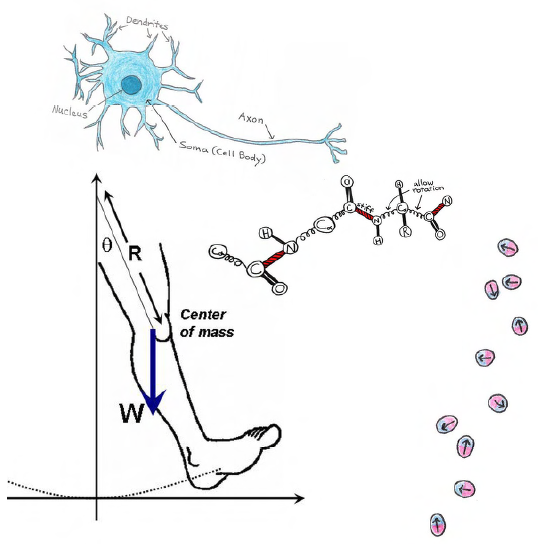
\includegraphics[width=\textwidth]{./figures/cover.png}
\end{titlepage}
\tableofcontents

\setcounter{chapter}{1}
\setcounter{section}{0}
\setcounter{figure}{0}
\setcounter{equation}{0}
\setcounter{table}{0}
\chapter*{
\includegraphics[width=\textwidth]{./figures/Topic1/Topic1.jpg}}
\addcontentsline{toc}{chapter}{Topic 1: Animal Locomotion}

\section{Introduction}

Imagine a giraffe, a Chihuahua, and an ant walking side by side without undue urgency. For every stride that the giraffe makes, the Chihuahua takes many and the ant many more. Most people intuitively know that the shorter the length of one’s legs, the faster they tend to swing. In other words, an inverse relation exists between the size of a creature and how quickly it can move its legs. Why would such a scaling relation exist?  
When walking at a leisurely pace, one may assume that the locomotion is executed in a way that minimizes energy expenditure.  A way to accomplish this is to let gravity do as much of the work whenever possible.  When an animal takes a step, the leg swings naturally from the hip, much like a pendulum in a gravitational field.  If the animal swings them faster or slower than their natural swinging time, you might think this may require undesirable additional energy expenditure. Thus, animals may want to swing their legs at precisely the natural swinging frequency of a pendulum in order to minimize energy expenditure. If so, does this account for why animals with shorter legs tend to swing them at a faster rate?  Let us set up the model and find out.

\section{Pendulum Motion}

\subsection{The Simple Pendulum: A Case in Point}

While almost any object can act as a pendulum, those that possess complex physical forms are difficult to analyze.  For this reason, we will begin by examining the most straightforward case: the simple pendulum in a gravitational field.  The simple pendulum is aptly named, for it simply consists of a point mass suspended from a massless string.  The string is made massless to avoid having to calculate its rotational inertia, which, as you may recall, is a quantity that depends on the distribution of mass.  If we think of the leg as a simple pendulum, it is as if the entire mass of the leg is concentrated in the foot.  Figure \ref{Fig1-1} below shows a simple pendulum of length $\ell$ and mass $m$.  As the pendulum oscillates, the point mass traces an arc of the circle of radius $\ell$.
\begin{figure}[htb]
\centering
	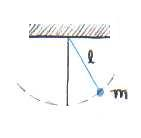
\includegraphics[width=2.5in]{./figures/Topic1/Figure1-1.jpg}
	\caption{The simple pendulum with length $\ell$ and mass $m$.}
	\label{Fig1-1}
\end{figure}

 
We are now ready to derive an equation that describes the position of the pendulum as a function of time.  From the equation, we will then obtain another equation that computes the stepping time for an animal.  
What are the forces acting on the mass?  The best way to visualize them is by drawing a force diagram (Figure~\ref{Fig1-2}).  
\begin{figure}[htb]
	\centering
	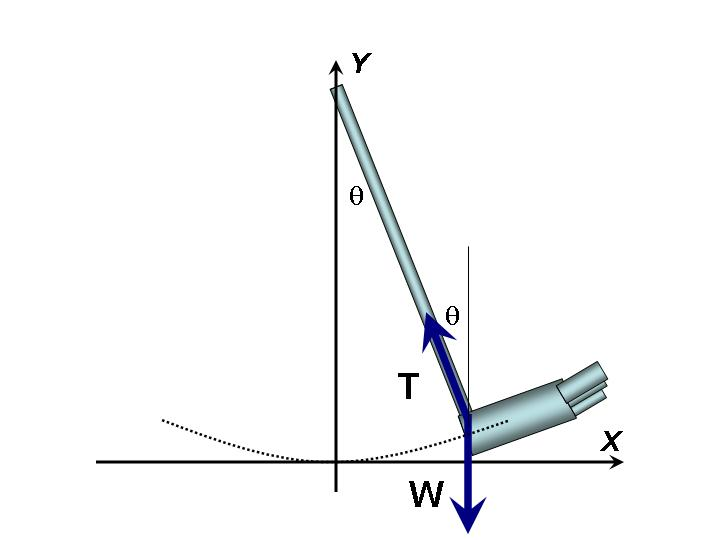
\includegraphics[width=3.0in]{./figures/Topic1/Figure1-2.jpg}
	\caption{Free-body diagram for mass m.}
	\label{Fig1-2}
\end{figure}

According to Newton’s 2nd Law, the sum of the forces along the $x$-axis and $y$-axis are equal to the mass, $m$, multiplied by the acceleration in the $x$-direction, $a_x$, and in the $y$-direction, $a_y$, respectively.
$$\sum F_x = ma_x$$
$$\sum F_y = ma_y$$
To simplify the problem, we will assume that the movement of the foot along the $y$-direction is always negligible compared to the one along the $x$-direction. This is approximately true when taking moderate steps, for which the angle $\theta$ rarely exceeds 20$^{\circ}$. If so, we may also ignore the acceleration of the foot along the $y$ when we invoke Newton’s second law. When taking this into account, and breaking down the forces into $x$ and $y$ components as shown in Fig.~\ref{Fig1-3}, we obtain 
\begin{figure}[htb]
	\centering
	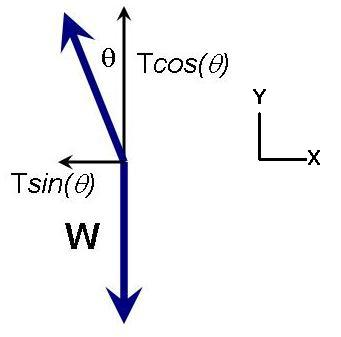
\includegraphics[width=2.5in]{./figures/Topic1/Figure1-3.jpg}
	\caption{Force diagram, with the tension, $T$, broken down into its $x$ and $y$ components.}
	\label{Fig1-3}
\end{figure} 

\begin{equation}\label{eqn1-1}
\sum F_x = T \sin\left(\theta\right) = ma_x
\end{equation}
\begin{equation}\label{eqn1-2}
\sum F_y = -w + T \cos\left(\theta\right) = 0
\end{equation}
When Eq.~\ref{eqn1-2} is solved for the tension ($T = w/ \cos(\theta)$), and this expression is substituted for $T$ in Eq.~\ref{eqn1-1}, we derive the following relation between $a_x$ and the weight 
\begin{eqnarray}\label{eqn1-3}
ma_x = -\frac{w}{\cos\left(\theta\right)} \sin\left(\theta\right) = -w \tan\left(\theta\right)
\end{eqnarray}

Since $w=mg$, we can simplify:
$$ma_x = -mg \tan\left(\theta\right)$$       
\begin{eqnarray}\label{eqn1-4}
a_x = -g \tan\left(\theta\right)             
\end{eqnarray}
Note that the acceleration is not constant, that is, it varies with the angle $\theta$, which is dependent on the position $x$ of the foot along the horizontal. Hence we cannot use simple approaches like the kinematic equations to solve for the time it takes to complete a step.  We will approach the solution to Eq.~\ref{eqn1-4} differently than what is done in an introductory physics course. 
Recall that the tangent of an angle can be defined as the ratio of the opposite and adjacent sides of a right triangle.
$$\tan\left(\theta\right)  = \frac{{\rm opposite}}{{\rm adjacent}}$$
In our case, as shown below in Fig.~\ref{Fig1-4}, the adjacent of angle $\theta$ is simply the length of the leg $\ell$. 
\begin{figure}[htb]
	\centering
	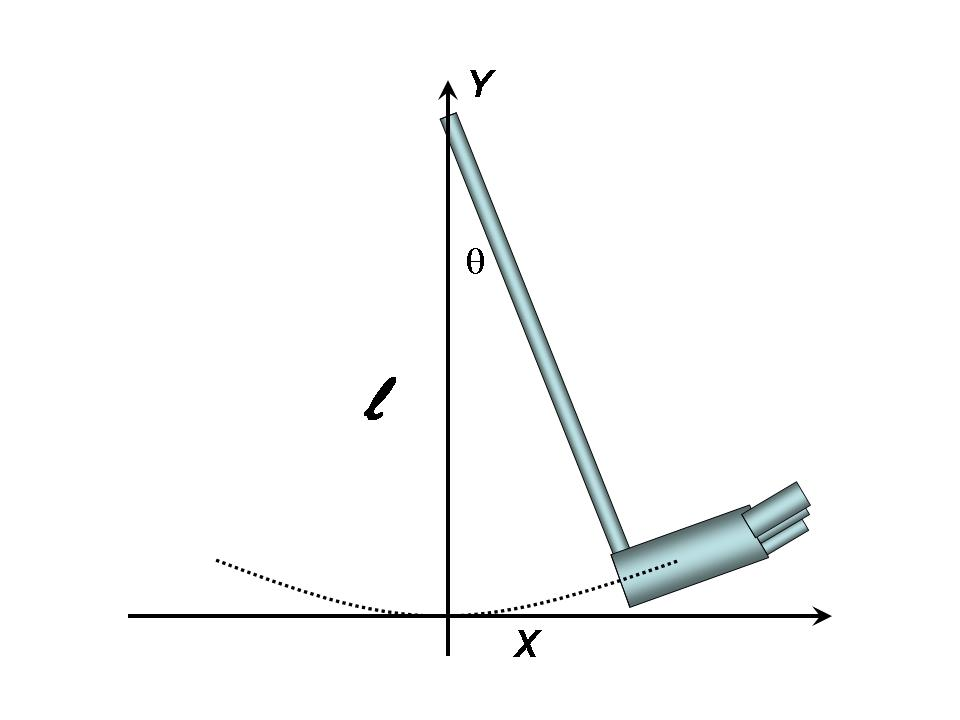
\includegraphics[width=2.5in]{./figures/Topic1/Figure1-4.jpg}
	\caption{Adjacent and opposite sides of the triangle defined by $\theta$.}
	\label{Fig1-4}
\end{figure} 
The opposite here corresponds to the displacement of the foot, or $x$, along the x-direction. Accordingly, $\tan\left(\theta\right) \approx x/l$, and Eq.~\ref{eqn1-4} becomes:
\begin{eqnarray}\label{eqn1-5}
a_x = -\frac{g}{\ell}x
\end{eqnarray}             
But ax also varies with position and time.  Recall that velocity is the first derivative of position with respect to time and that acceleration is the first derivative of velocity with respect to time.  It follows that acceleration is the second derivative of position with respect to time, written in differential form as:
\begin{eqnarray}\label{eqn1-6}
a_x = \frac{d^2x}{dt^2}
\end{eqnarray}      
Substituting Eq.~\ref{eqn1-4} into Eq.~\ref{eqn1-5}, we arrive at the equation we must solve for $x$:
\begin{eqnarray}\label{eqn1-7}
\frac{d^2x}{dt^2} = -\frac{g}{\ell}x
\end{eqnarray} 
Eq.~\ref{eqn1-7} is of a type known as a ``differential equation'' because it contains a derivative of what you solving for. Since solving differential equations is beyond the scope of the course, the steps are left to the more ambitious student.  However, as you will verify in one of your homework problems, the following solutions satisfy Eq.~\ref{eqn1-7}.
\begin{eqnarray}\label{eqn1-8}
x = A \sin\left(\sqrt{\frac{g}{\ell}}~t\right)
\end{eqnarray}
or
\begin{eqnarray}\label{eqn1-9}
x = A \cos\left(\sqrt{\frac{g}{\ell}}~t\right),
\end{eqnarray}
where $A$ is a constant. \footnote[1]{The procedure is quite simple.  To verify for example that Eq.~\ref{eqn1-8} is a solution, first take the second derivative of the right hand side. Then show that with some algebraic manipulation that it equals $-(g/l)x$ as Eq.~\ref{eqn1-7} suggests.}

The constant, $A$, in each case refers to the amplitude of the step, and we can visualize the motion in terms of its oscillatory behavior, shown in Figure\ref{Fig1-5}.
\begin{figure}[htb]
	\centering
	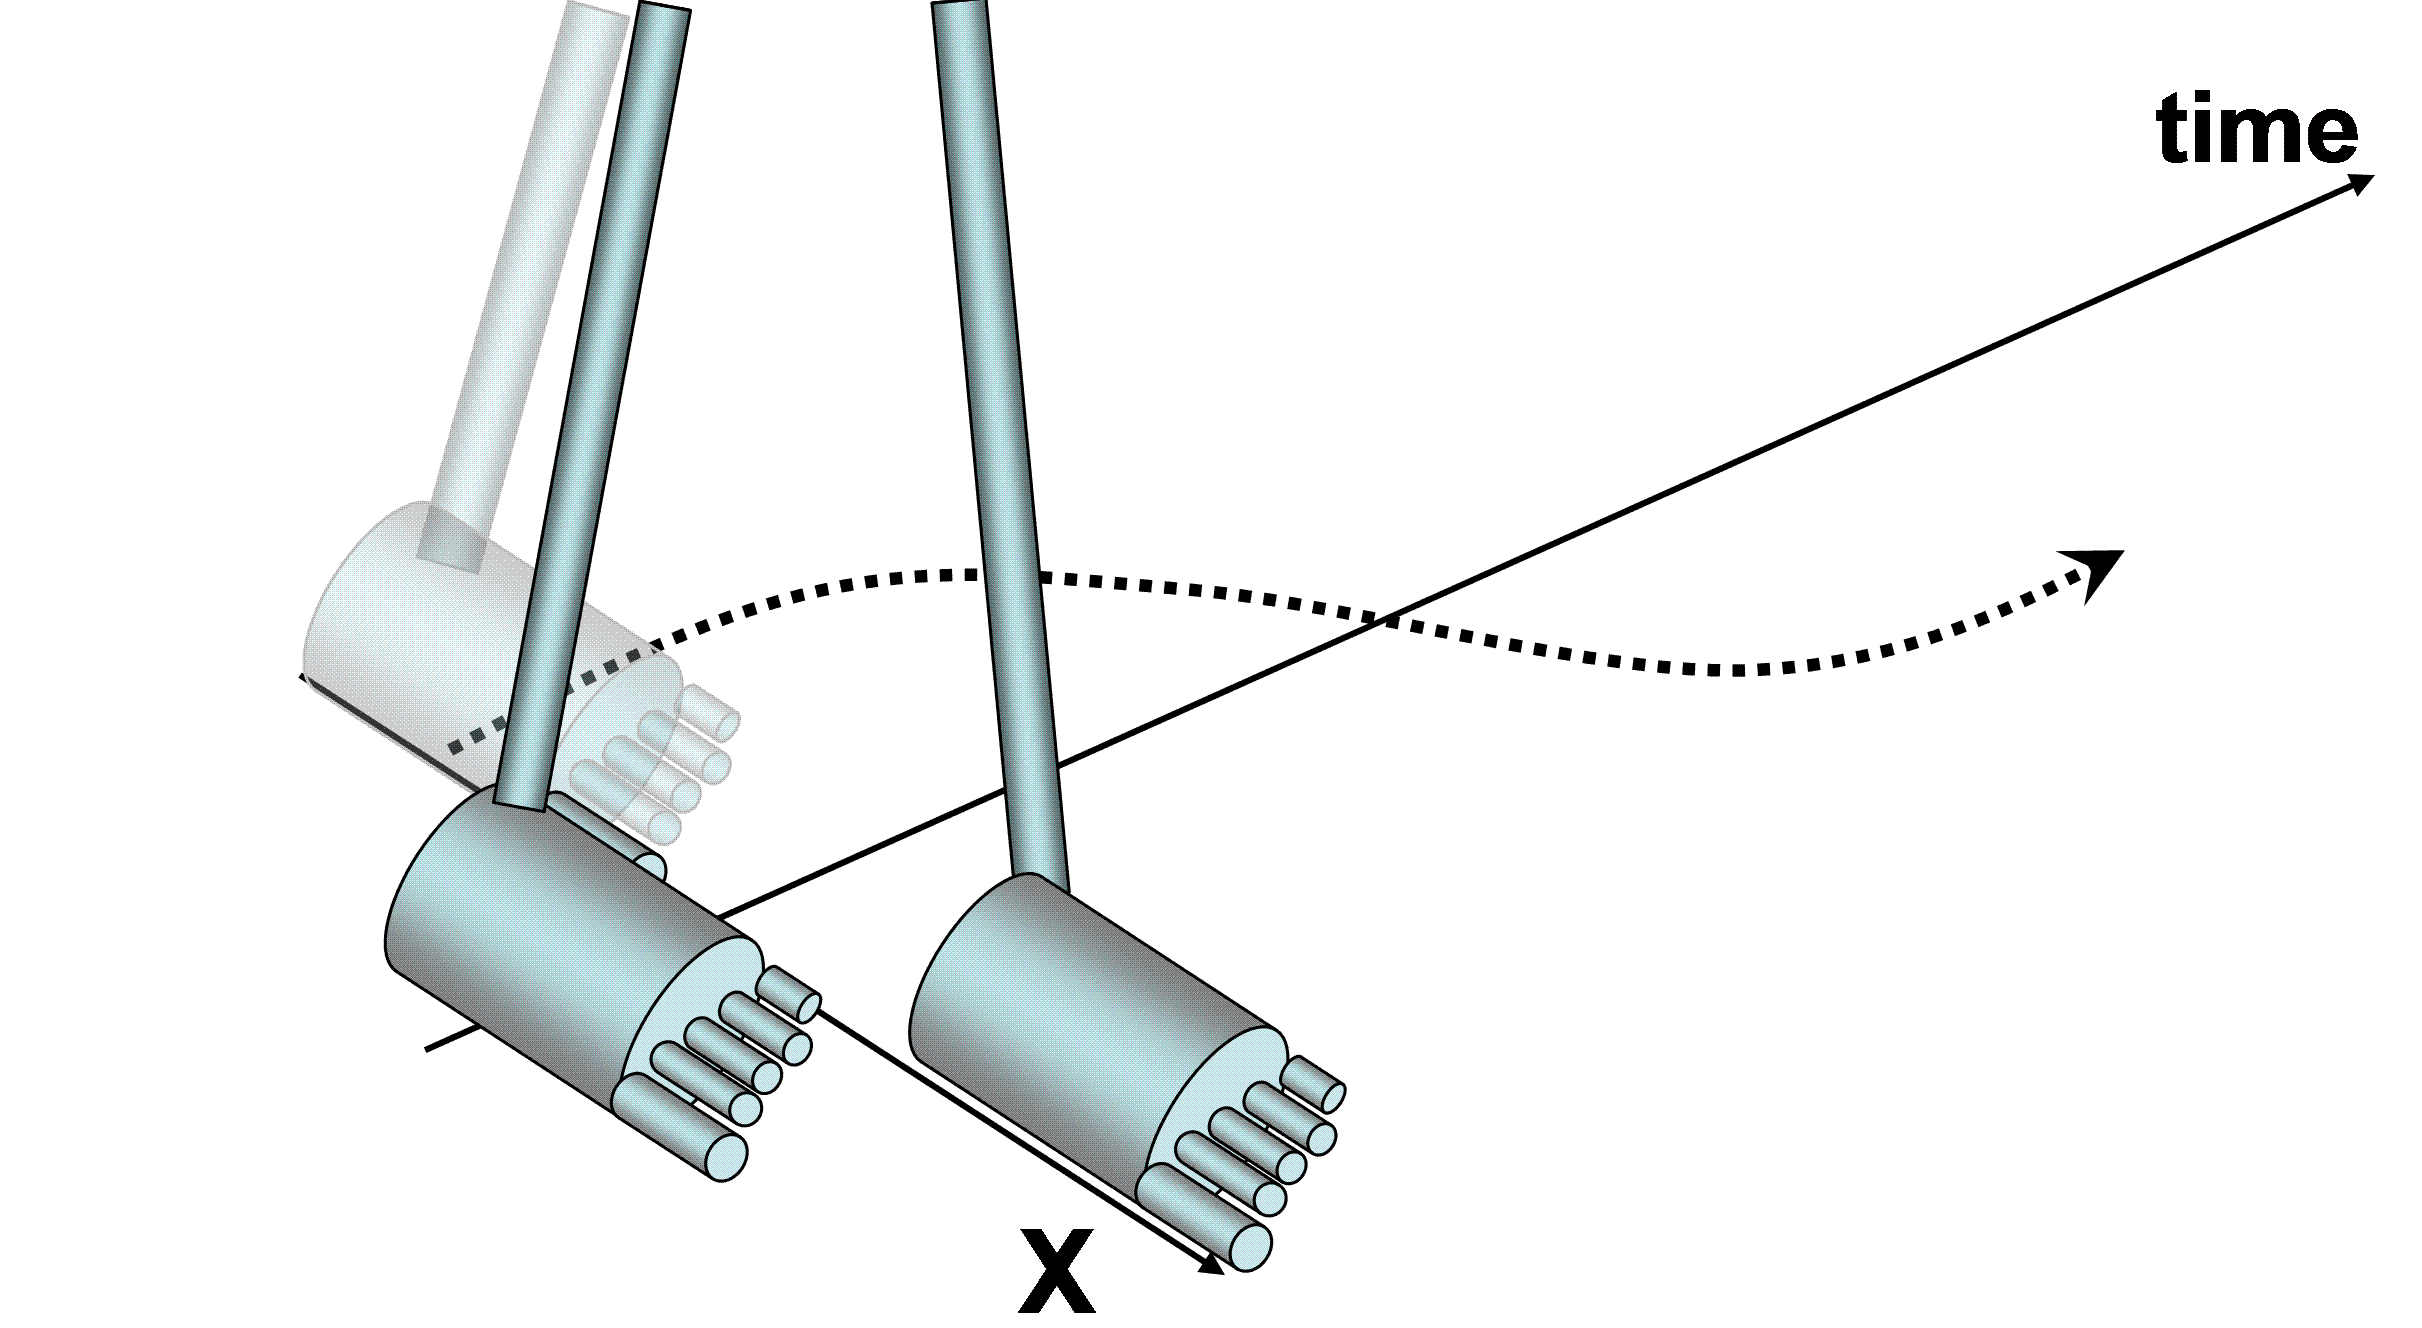
\includegraphics[width=2.25in]{./figures/Topic1/Figure1-5a.png}
	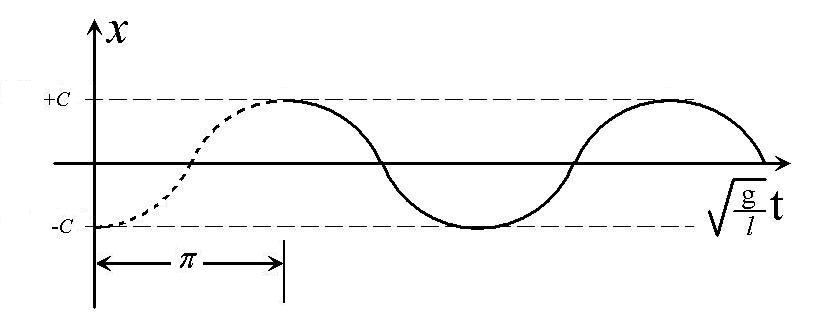
\includegraphics[width=3.25in]{./figures/Topic1/Figure1-5b.png}
	\caption{As the back leg moves forward it undergoes motion corresponding to half of a full pendulum oscillation.}
	\label{Fig1-5}
\end{figure}
From Fig.\ref{Fig1-5} we see that a step corresponds to one half of the full sinusoidal oscillation. In terms of our solutions Eq~\ref{eqn1-8} and Eq.~\ref{eqn1-9}, this corresponds to a time such that 
\begin{eqnarray}\label{eqn1-10}
\pi = \sqrt{\frac{g}{\ell}}\tau
\end{eqnarray}
Solving for $\tau$, we get the theoretical time it takes for the leg to step forward:
\begin{eqnarray}\label{eqn1-11}
\tau = \pi\sqrt{\frac{\ell}{g}}
\end{eqnarray}
Interestingly enough, in this model, the mass of the body or leg does not affect how long it takes for an animal to take a step; only the leg length and the magnitude of gravity are determining factors.  Note that the stepping time $\tau$ varies with the square root of $\ell$, proving that our intuition is correct—longer legs do require more time to take a step.

How accurately does Eq.~\ref{eqn1-11} predict stepping time?  The leg of the average adult human is approximately 0.9 m, corresponding to a theoretical stepping time of 0.95 s.  Biophysics students measure $\tau$ as part of a laboratory activity, finding it to be closer to 0.6-0.7 s.  The error is about 50\%, which is relatively small when one considers that the human leg looks nothing like a point mass attached to a massless string.  In the next section, we will improve the model by taking into account the distribution of mass in the leg.  

\subsection{The Physical Pendulum: A Refined Model}

Contrasted with the simple pendulum where the mass is concentrated at a point, the physical pendulum approach is capable of handling any arbitrary distribution of mass that swings about a fixed pivot.  Examine the diagram shown below for a human leg swinging as a physical pendulum.
\begin{figure}[htb]
	\centering
	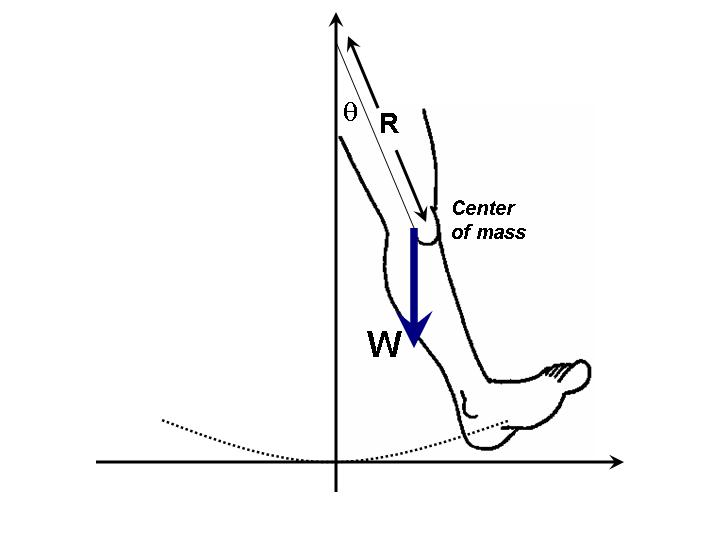
\includegraphics[width=3.5in]{./figures/Topic1/Figure1-6.jpg}
	\caption{Free body diagram of the physical pendulum.}
	\label{Fig1-6}
\end{figure}
  
A significant difference between the simple pendulum and the physical pendulum models is that the first looks at the action of forces, whereas the second focuses on torques. Recall that a torque is the turning force that causes objects to rotate about a pivot point. The strength of the torque is dependent not only on the applied force but also on distance from where it is applied to the pivot point. In this case, gravity is the only force that causes rotational motion, and the magnitude of the torque associated with this force is the force $F$ times the distance from where it is applied to the pivot point ($R$). In addition, the product must be multiplied by the sine of the angle between the directions of the force and the line of action which connects the pivot point to the center of mass. The resulting expression is $w R \sin\theta$, or $m g R \sin\theta$, where $R$ is the distance from the pivot point to the center of mass.  Note that in Fig.~\ref{Fig1-6} the direction of the torque (clockwise) opposes the angular displacement $\theta$ (counter-clokwise). This is always the case, even if the leg is to the left of the centerline; in that case the direction of the angular displacement is clockwise whereas that of the torque is counter-clockwise. 
The sum of the torques acting on the mass obeys the equation
\begin{eqnarray}\label{eqn1-12}
\sum \tau = I\alpha
\end{eqnarray}
where $\tau$ is now defining torque rather than a characteristice time, $I$ is the moment of inertia and $\alpha$ is the angular acceleration.  Recall that the moment of inertia takes into account the distribution of mass of the leg.  In fact, if you divide the leg into small masses, and identify each mass $m$ with an index $n$, the moment of inertia is given by the formula  $$I=\sum_n m_n R_n^2.$$  
Angular acceleration, $\alpha$ is the second derivative of $\theta$ with respect to time.  Thus, Eq.~\ref{eqn1-12} can be rewritten as
\begin{eqnarray}\label{eqn1-13}
-R m g \sin\left(\theta\right)=I\frac{d^2\theta}{dt^2}
\end{eqnarray}
Rearranging, we get:
\begin{eqnarray}\label{eqn1-14}
\frac{d^2\theta}{dt^2} = -\frac{Rmg}{I}\sin\theta
\end{eqnarray}
As we stated earlier, an animal’s leg rarely subtends an angle greater than 20$^{\circ}$ relative to the normal while walking.  This means that that we can take advantage of the small angle approximation, which states that for angles less than 20$^{\circ}$, $\sin\theta \approx \theta$.  (Recall that the small angle approximation only holds when the angle is expressed in radians.)  Eq.~\ref{eqn1-14} simplifies to
\begin{eqnarray}\label{eqn1-15}
\frac{d^2\theta}{dt^2} = -\frac{RMg}{I}\theta
\end{eqnarray}
Compare Eq.~\ref{eqn1-7} to Eq.~\ref{eqn1-15}.  Instead of $x$, we now have $\theta$, and instead of the constant $g/\ell$, we now have $Rmg/I$.  Observing these substitutions makes solving Eq.~\ref{eqn1-15} easy, because we have already solved Eq.~\ref{eqn1-7}. The solutions are of the form: 
\begin{eqnarray}\label{eqn1-16}
\theta(t) = A \sin\left(\sqrt{\frac{Rmg}{I}}t\right)
\end{eqnarray}
or
\begin{eqnarray}\label{eqn1-17}
\theta(t) = A \cos\left(\sqrt{\frac{Rmg}{I}}t\right)
\end{eqnarray}
Also analogous to the previous case, a step corresponds to the time when the period is 
\begin{eqnarray}\label{eqn1-18}
\pi = \sqrt{\frac{Rmg}{I}}t
\end{eqnarray}
and the stepping time is
\begin{eqnarray}\label{eqn1-19}
\tau = \pi\sqrt{\frac{I}{Rmg}}
\end{eqnarray}
As stated above, the moment of inertia $I$ of an object pivoting about an axis is found by first breaking down the object into small pieces each with the same mass $m$. After identifying each mass $m$ with an index $n$, the moment of inertia is given by the formula $I=\sum_n m_nR_n^2$.   Most physics textbooks list the result of this calculation for the moments of inertia of various bodies with simple geometries. To take advantage of these existing formulas for $I$, we can assume a simplified shape for the leg by thinking of it as a slender rod with a pivot through one end (the hip).  Accordingly, 
$$I=\frac{1}{3}m\ell^2$$
$$R = \frac{1}{2}\ell$$
where $\ell$ is the length of the leg and $m$ is the total mass of the leg. If we substitute these equations into Eq.~\ref{eqn1-19}, we get an equation that calculates the stepping time, accounting for the continuous mass distribution of the leg.
\begin{eqnarray}\label{eqn1-20}
\tau = \pi\sqrt{\frac{2\ell}{3g}}
\end{eqnarray}
This equation is almost identical to Eq.~\ref{eqn1-11} for the simple pendulum case, with the exception of a new constant, $\sqrt{2/3}$, which is approximately 0.8.  The new factor makes the theoretical stepping time $\tau$ = 0.78 s, which is about 20\% lower than when computed using the simple pendulum model.  Now the theoretical time more closely matches the experimental measurements for adult humans, which was in the range of 0.6 to 0.7 s.

One might be tempted to think that leg length is the only variable that affects the stepping time.  However, $\tau$ is just as dependent on the gravitational constant.  Eq.~\ref{eqn1-20} explains why astronauts move differently on the moon, where $g$ is about 1/6 of Earth’s value.  Because of the diminished $g$, each step takes about 2.5 (or $\sqrt{6}$) times as long as on Earth. The increased stepping time apparently became unbearably long for these astronauts, who immediately found that to get from point A to point B quickly, it was more efficient to hop than to walk.  This incident also underscores how our bodies have adapted to the gravitational environment in which we live. %Locomotion
\setcounter{chapter}{2}
\setcounter{section}{0}
\setcounter{figure}{0}
\setcounter{equation}{0}
\setcounter{table}{0}
\chapter*{
\includegraphics[width=\textwidth]{./figures/Topic2/Topic2.jpg}}
\addcontentsline{toc}{chapter}{Topic 2: Fluid Mechanics of the Circulatory System}

\section{Introduction}

Single-cell organisms live in direct contact with the environment from where they derive nutrients and into where they dispose of their waste. For living systems containing multiple cells, there is the challenge of how to get nutrients past multiple layers of cells efficiently and how to avoid the build-up in waste products within deep cellular layers. The answer to these challenges is the development of an intricate plumbing network, containing pumps and distribution lines that are collectively called the circulatory system.  

\begin{wrapfigure}{r}{0.5\textwidth} 
\vspace{-20pt}
  \begin{center}
    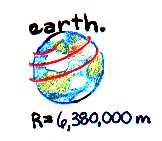
\includegraphics[width=0.4\textwidth]{./figures/Topic2/Earthclip.jpg}
    %\caption{}
%    \label{fig:databaseUserTable}
  \end{center}
  \vspace{-20pt}
  \vspace{1pt}
\end{wrapfigure} 
To give you a sense for the complexity of the human circulatory system consider the following facts. Lined up end-to-end, your blood vessels would wrap more than twice around the Earth, and your circulatory system pumps over five liters of blood through the body every minute.  Meandering through vast networks of capillaries, blood delivers oxygen and nutrients to the body’s cells at a leisurely 0.026cm/s.  In contrast, it rushes through the aorta at 30cm/s, over a thousand times faster.
 
The pressure in the circulatory system also undergoes changes as it traverses blood vessels of differing diameters and as it defies or succumbs to gravity.  Thus as we shall see, pressure is usually higher in the arteries than in the veins, but it also varies with posture. This is why accident victims are directed to keep bleeding wounds raised above heart level; this action lowers the blood pressure in the wound, and consequently lessens the bleeding.  
Applying the laws of fluid mechanics to blood flow not only helps us understand the factors governing circulation, but lets us design better medical instruments and more effective treatments for diseases and accidents involving the circulation.  

\section{Fluid Dynamics of Human Circulation}

\subsection{Pressure and flow rate along a pipe: a few fundamental concepts} 

A fluid can move one way inside a pipe only if the fluid is pushed with a greater force from one side than from the other, i.e. if a pressure difference exists between the ends of the pipe. For example, when one end of a hose is connected to a faucet and the other placed over a drain, the water inside the hose experiences a pressure difference. That is, the side connected to the faucet is subjected to a high pressure (typically 60 PSI) whereas the side that empties into the drain is at 0 PSI. The pressure inside the hose varies accordingly from 60 PSI for a point near the faucet to 0 PSI at another point near the drain. In between, the pressure varies gradually between those two extremes (see Fig.~\ref{Fig2-1}).
\begin{figure}[htb]
	\centering
	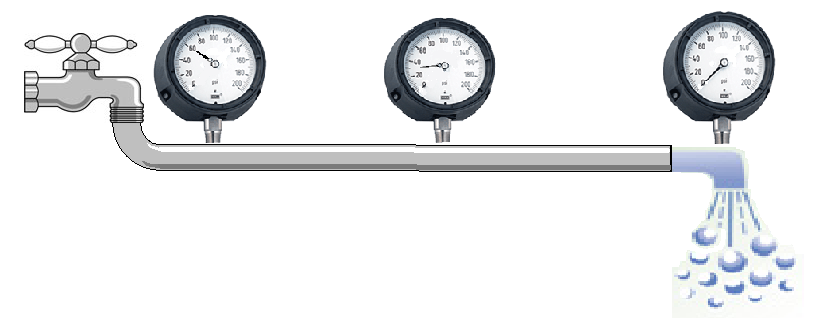
\includegraphics[width=\textwidth]{./figures/Topic2/Fig2-1.png}
	\caption{Pressure drops gradually but flow rate remains the same throughout the pipe.}
	\label{Fig2-1}
\end{figure}

The fluid flow rate, i.e. the volume of fluid flowing through the hose per unit time (e.g. gallons,/min or cc/min), is directly proportional to the pressure difference across the ends. Unlike pressure, which drops gradually along the length of the hose, the flow rate at any point is always the same. That is, what goes into the hose in a given amount of time must come out over the same time. This is simply a reflection of conservation of mass. Were this not the case, mass would accumulate or vanish within the pipe. 

The system depicted in Fig.\ref{Fig2-1} is an example of an open system, i.e. one where the fluid is lost at the drain side. Obviously this is not a desirable design for a circulatory system where blood must be preserved. A closed system, i.e. one where blood is recycled back into the starting point, is thus absolutely necessary for the function of an animal. To accomplish this, a pump must exist to recycle the fluid back and to pressurize it once more so that its flow is maintained constant throughout the system. The heart fulfills that function. 

\subsection{The Systemic and Pulmonary Systems}

In addition to the need for a pump, the circulatory system requires constant intaking of oxygen and expelling of carbon dioxide that accumulates from metabolic processes. This gas exchange function is performed by the lungs, an organ that must therefore be an integral part of the circulatory system as important as the heart. 

The need to enrich blood with oxygen before delivering it to the body poses an interesting hydrodynamic challenge for the circulatory system that is illustrated in Fig.~\ref{Fig2-2}(a). Fish employ such a simple design. As blood traverses the network of capillaries within the gills it loses much pressure, but enough remains to push blood at rates that meet the fish’s demand for oxygen. Mammals, however, have much higher metabolic rates and thus must consume more oxygen. The pressure out of the lungs would be insufficient to push blood at rates needed to deliver sufficient oxygen for the rest of the body. To circumvent this problem, animals have evolved a circulatory system that includes the dual pumping system illustrated in Fig.~\ref{Fig2-2}(b). The second pump increases the pressure to a level sufficient to push blood throughout the body. 
\begin{figure}[htb]
	\centering
	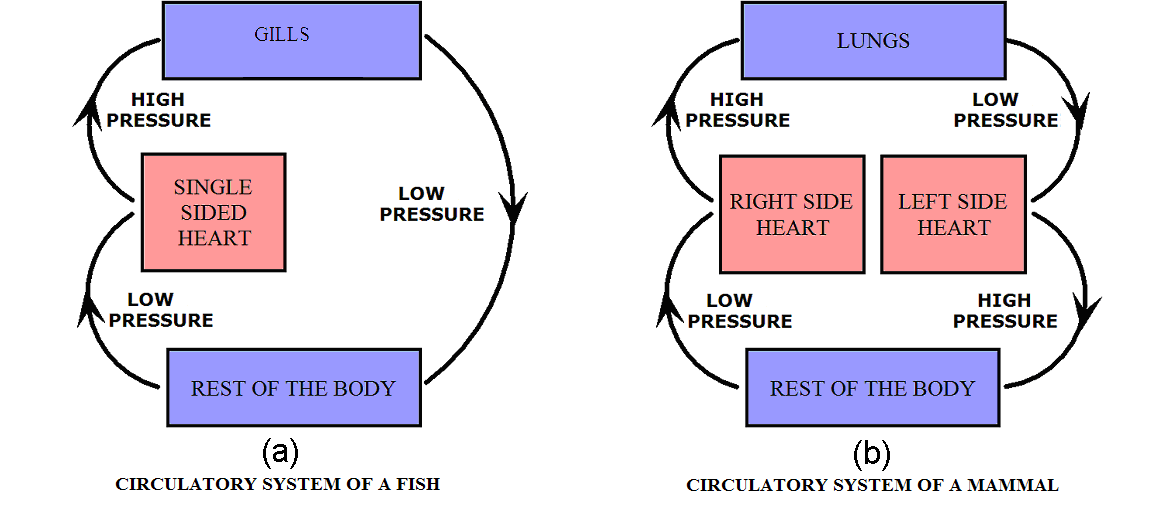
\includegraphics[width=\textwidth]{./figures/Topic2/Fig2-2.png}
	\caption{Diagram of flow through air intake and the rest of the body. High and low pressure areas are indicated.}
	\label{Fig2-2}
\end{figure}

The mammalian heart has four chambers, allowing it to serve as a pump for two distinct circuits: the pulmonary system, which pumps blood through the lungs, and the systemic system, which services the rest of the body.  Two of the chambers, called atria, collect blood entering the heart and pump it to the other two chambers, called ventricles, which pump it throughout the body.  (See Figure \ref{Fig2-3}.)  In the pulmonary circuit, blood leaves the right ventricle via the pulmonary arteries and passes through capillary beds in the lungs, where carbon dioxide is exchanged for oxygen.  The oxygen-rich blood then returns to the heart, moving through the pulmonary veins to the left atrium.  Next it flows to the left ventricle, where it is forcefully pumped through the aorta to the rest of the body.  Two large veins called vena cavae (superior and inferior) collect the oxygen-poor blood and return it to the heart, depositing it in the right atrium.  
\begin{figure}[htb]
	\centering
	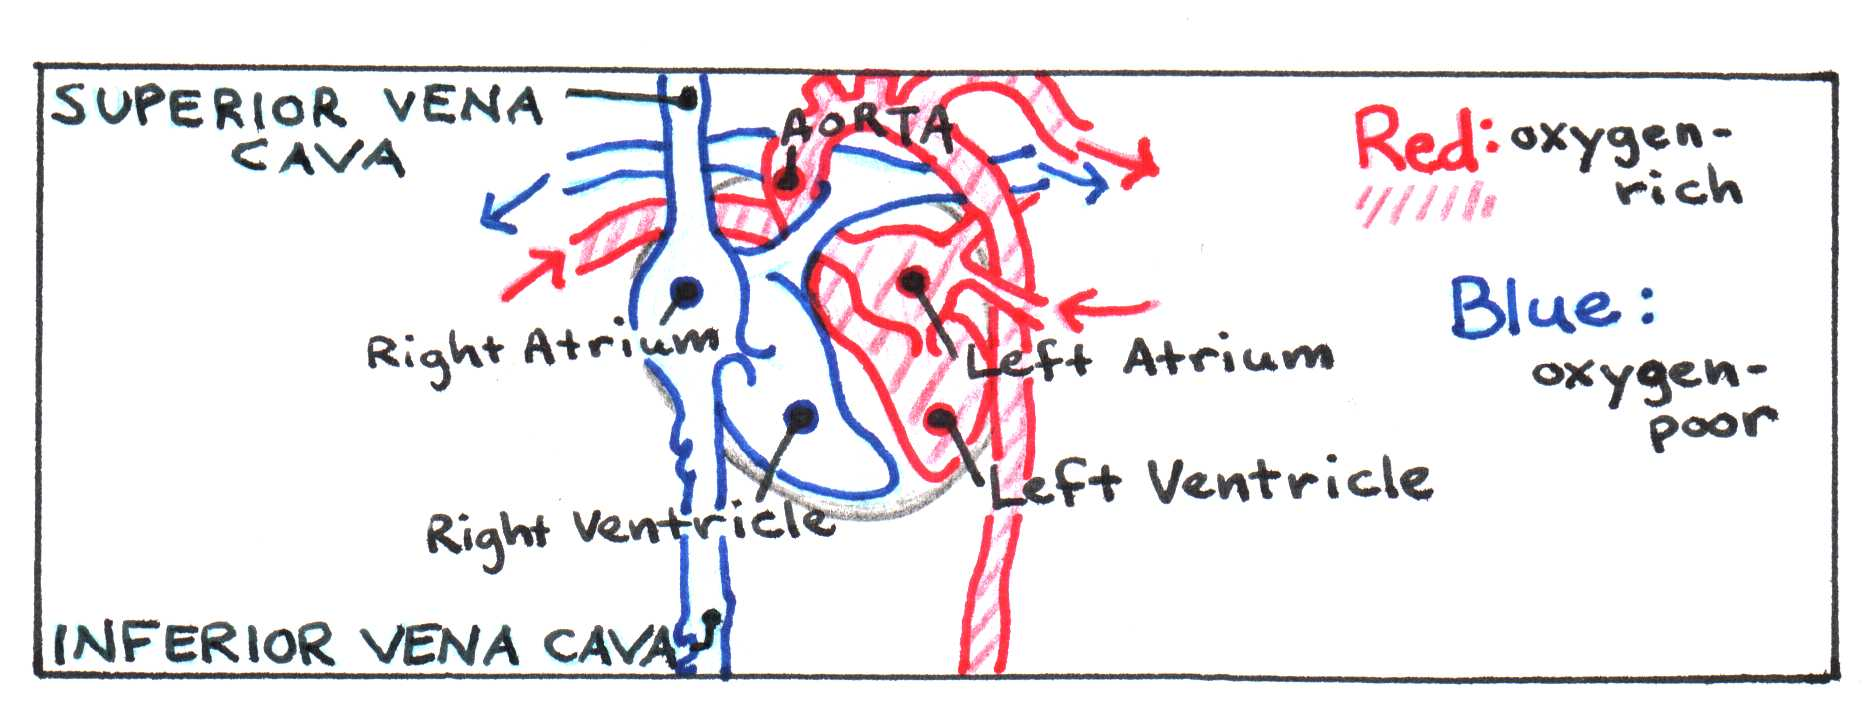
\includegraphics[width=\textwidth]{./figures/Topic2/Fig2-3.jpg}
	\caption{Diagram of flow through the heart.}
	\label{Fig2-3}
\end{figure}  

In either system, arteries carry blood away from the heart, branching into smaller blood vessels called arterioles.  These branch further into microscopic capillaries that network through tissues, allowing chemical exchange to occur.  Downstream of capillary beds, the capillaries converge into venules, which in turn converge into veins.  Veins bring blood back to the heart, completing the circuit.

In both the systemic and pulmonary systems, valves in the heart allow pressure to build before the blood is pumped out of the heart.  Blood travels further in the systemic system than in the pulmonary system, so pressure in the aorta must be much greater than in the pulmonary arteries.  Figure \ref{Fig2-4} illustrates the pressure differences in the different parts of the circulatory system.
\begin{figure}[htb]
	\centering
	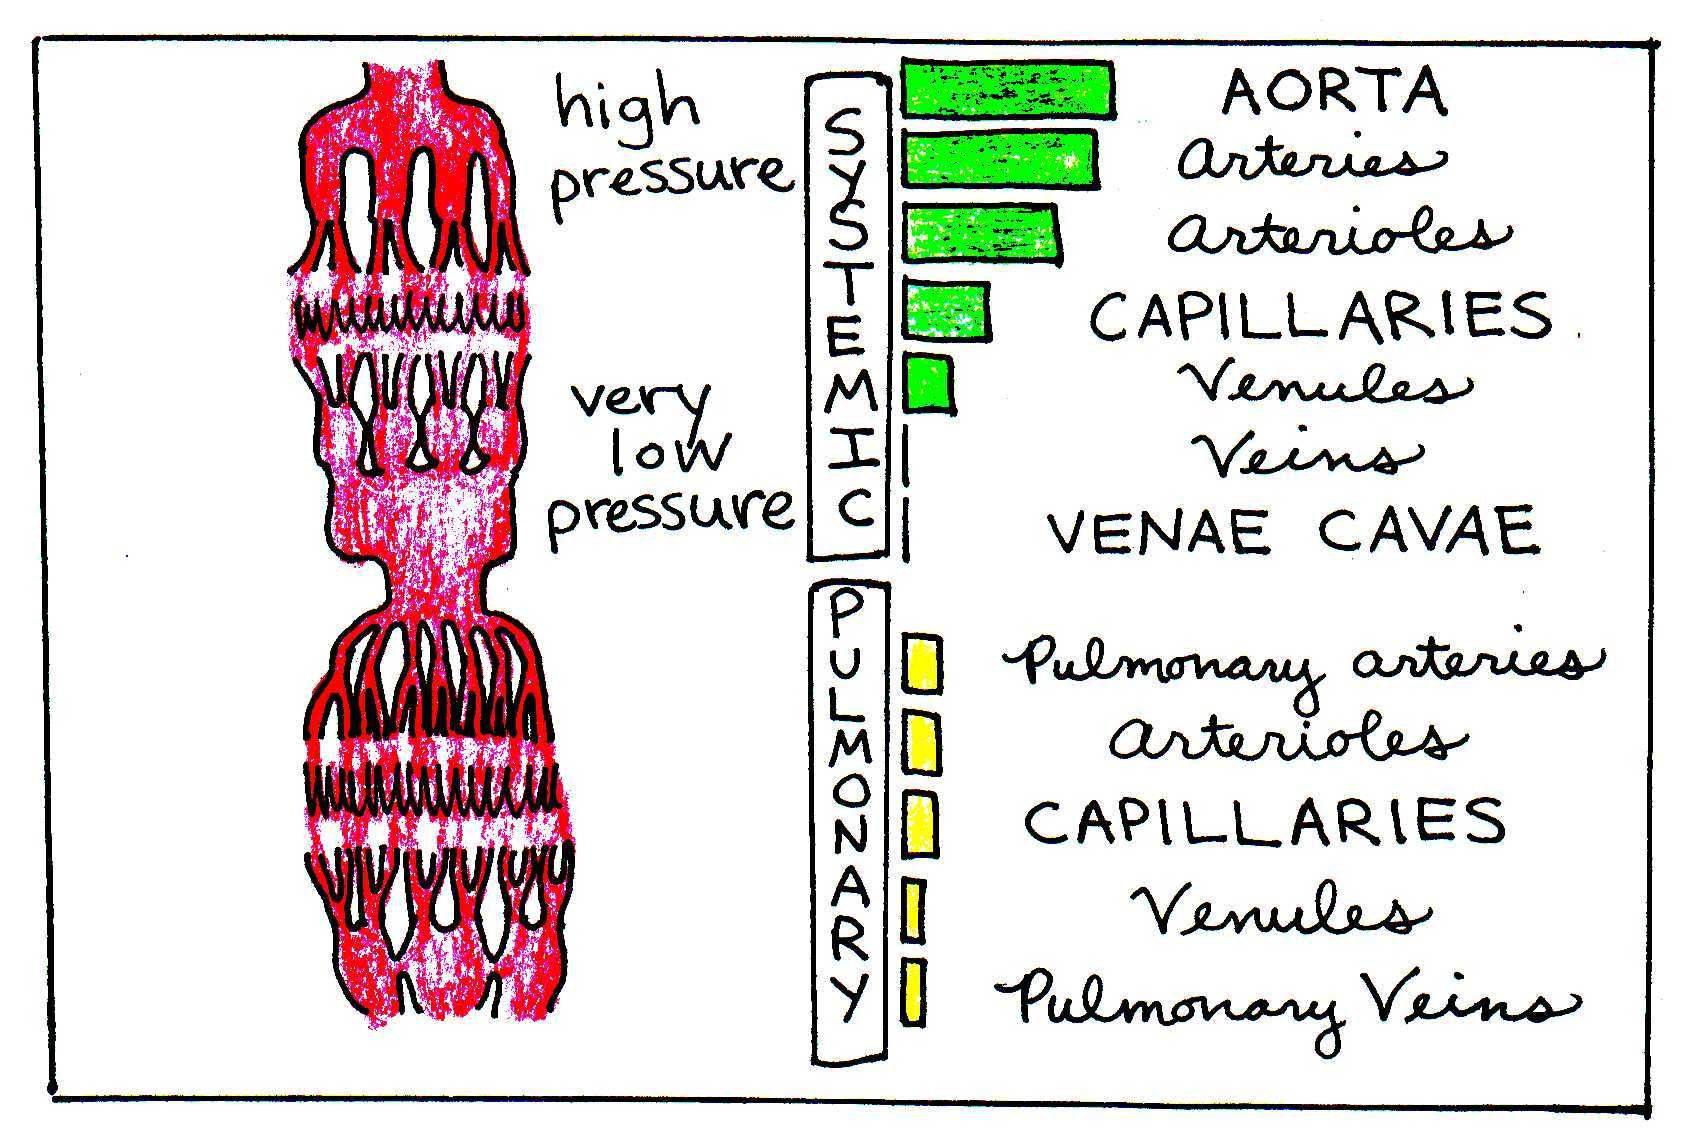
\includegraphics[width=\textwidth]{./figures/Topic2/Fig2-4.jpg}
	\caption{The green and yellow bars illustrate the varying levels of blood pressure in the different portions of the circulatory system.}
	\label{Fig2-4}
\end{figure}

\subsection{The Continuity Equation}

The volume flow rate through a pipe is defined as the volume of the fluid that passes a particular point per unit time.  We can quantify it by multiplying the cross-sectional area $A$ of the pipe by the velocity of the fluid $v$, which is distance covered per unit time. This is diagrammed in Fig.~\ref{Fig2-5}.
\begin{figure}[htb]
	\centering
	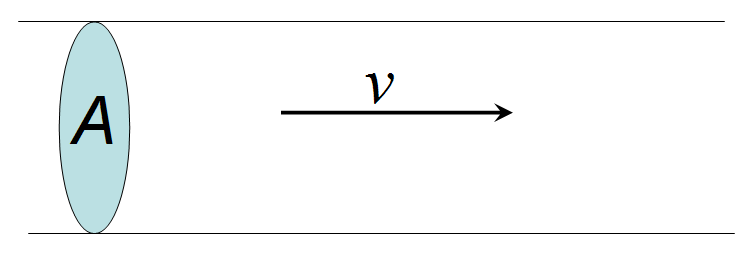
\includegraphics[width=3.5in]{./figures/Topic2/Fig2-5.png}
	\caption{Schematic of fluid flow at velocity, $v$ passing through a cross-sectional area, $A$.}
	\label{Fig2-5}
\end{figure}
\begin{equation}\label{eqn2-1}
\frac{dV}{dt} = Av
\end{equation}

Note that this gives the correct units of the flow rate: cm$^3$/s. Since blood is not compressible, volume is preserved unless there is a break in a blood vessel.  It follows, then, that the volume flow rate remains constant everywhere, since the flow is circular.  This means that a fluid moving through a wide vessel must move more quickly when the vessel narrows.  This relationship between cross-sectional area and velocity in different portions of the circulatory system is expressed by the continuity equation:
\begin{equation}\label{eqn2-2}
\frac{dV}{dt} = A_{aorta}v_{aorta} = A_{capillary}v_{capillary}
\end{equation}
where $A_{aorta}$ is the cross-section of the aorta and $A_{capillary}$ is the combined cross-section of all the capillaries. If we could lump all the blood vessels together by class, the circulatory system could be visualized as a pipe circuit, as in Figure \ref{Fig2-6}.
\begin{figure}[htb]
	\centering
	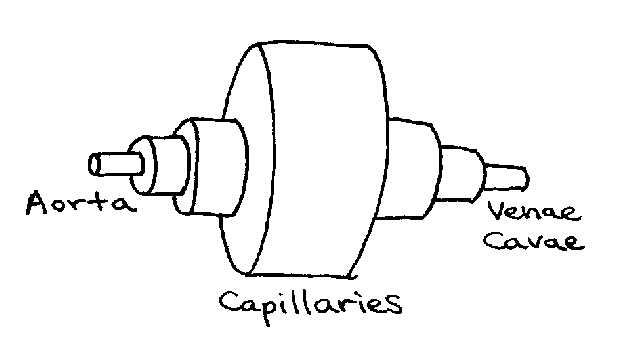
\includegraphics[width=4in]{./figures/Topic2/Fig2-6.jpg}
	\caption{Pipe circuit analogous to circulatory system. Note that each section represents the effective diameter of a particular type of vessel (e.g. capillaries) after all vessels of that type are combined.}
	\label{Fig2-6}
\end{figure}
Table \ref{table2-1} below gives the total cross-sectional area of the blood vessels within each part of the system.
\begin{table}[htb]
\begin{center}
\begin{tabular}{|l|c|}
\hline
Vessel & Area (cm$^2$) \\
\hline
aorta & 2.5 \\
small arteries & 20 \\
arterioles & 40 \\
capillaries & 2600 \\
venules & 250 \\
small veins & 80 \\
venae cavae & 8 \\
\hline
\end{tabular}
\caption{Total cross-sectional area of all blood vessels in humans.}
\label{table2-1}
\end{center}
\end{table}
The volume flow rate out of the heart into the aorta is roughly 80 ml/s.  By using this value and A = 2.5 cm$^2$ from Table 1, we use Eq.~(1) to calculate the corresponding velocity of blood in the aorta to be 32 cm/s.  Similarly, we can find the velocity of blood through the capillaries:  $dV/dt = 80 cm^3/s = A_{capillary}v_{capillary}$.  Using A = 2600 cm$^2$ from Table \ref{table2-1}, we find that $v_{capillaries}$ = 0.031 cm/s, roughly a thousand times slower than in the aorta.

Because of the inverse relationship between area and velocity in the continuity equation, we might be tempted to think that blood flows much faster through the tiny capillaries than through the huge veins and arteries.  This logic is misleading, however the total cross-sectional area is what matters, not the area of an individual blood vessel.

\subsection{Hydrostatics}
 
Fluid flow is described in general by Bernoulli's equation.
\begin{equation}\label{eqn2-3}
P_1 + \rho g y_1 + \frac{1}{2}\rho v_1^2 = P_2 + \rho g y_2 + \frac{1}{2}\rho v_2^2
\end{equation}
where the variables $P$, $y$, and $v$ represent the pressure, elevation, and velocity, respectively, of a fluid at a given point as shown below in Fig.~\ref{Fig2-7}.
\begin{figure}[htb]
	\centering
	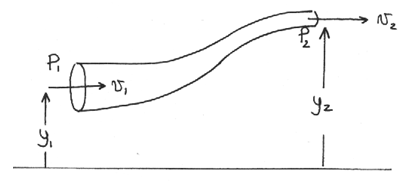
\includegraphics[width=\textwidth]{./figures/Topic2/Fig2-6.png}
	\caption{Diagram of a fluid flow tube with labels pertaining to Bernoulli's Equation.}
	\label{Fig2-7}
\end{figure}
When the velocity terms are negligible\footnote[2]{Proof is left as a homework assignment.}, as is often the case in the circulation, Eq.~\ref{eqn2-3} reduces to 
\begin{equation}\label{eqn2-4}
P_1 + \rho g y_1 = P_2 + \rho g y_2
\end{equation}
By combining the $\rho g y$ terms, the equation becomes even simpler.
\begin{equation}\label{eqn2-5}
P = P_{\circ}+ \rho g h,
\end{equation}
$P_{\circ}$ is the pressure at an arbitrary reference point (in our case, the heart), and $h = y_2-y_1$ is the depth of the fluid below that point. This equation reflects the well-known phenomenon of increased pressure with depth.  The mean arterial pressure for a human lying down is 100 mmHg (1 mmHg = 133 Pa). However, in an upright human, that arterial pressure can vary from 90 mmHg in the brain to 190 mmHg in the feet. The corresponding venous pressure can vary from -10 to 90 mmHg. These pressure values are relative to atmospheric pressure (i.e. gauge pressure).

\subsection{Effects of Viscosity}

Viscosity refers to the internal friction of a fluid resulting when layers of the fluid rub past each other.  This happens all the time inside pipes where layers adjacent to the walls move slower than layers deep inside the pipe.  Like any other frictional phenomenon, viscosity causes the fluid to gradually slow down.
Imagine standing on a bridge over a creek, dropping leaves into the water.  The leaves that fall near the center of the stream float along much faster than the ones that land near the water’s edge.  In the same way, blood at the center of a blood vessel moves at a higher velocity than it does along the walls.  It helps to think of the blood as being partitioned in concentric cylindrical layers, each moving at a slightly different speed.  Figure \ref{Fig2-8} illustrates this concept.  
\begin{figure}[htb]
	\centering
	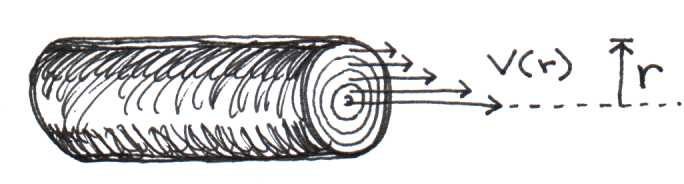
\includegraphics[width=4in]{./figures/Topic2/Fig2-7.jpg}
	\caption{Blood moves in concentric layers.  Layers closest to the center move fastest.}
	\label{Fig2-8}
\end{figure}
Viscosity arises because of the frictional force created between adjacent layers of the fluid that are moving at different speeds. The magnitude of the frictional force $F$ is directly dependent on the velocity difference $dv$ of the two layers separated by a distance $dr$, as well as the surface area of contact between them. The frictional force between two sheets is given by 
\begin{equation}\label{eqn2-6}
F = \eta A \frac{dv}{dr}
\end{equation}
where $\eta$ (greek letter ``eta'') is the viscosity and $A$ is the area of the common surface between layers.  In longer vessels, the effects of viscosity are more pronounced, because the common surface area between layers is increased. Calculations involving frictional forces are traditionally performed in the cgs (centimeters-grams-seconds) system of units, rather than in the SI system.  Thus, for example, the unit of force in the cgs system, called a dyne, is expressed in g$\cdot$cm/s$^2$ instead of kg$\cdot$m/s$^2$ for the Newton in the SI system. The unit of viscosity $\eta$ is called the poise, where 1 poise = 1 dyne$\cdot$s/cm$^2$. Table \ref{table2-2} is a set of conversions that you will find helpful when performing fluid calculations.
\begin{table}[h]
\begin{center}
\begin{tabular}{|l|l|l|}
\hline
Quantity & cgs & SI \\
\hline
Force & 1 dyne & 10$^{-15}$ Newtons (N) \\
Pressure & 10 dynes/cm$^2$ & 1 Pascal (N/m$^2$) \\
Pressure & 1 mmHg & 133 Pascal \\
Viscosity & 1 Poise (dyne$\cdot$s/cm$^2$)  & 0.1 kg/m$\cdot$s\\
\hline
\end{tabular}
\caption{Useful force, pressure, and viscosity conversions.}
\label{table2-2}
\end{center}
\end{table}

Viscosity depends on the nature of the fluid, but it can change with temperature.  Honey is highly viscous, but when heated in the microwave, it flows much faster out of the bottle.  As temperature increases, viscosity decreases.  Table \ref{table2-3} lists the viscosities for several fluids at different temperatures.  
\begin{table}[h]
\begin{center}
\begin{tabular}{|c|c|c|}
\hline
Fluid & Viscosity (poise) & Temperature ($^{\circ}$C) \\
\hline
water & 0.010 & 20 \\
water & 0.007 & 37 \\
blood plasma & 0.015 & 37 \\
whole blood & 0.040  & 37\\
thick oil & ~10 & 20 \\
\hline
\end{tabular}
\caption{Viscosity depends on temperature and can have a wide range of values depending on the nature of the fluid.}
\label{table2-3}
\end{center}
\end{table}
The blood viscosity shown in Table \ref{table2-2} is based on blood with a normal hematocrit (red blood cell content).  Abnormal hematocrits, such as those created by anemia or dehydration, can cause the blood viscosity to change dramatically.   Figure \ref{Fig2-9} illustrates how viscosity depends on the hematocrit. 
\begin{figure}[htb]
	\centering
	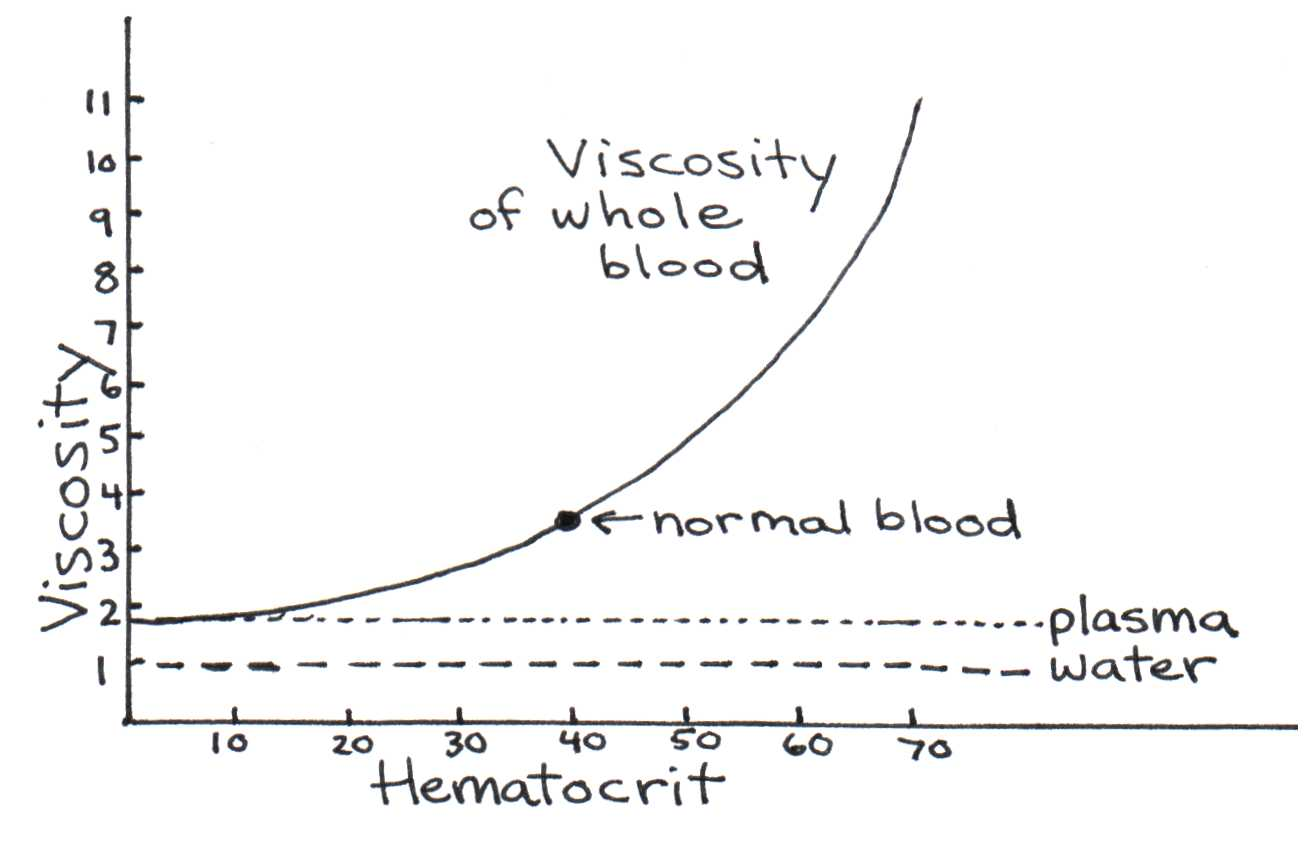
\includegraphics[width=\textwidth]{./figures/Topic2/Fig2-8.jpg}
	\caption{Viscosity’s dependence on the hematocrit.}
	\label{Fig2-9}
\end{figure}
Below a critical diameter of a blood vessel ($\sim$1.5 mm), red blood cells begin to align to pass through the vessel efficiently.  This causes the viscosity to decrease.  The viscosity then increases again in the capillaries, where red blood cells must squeeze through the tiny diameter.
As noted before, blood moves faster in the center of a blood vessel than near the walls.  How can we calculate the velocity of a layer of blood with radius $r$?  Consider a blood vessel of radius $R$ and of length $L$.  If blood is pushed into the vessel by a constant force $F$, we can integrate $dv$ from Eq.~\ref{eqn2-6} (see Appendix A)to show that 
\begin{equation}\label{eqn2-7}
v(r)=\Delta P\frac{R^2-r^2}{4\eta L}
\end{equation}
where $\Delta P$ is the pressure difference from one side of the tube to the other.  The velocity is greatest when $r$ = 0, at the center of the vessel, and decreases parabolically to zero when $r$ = $R$, at the wall of the vessel.  Figure \ref{Fig2-10} illustrates this quadratic dependence.  
\begin{figure}[htbp]
	\centering
	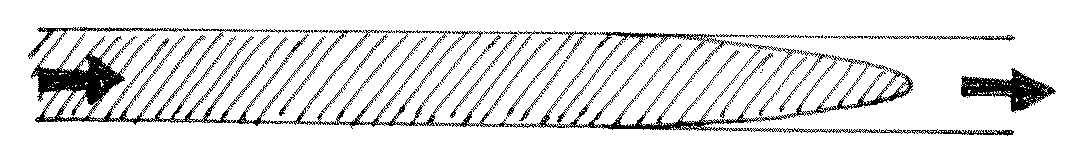
\includegraphics[width=\textwidth]{./figures/Topic2/Fig2-9.jpg}
	\caption{Parabolic blood flow based on Eq.~\ref{eqn2-7}.}
	\label{Fig2-10}
\end{figure}
By integrating the previous equation, we get Poiseuille’s law, which give the volume flow rate of a vessel of radius $R$ and length $L$, taking into account viscosity.
\begin{align}
\frac{dV}{dt} &= \int_0^R v(r) dA\nonumber\\
\frac{dV}{dt} &= \int_0^R v(r)\cdot d\left(\pi r^2\right)\nonumber\\
\frac{dV}{dt} &= \int_0^R v(r)\cdot 2\pi r dr\nonumber\\
\frac{dV}{dt} &= 2\pi \frac{\Delta P}{4\eta L}\int_0^R \left(rR^2 - r^3\right)dr\nonumber
\end{align}
\begin{equation}\label{eqn2-8}
\frac{dV}{dt} = \frac{\pi\Delta P R^4}{8\eta L}
\end{equation}
Note the fourth power dependence of flow rate on radius $R$.  Small changes in the diameter of a blood vessel lead to significant changes in the volume flow rate.  Our bodies take advantage of this sensitive dependence to control the blood supply to tissues. This is accomplished with the use of special muscle tissue surrounding blood vessels that contract or dilate to balance the local demand for blood.  
Thus far, we have considered only the laminar flow of blood, meaning that the fluid moves in smooth, parallel layers.  However, under certain conditions, the flow may become turbulent.  Viscous flow can become turbulent at high Reynold’s numbers.  Reynolds numbers are dimensionless and can be computed using the following equation:
\begin{equation}\label{eqn2-9}
{\rm Re} = \frac{\rho v d}{\eta}
\end{equation}
\[   {\rm flow} = \left\{
\begin{array}{ll}
      {\rm turbulent} & {\rm Re}\leq 3000 \\          
      {\rm unstable} & 2000 < {\rm Re} < 3000 \\
      {\rm laminar} & {\rm Re}\leq 2000 \\
\end{array} 
\right. \]
where $\rho$ is the density and $d$ is the diameter of the blood vessel.  Usually, Re must be greater than about 2000 before the flow becomes turbulent in a smooth vessel. However, turbulence can also be present at lower Reynolds numbers when the fluid passes through a narrowing or when branches into smaller vessels.

Blood flows into the aorta with an average speed of 32 cm/s.  Assuming the diameter of the artery is 2 cm, the viscosity of blood is 0.04 poise, and the density of blood is 1 g/cm$^3$, we estimate the Reynolds number to be 1600, a value critically close to the turbulent limit. Significant levels of turbulence are in fact generated within the aorta if the vessel is narrowed at some point, which can occur when a clot is present. Turbulence can also occur when an aortic valve cannot open fully, forcing the heart to pump blood at a higher velocity into the aorta. Turbulent flow produces a distinct sound that is known in the medical community as a murmur. This sound can be detected with a stethoscope. %Fluids
\setcounter{chapter}{3}
\setcounter{section}{0}
\setcounter{figure}{0}
\setcounter{equation}{0}
\setcounter{table}{0}
\chapter*{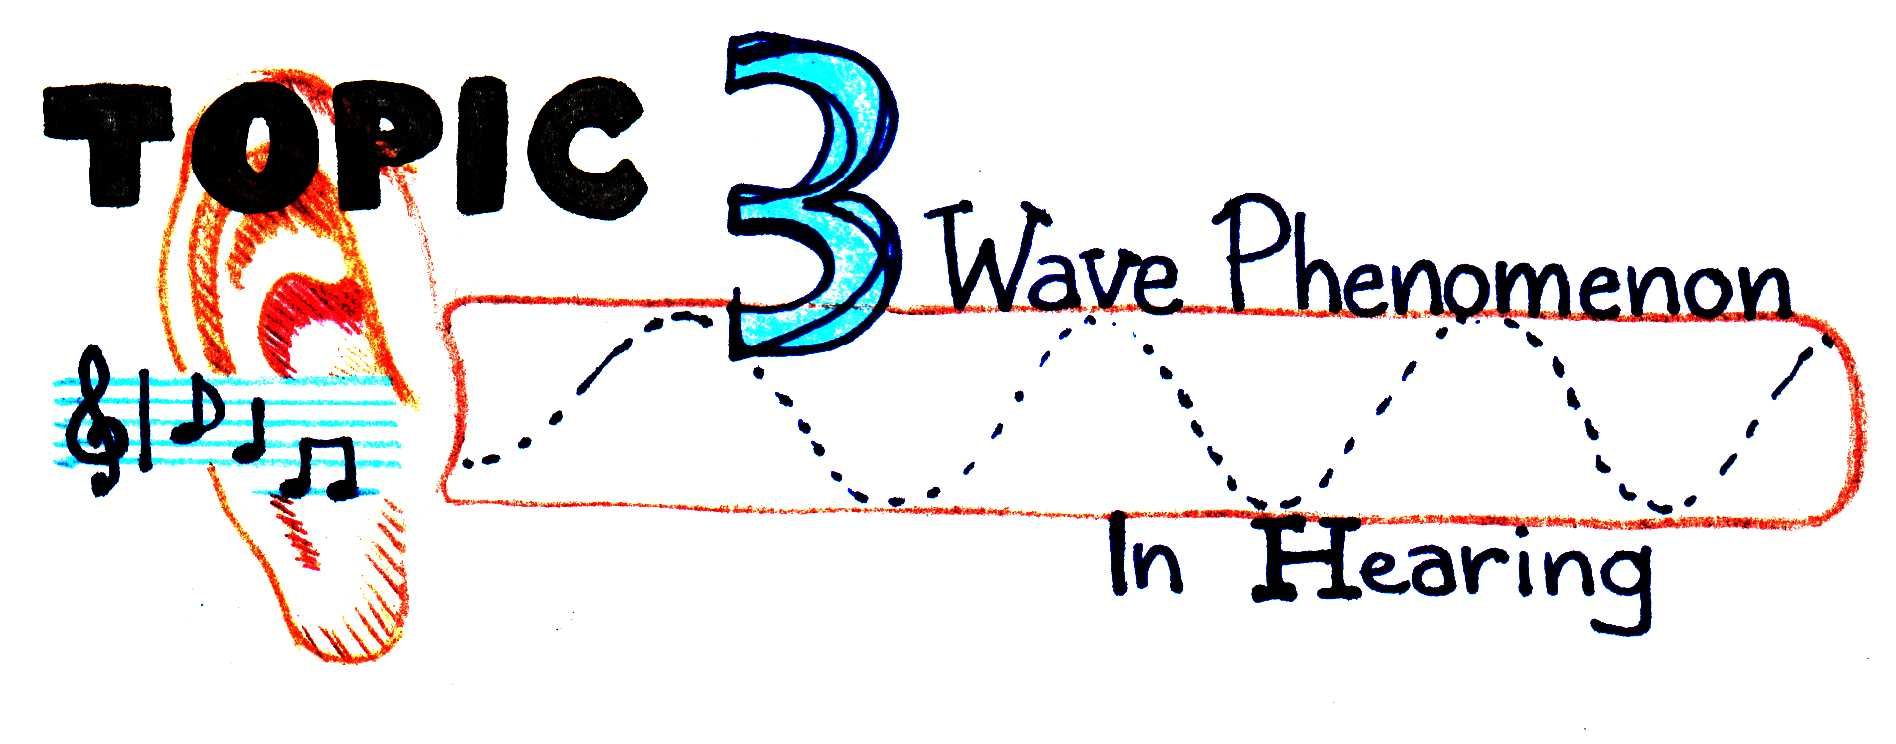
\includegraphics[width=\textwidth]{./figures/Topic3/Topic3.jpg}}
\addcontentsline{toc}{chapter}{Topic 3: Wave Phenomenon in Hearing}

\section{Introduction}

The human ear can detect an extraordinary range of sound intensities, from a faint whisper to a clap of thunder 10 billion times as loud.  The ear can also distinguish frequencies from 20 to 20,000 Hz, allowing us to pick a familiar voice out of a crowd or enjoy the nuances of an aria.  How does the ear perceive such a wide range of sounds, and how is the information transmitted to and integrated in the brain?  
In this chapter, we will first review the physical properties of sound waves and then explore how the ear functions in terms of them.

\section{General Properties of Sound Waves and Hearing}

Sound is a pressure wave traveling in a medium.  We normally consider the medium to be air, but sound travels through liquids and solids as well.  For humans, as noted in the Introduction, the audible range is 20-20,000 cycles per second (Hertz).  Our hearing is particularly well suited to frequencies near 3,700 Hz, which corresponds to human speech.  
\begin{figure}[htb]
	\centering
	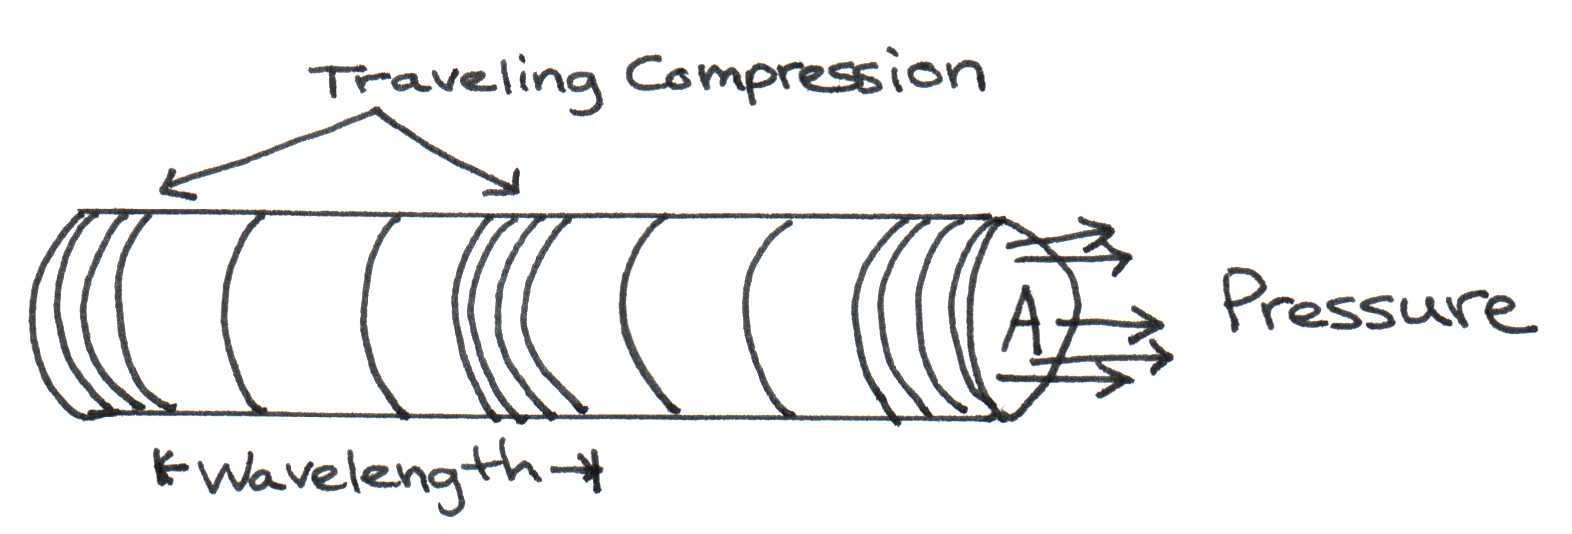
\includegraphics[width=\textwidth]{./figures/Topic3/Fig3-1.jpg}
	\caption{Moving pressure differences.}
	\label{Fig3-1}
\end{figure}
Energy is carried by sound waves in the form of moving pressure differences.  It is important to note that molecules of the medium do not travel the length of the medium with the energy—they transmit the energy by vibrating.   Think of the molecules as a line of people passing along slices of birthday cake at a party.  While the people (the medium) move slightly to do the passing, it is the cake (the energy) that is carried across the room.  For a more accurate analogy of how sound waves propagate, imagine that the medium acts as a slinky.  When the slinky is stretched out, you can create a wave by pinching several rings together at one end and releasing them.  The compression moves along the length of the slinky with a constant speed, c.  As the compression moves past a certain point, energy causes the ring at that point to become displaced by a certain amount in the direction of the wave.  However, the ring stays in the same position relative to the other rings, so only the energy is transmitted.  Similarly, air molecules are pushed together as a sound wave passes, creating a pocket of higher pressure between areas of lower pressure.  It is this compression that gets passed along to adjacent molecules.  Each atom vibrates sinusoidally with a velocity
\begin{equation}\label{eqn3-1}
v(t) = v_o \sin\left(\omega t\right)
\end{equation}
where $v_{\circ}$ is the amplitude of the  velocity of the atom and $\omega$ is its angular frequency, equal to $2\pi$ times the frequency, $f$.  The velocity of an atom, $v$, is not to be confused with the velocity of the wave, c. The speed of sound in air is constant through an air mass of uniform temperature.  We will use c = 350 m/s, which is equivalent to 785 mph.  

The intensity of a sound wave depends on the amount of energy it carries and is related to loudness.  Specifically, intensity measures the work done by the pressure wave per unit time on a surface of area $A$.  Recall that work is the product of force and distance.  If $\Delta x$ is the displacement of a molecule in time period $\Delta t$, then the intensity is
$${\rm Intensity} = \frac{\rm Work~done~by~pressure}{{\rm Area}\cdot{\rm time}}$$
$$I = \frac{W}{A \cdot\Delta t}$$
$$I = \frac{F\cdot \Delta x}{A\cdot t}$$
and since force divided by area is pressure, and $\Delta x$ divided by $\Delta t$ is velocity
\begin{equation}\label{eqn3-2}
I = P v
\end{equation}
where $P$ is the instantaneous pressure as the sound wave passes by, and $v$ is the instantaneous velocity of the atoms driven into oscillation by the pressure.  The magnitude of $P$ is directly related to magnitude of the velocity $v$ of the atoms in the neighboring layer. In fact,
\begin{equation}\label{eqn3-3}
P=\mathcal{Z} v
\end{equation}       

One might expect that lighter atoms/molecules might achieve greater velocities when pushed by the same pressure. Hence the constant $\mathcal{Z}$, which is known as the impedance, must be related to inertia (mass) of the medium. In fact, it can be shown to be the product of the density of the medium, $\rho$, the speed of the sound wave, c, and the area affected sound, $A$.    
\begin{equation}\label{eqn3-4}
\mathcal{Z} = \rho c A
\end{equation}
The concept of impedance is central toward understanding what fraction of sound gets transmitted across the eardrum and into the brain.  We will discuss how this works in a later section.

Sound intensity is sometimes measured in Watts/m$^2$ or Watts/cm$^2$.  The threshold of hearing is approximately 10$^{-12}$ Watts/cm$^2$.  This intensity corresponds to the sound that a mosquito produces several meters away from your ear. To give you another idea of how faint this intensity is, this is equivalent to the intensity of light originating from a 100 Watt incandescent light bulb falling on a 1 cm$^2$ target placed 500 miles away!  At the upper end of the threshold spectrum, the ear detects signals up to 10$^{-6}$ Watts/cm$^2$. The maximum intensity a person can withstand is approximately 100 dB or 10$^{-2}$W/m$^2$.
 
Because the audible range covers ten orders of magnitude, sound is quantified on a logarithmic scale (base 10) rather than on a linear one. See Fig.~\ref{decibels}.
\begin{figure}[htb]
	\centering
	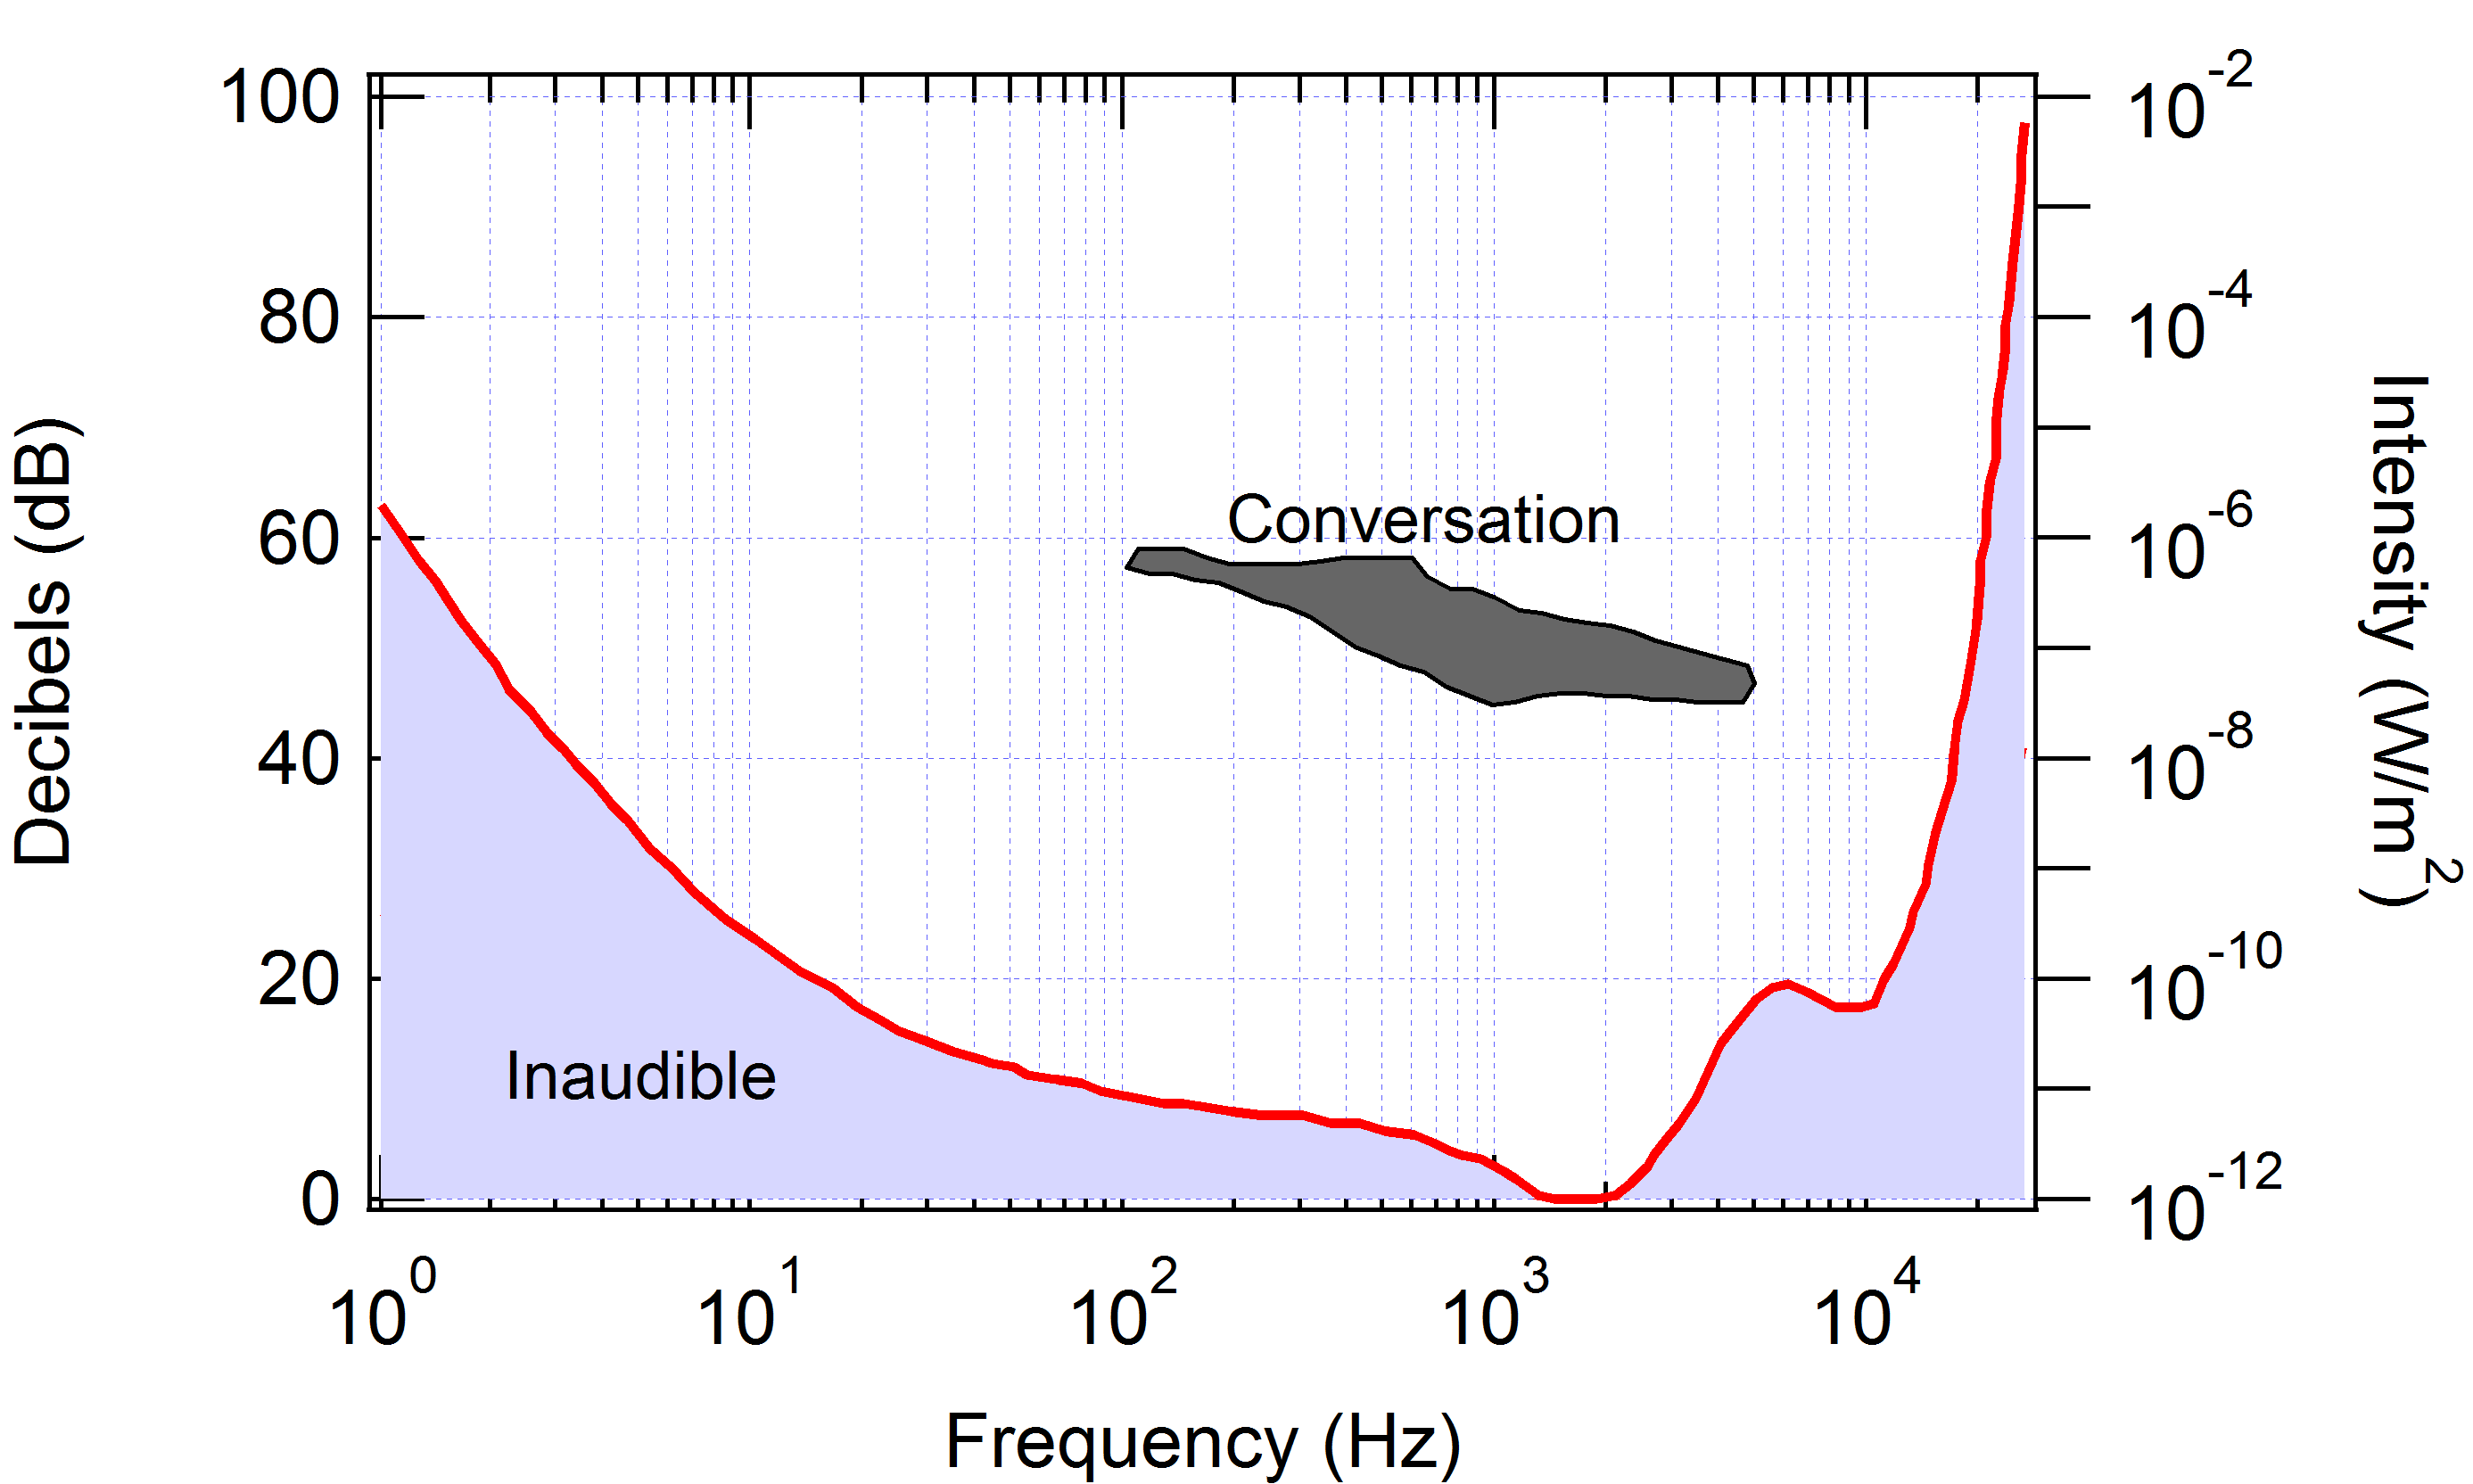
\includegraphics[width=4.5in]{./figures/Topic3/Fig3-decibels.png}
	\caption{Audible threshold vs. frequency. Conversational intensity is shown shaded in the central region of the graph. The lowest audible decibel level is 0 ($I=10^{-12}$W/m$^2$), which occurs at about 2500 Hz.}
	\label{decibels}
\end{figure}
According to this scale, every change in intensity by a factor of ten above some reference level is called a bel.  Usually, the reference level is taken to be the threshold of sound, 10$^{-12}$ W/cm$^2$.  Accordingly, the number of bels for a sound with intensity $I$ relative to this reference level is $\log_{10}\left(I/10^{-12}\right)$.  Often in acoustics, the bel scale is too coarse to quantify loudness.  For this reason, a finer unit is used -- the decibel -- where 1 bel = 10 decibels.  Therefore the sound intensity level in decibels is quantified by the formula
\begin{equation}\label{eqn3-5}
{\rm dB~level} = 10 \log_{10}\left(\frac{I}{10^{-12}}\right)
\end{equation}
Using this scale, one can quantify sound loudness for several sources such as those listed in Table \ref{decibel-table}.
\begin{table}[h]
\begin{center}
\begin{tabular}{|l|c|}
\hline
Source & Loudness (dB) \\
\hline
Whisper & 20--30 \\
Normal conversation & 60--70 \\
Leaf blower near user & 100--110 \\
\hline
\end{tabular}
\caption{Intensity levels in decibels for several common sources of sound.}
\label{decibel-table}
\end{center}
\end{table}

It should be noted that the decibel scale is also used for characterizing changes relative to some arbitrary initial level, i.e. something other than the threshold of hearing. For example, if the sound intensity level is known to increase from some initial level to a final level that is 1000 larger, then one can say that the intensity level increased by 
\begin{eqnarray}\label{eqn3-6}
{\rm dB~change} &=& 10 \log_{10}\left(\frac{I_{\rm final}}{I_{\rm initial}}\right)\\
&=& 10 \log_{10}(1000)\nonumber\\
&=& 30~{\rm dB}\nonumber
\end{eqnarray}

\section{Structure and Function of the Ear}
 
The ear can be divided into three modules (Fig.~\ref{Fig3-2}), each of which performs an important function based on physical principles.  The ear canal, also known as the auditory canal or outer ear, collects sound waves from air and funnels them to the sound-sensing apparatus deep inside the head.  The ear canal, because of its tubular shape, acts as a resonator that allows the ear to hear sound frequencies within the resonance range better than others.  The second module, the middle ear, is designed to increase the transmission of sound waves as they pass from the air to the aqueous fluid of the inner ear, the third module.  The inner ear, in turn, contains sensors that convert water waves into nerve impulses.  The following sections describe the physical principles behind these functions. 
\begin{figure}[h]
	\centering
	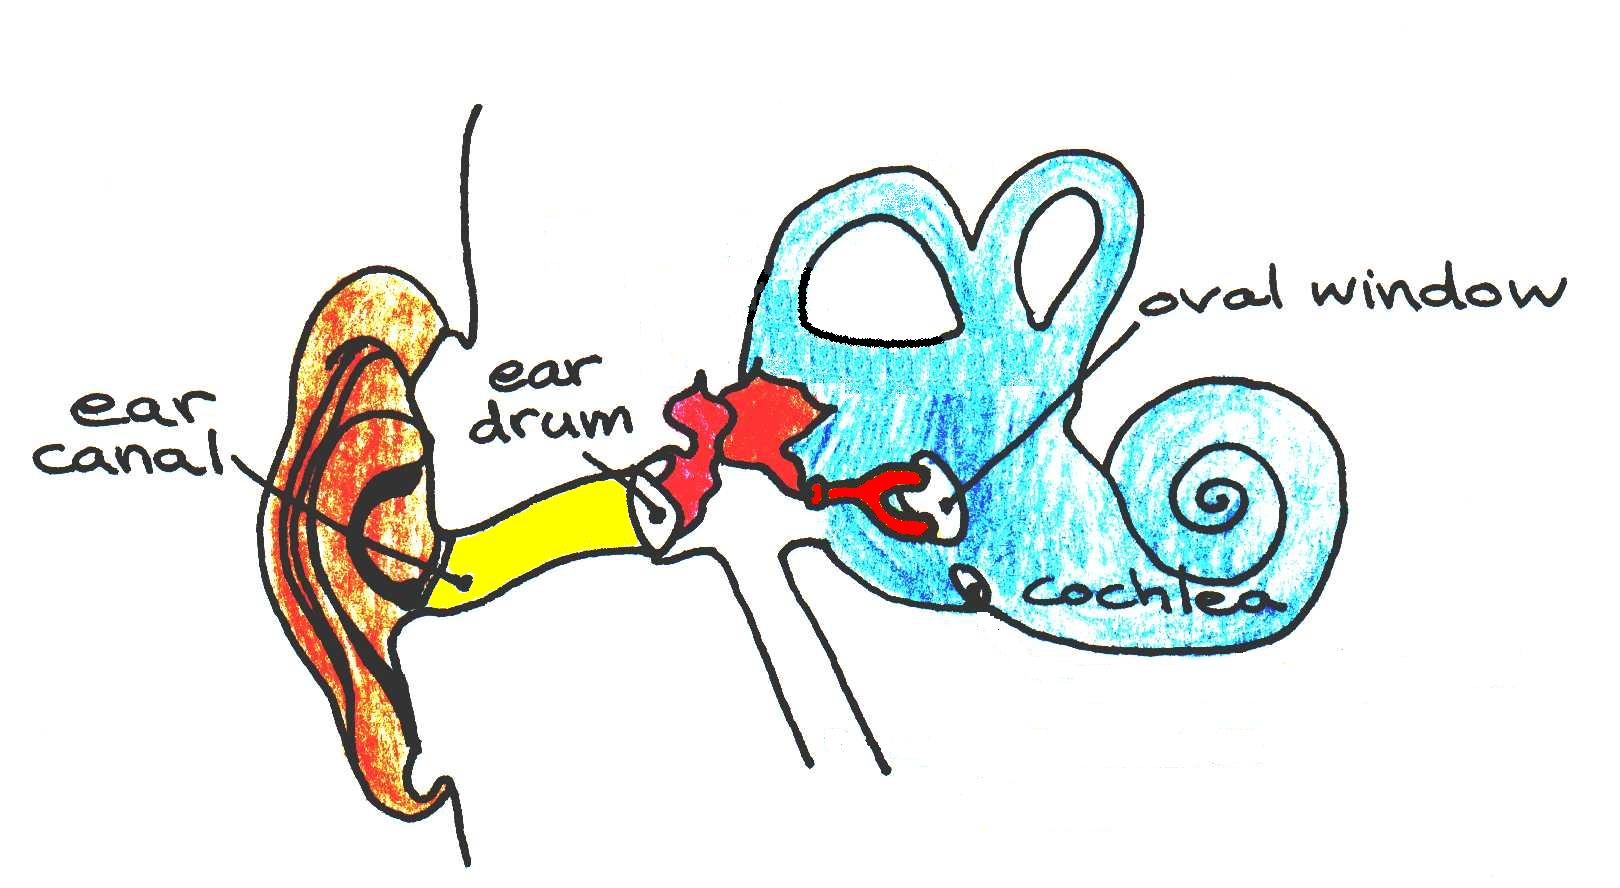
\includegraphics[width=\textwidth]{./figures/Topic3/Fig3-2.jpg}
	\caption{Cross-section of the human ear. The regions filled in yellow, red, and blue correspond to the outer ear (ear canal), the middle ear, and the inner year, respectively.}
 	\label{Fig3-2}
\end{figure}

\subsection{The Auditory Canal}

The outer ear acts as a filter, restricting the passage of certain frequencies to the inner ear.  This performance can be understood in terms of acoustical resonances.  Before proceeding with our discussion, we will first review the principles behind the resonance phenomenon for both closed and opened pipes. Although the closed end case is not pertinent to the discussion of hearing, the equation developed will be useful for a forthcoming discussion of electron resonances within molecules (Topic 6).

\subsubsection{Resonance in a Closed Pipe}

At the closed ends of a pipe, air molecules are unable to vibrate since their motion is blocked by the obstruction that seals the pipe.  Those regions and others where the air does not move are called displacement nodes.  Regions where the pressure does not change are called pressure nodes. In acoustical waves, the displacement is out of step with pressure these regions must correspond to places of maximum pressure. These places are known as pressure anti-nodes.  As you might guess, regions where air molecules move the greatest distance are called displacement anti-nodes.  These points correspond to areas of minimum pressure and are thus also called pressure nodes.  Henceforth, when we speak of nodes and anti-nodes, we will be referring to displacement nodes and anti-nodes, unless otherwise indicated.  

\begin{figure}[htb]
	\centering
	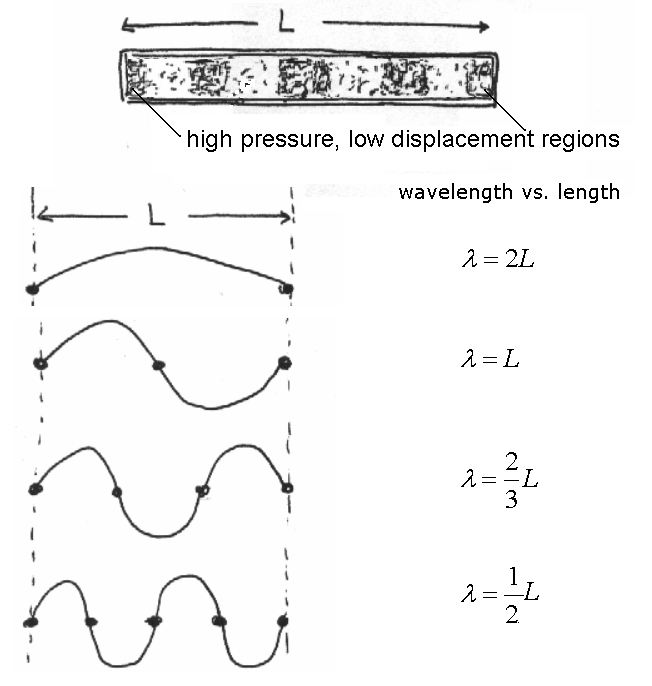
\includegraphics[width=5.0in]{./figures/Topic3/Fig3-3.png}
	\caption{Acoustic patterns inside close-ended pipes.}
 	\label{Fig3-3}
\end{figure}
As shown in Fig.~\ref{Fig3-3}, there are several resonances that can occur inside a closed pipe. The first contains only two nodes at each end and a single anti-node in the middle of the pipe.  In this case, only one half of a full wavelength fits in the pipe.  Thus, for a pipe of length $L$, $\lambda = 2L$.  This is known as the first, or the fundamental, resonance.  If the frequency of the wave increases until there are three nodes and two antinodes, one full wavelength fits in the pipe.  Here, $\lambda = L = (2/2)L$.  Similarly, when there are four nodes, there are three antinodes, and one and a half wavelengths fit in the pipe.  The wavelength changes to $\lambda = (2/3)L$.  We could continue in this same manner forever.  In general, 
\begin{equation}\label{eqn3-7}
\lambda = \frac{2L}{n}
\end{equation}
where $n$ is the number of anti-nodes, always an integer $\geq$ 1. 

\subsubsection{Resonance in a Single Open End Pipe}

The ear canal behaves like a pipe open on one end.  As with the closed pipe, air cannot vibrate at the closed end, so it must be a node.  However, air at the open end is at the same pressure as air outside the pipe, so a pressure node, or a displacement anti-node must be located there.  As shown in Fig.~\ref{Fig3-4}, this means that at the fundamental resonance there is only one node and one anti-node in the pipe. Consequently, only one-fourth of a wavelength fits in the pipe and thus $\lambda = (4/1)L$.  The next resonant pattern corresponds to one with two nodes and two anti-nodes, for which three-fourths of a wavelength fit in the pipe and so $\lambda = (4/3)L$. And the general formula for the pattern becomes 
\begin{equation}\label{eqn3-8}
\lambda = \frac{4L}{2n+1},
\end{equation}
where $n$ = 0, 1, 2, ... ($2n+1 = $~odd integers). Figure $3.5$ below shows the pattern.
\begin{figure}[htb]
	\centering
	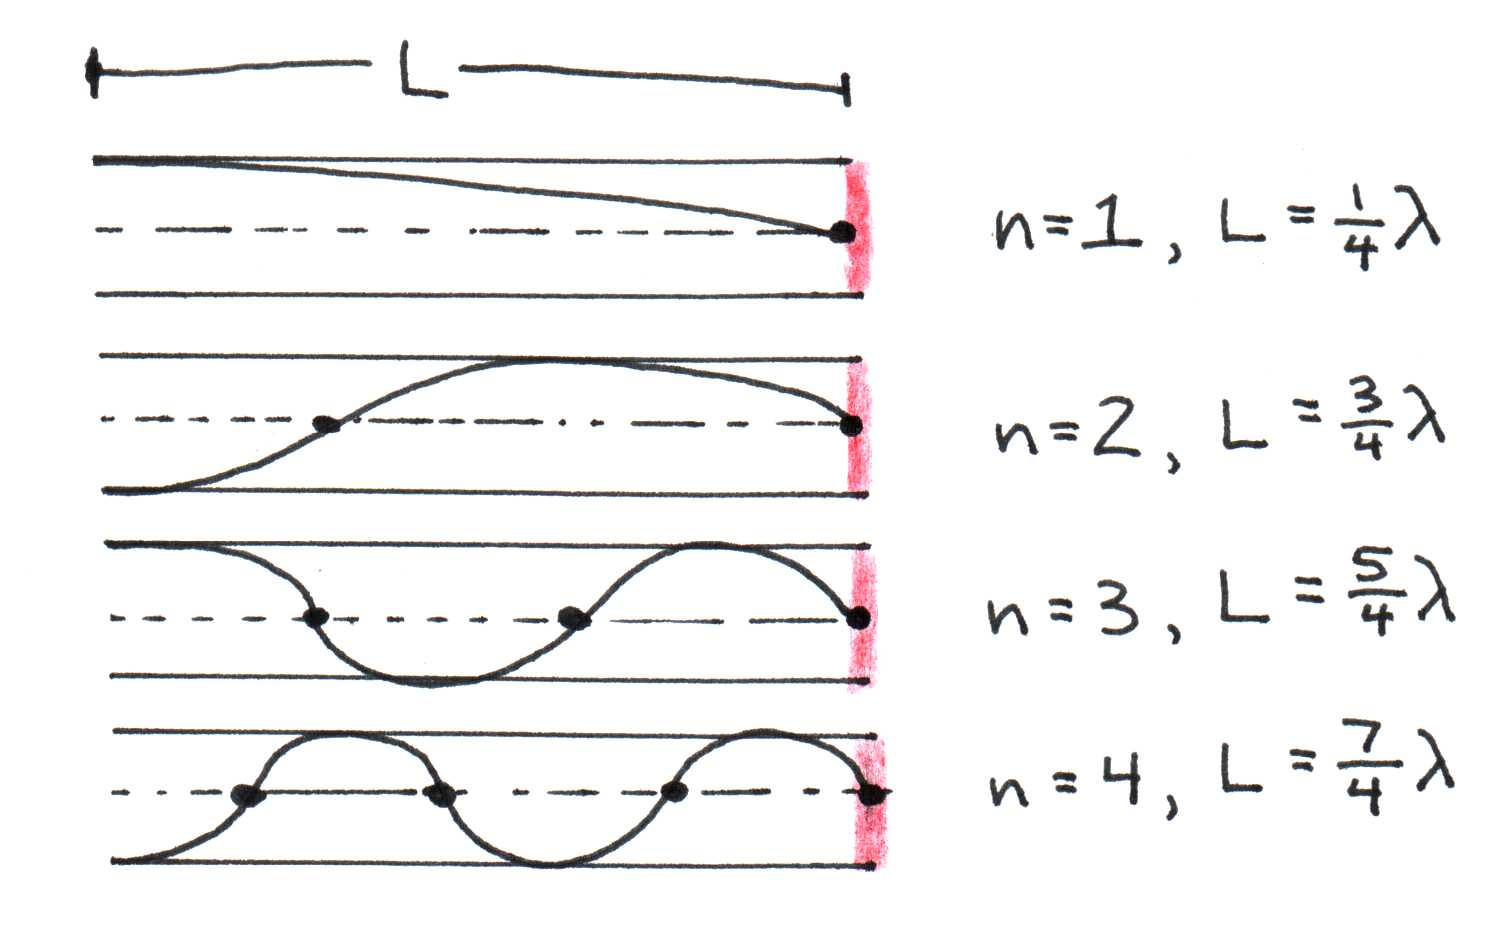
\includegraphics[width=\textwidth]{./figures/Topic3/Fig3-4.jpg}
	\caption{Acoustic resonances in a single open ended pipe.}
	\label{Fig3-4}
\end{figure}
The open-ended pipe model can be used to calculate the resonance frequencies of the human ear.  The lowest frequency at which sound resonates in the ear is found with the above equation where $n$ = 1.  Knowing that c = $\lambda f$, we get c = $4L \cdot f$.  The ear canal is about an inch long, so $L$ = 2.5 cm = 0.025 m.  As noted before, the speed of sound in air is c = 350 m/s.  Using these values, we solve for $f$:
\begin{align}
f &= \frac{c}{4L}\nonumber\\
  &= \frac{350}{4\cdot 0.025}\nonumber\\
  &= 3500~{\rm Hz}\nonumber
\end{align}
In fact, the ear is most sensitive near 3,000 Hz, in agreement with our estimate made above.  The next resonance is predicted to have a frequency three times higher, i.e. 10,500 Hz.  Studies have shown that a small resonance does indeed exist near 12,000 Hz. Notice the increase in sensitivity at this frequency in Fig.~\ref{decibels}. The relation between resonant frequency and the length of the ear canal helps to explain why smaller animals have hearing tuned to higher frequencies, compared to those of larger animals. For instance, the hearing range of mice and rats is between 1000 and 100,000 Hz, while that of an elephant falls between 1 and 20,000Hz.  

\subsection{The Middle Ear}

Sound waves funneled through the auditory canal cause the eardrum to vibrate.  The vibrations are conducted through the three tiny bones (collectively called the ossicles) of the middle ear to their point of contact on the cochlea (inner ear) known as the oval window.  These bones serve two purposes: they protect against loud noises through the attenuation reflex, and they provide what is known as impedance matching between the outer ear and inner ear.  The attenuation reflex occurs when muscles reduce the action of the ossicles in response to a harmfully loud noise.  The physics of impedance matching will be discussed in depth in the following section.

\subsubsection{Impedance Matching}

When sound waves traveling in air collide with the surface of another medium, like water, they are mostly reflected.  Only a fraction of the wave’s energy is transmitted to the target medium.  You might have experienced this while swimming -- if someone tries to speak to you while you are under water, you will be unable to hear the person, because the sound waves bounce off the surface of the pool.  This phenomenon can be explained in terms of the conservation laws of momentum and energy.  Recall from Fig.~\ref{Fig3-1} that it is the pressure changes associated with a sound wave that propels a pocket of molecules to move through the air.  When one of these pockets of air traveling with a velocity $v_{a1}$ collides with a stationary mass of water ($v$ = 0), the collision is essentially elastic, meaning that no kinetic energy is lost.  Some of the air’s kinetic energy is transferred to the water mass, so that the air mass bounces off with velocity $v_{a2}$ and the water mass moves with velocity $v_{w}$.  This is depicted in Figure \ref{Fig3-5} below.
\begin{figure}[htb]
	\centering
	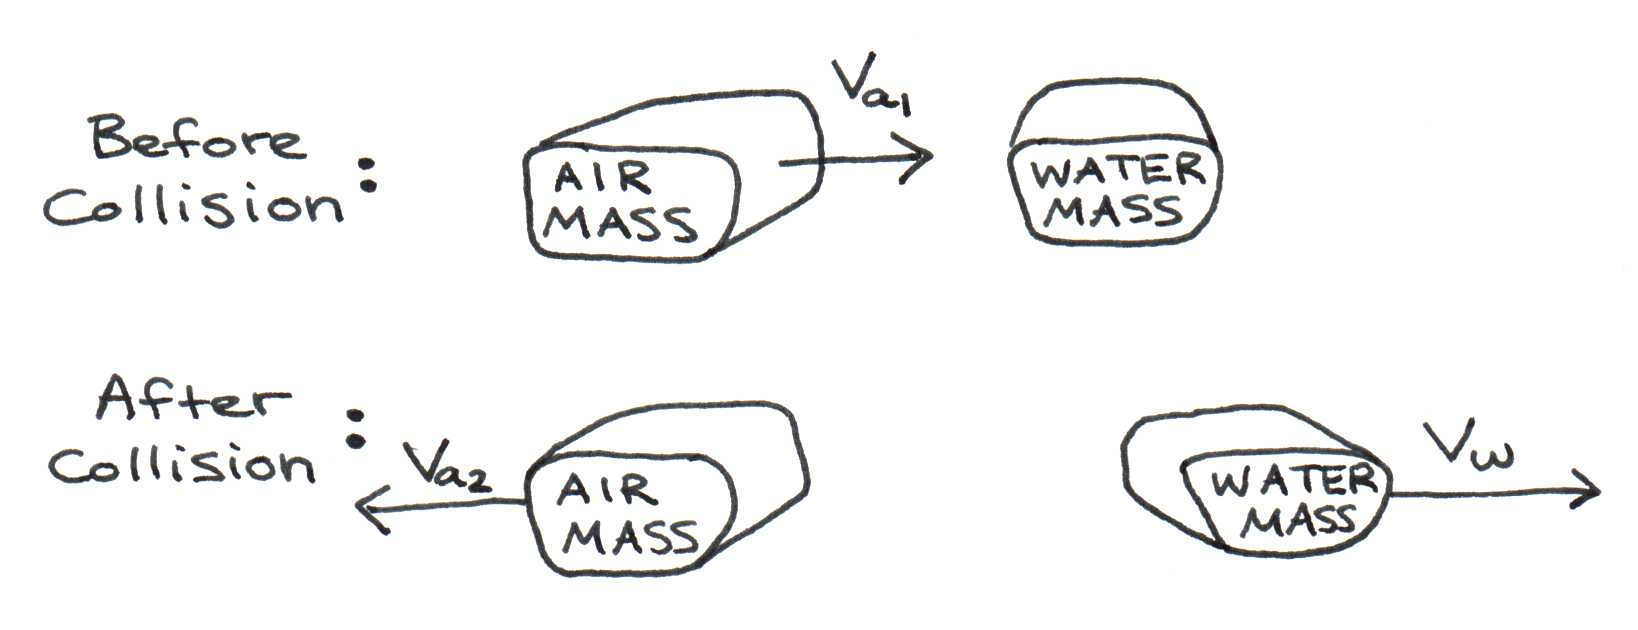
\includegraphics[width=5.0in]{./figures/Topic3/Fig3-5.jpg}
	\caption{Collision of an air mass (pressure pocket) with a stationary water mass.}
 	\label{Fig3-5}
\end{figure}
 
According to the conservation laws,
\begin{align}
m_av_{a1} &= m_av_{a2} + m_wv_w &{\rm Momentum}\nonumber\\
\frac{1}{2}m_av_{a1}^2 &= \frac{1}{2}m_av_{a2}^2 + \frac{1}{2}m_wv_w^2 &{\rm Energy}\nonumber
\end{align}
(Note that these velocities are related to the ones described by Eq.~\ref{eqn3-1}-- {\bf none} is the same as the speed of sound c in either media).  By solving this system of equations, one can show that
\begin{equation}\label{eqn3-9}
	v_{a2}=\frac{m_a-m_w}{m_a+m_w}v_{a1}
\end{equation}
\begin{equation}\label{eqn3-10}
	v_w=\frac{2m_a}{m_a+m_w}v_{a1}
\end{equation}
The energy transmission $T$ is defined as the ratio of the energy transmitted through the water over the energy incident on the water.  Substituting Eqs.\ref{eqn3-9} and \ref{eqn3-10}, we obtain the following equation:
\begin{eqnarray}\label{eqn3-11}
T &=& \frac{\frac{1}{2}m_wv_w^2}{\frac{1}{2}m_av_{a1}^2}\nonumber\\
&=& \frac{\frac{1}{2}m_w\left(\frac{2m_a}{m_a+m_w}v_{a1}\right)^2}{\frac{1}{2}m_av_{a1}^2}\nonumber\\
&=& \frac{4 m_a m_w}{\left(m_a+m_w\right)^2}\nonumber\\
&=& \frac{4 m_w/m_a}{\left(1+m_w/m_a\right)^2} 
\end{eqnarray}
Next we demonstrate that the masses $m_a$ and $m_w$ are related to the concept of acoustical impedance we discussed earlier. To do so, it is helpful to visualize first how these masses relate to the concept of wavelength in the medium. Recall from Fig.~\ref{Fig3-1} that the pressure change during half of the acoustic cycle propels forward a layer of molecules about $1/2\lambda$ thick. This shown below in Fig.~\ref{Fig3-6} more explicitly. 
\begin{figure}[htb]
	\centering
	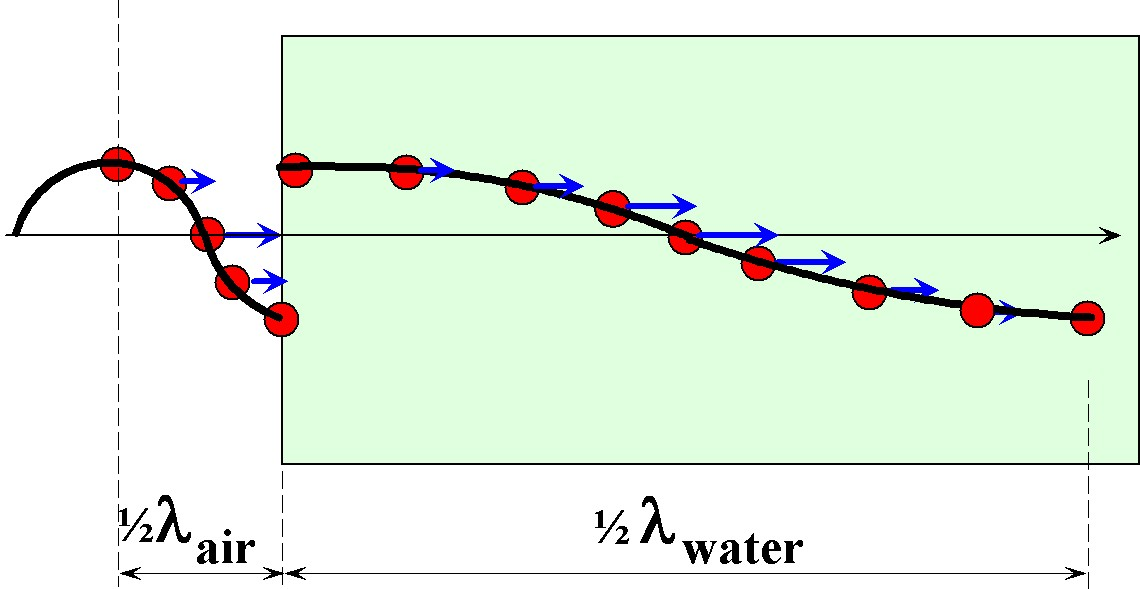
\includegraphics[width=5in]{./figures/Topic3/Fig3-6.jpg}
	\caption{A look at half a wavelength in media of different densities.}
 	\label{Fig3-6}
 \end{figure}
The mass propelled forward by the pressure spike can therefore be visualized as a rectangular volume with a length$1/2\lambda_a$ and a cross-sectional area $A_a$ perpendicular to the length. The mass of air $m_a$ is therefore 
\begin{equation}\label{eqn3-12}
m_a = \rho_a \frac{\lambda}{2}A_a
\end{equation}
Since the wavelength can be expressed in terms of speed of sound c and the frequency $f$ ($\lambda_a=c_a/f$), the mass $m_a$ can be expressed as 
\begin{equation}\label{eqn3-13}
m_a = \frac{\rho_a c_a A_a}{2f}
\end{equation}
Similarly, the mass of the water that the air collides with is 
\begin{equation}\label{eqn3-14}
m_w = \frac{\rho_w c_w A_w}{2f}
\end{equation}
where $A_w$ is the area of the water that is pushed.  
Substituting Eqs.~\ref{eqn3-13} and \ref{eqn3-14} into Eq.\ref{eqn3-11}, we see that 
\begin{equation}\label{eqn3-15}
T = \frac{4\rho_w c_w A_w/\rho_a c_a A_a}{\left(1+\rho_w c_w A_w/\rho_a c_a A_a\right)^2}
\end{equation}
What if the middle ear did not exist, that is, what if air waves struck the fluid in the inner ear directly?  Then $A_a$ would equal $A_w$.  Given that $\rho_w/\rho_a$ = 800/1 and $c_w/c_a$ = 5/1 when the medium $a$ is air and the medium $w$ is water,
$$T = \frac{4\cdot 800\cdot 5\cdot 1}{\left(1+800\cdot5\cdot1\right)^2} = 0.001$$
A 0.1\% transmission corresponds to a transmission level that is 1000 times smaller than the initial level. According to Eq.~\ref{eqn3-6}, the corresponding decibel change is
\begin{eqnarray}
{\rm dB~change} &=& 10 \log_{10}\left(\frac{I_{\rm final}}{I_{\rm initial}}\right)\nonumber\\
&=& 10 \log_{10}\frac{1}{1000}\nonumber\\
&=& -30~{\rm dB}\nonumber
\end{eqnarray}
or a loss of 30 decibels. This is the equivalent of a loud concert becoming a whisper.

The transmission can also be written in terms of impedance.  Recall Eq.~\ref{eqn3-4}, which states that impedance $\mathcal{Z} = \rho cA$.  Eq.~\ref{eqn3-11} becomes
\begin{equation}\label{eqn3-16}
T = \frac{4\mathcal{Z}_w/\mathcal{Z}_a}{\left(1+\mathcal{Z}_w/\mathcal{Z}_a\right)^2}
\end{equation}
Fig.~\ref{Fig3-7} plots how the transmission depends on the impedance ratio, according to Eq.~\ref{eqn3-16}.  To get 100\% transmission, $\mathcal{Z}_a$ must equal, or match, $\mathcal{Z}_w$.  This is why impedance matching is so important to maximize transmission.  
 \begin{figure}[h]
	\centering
	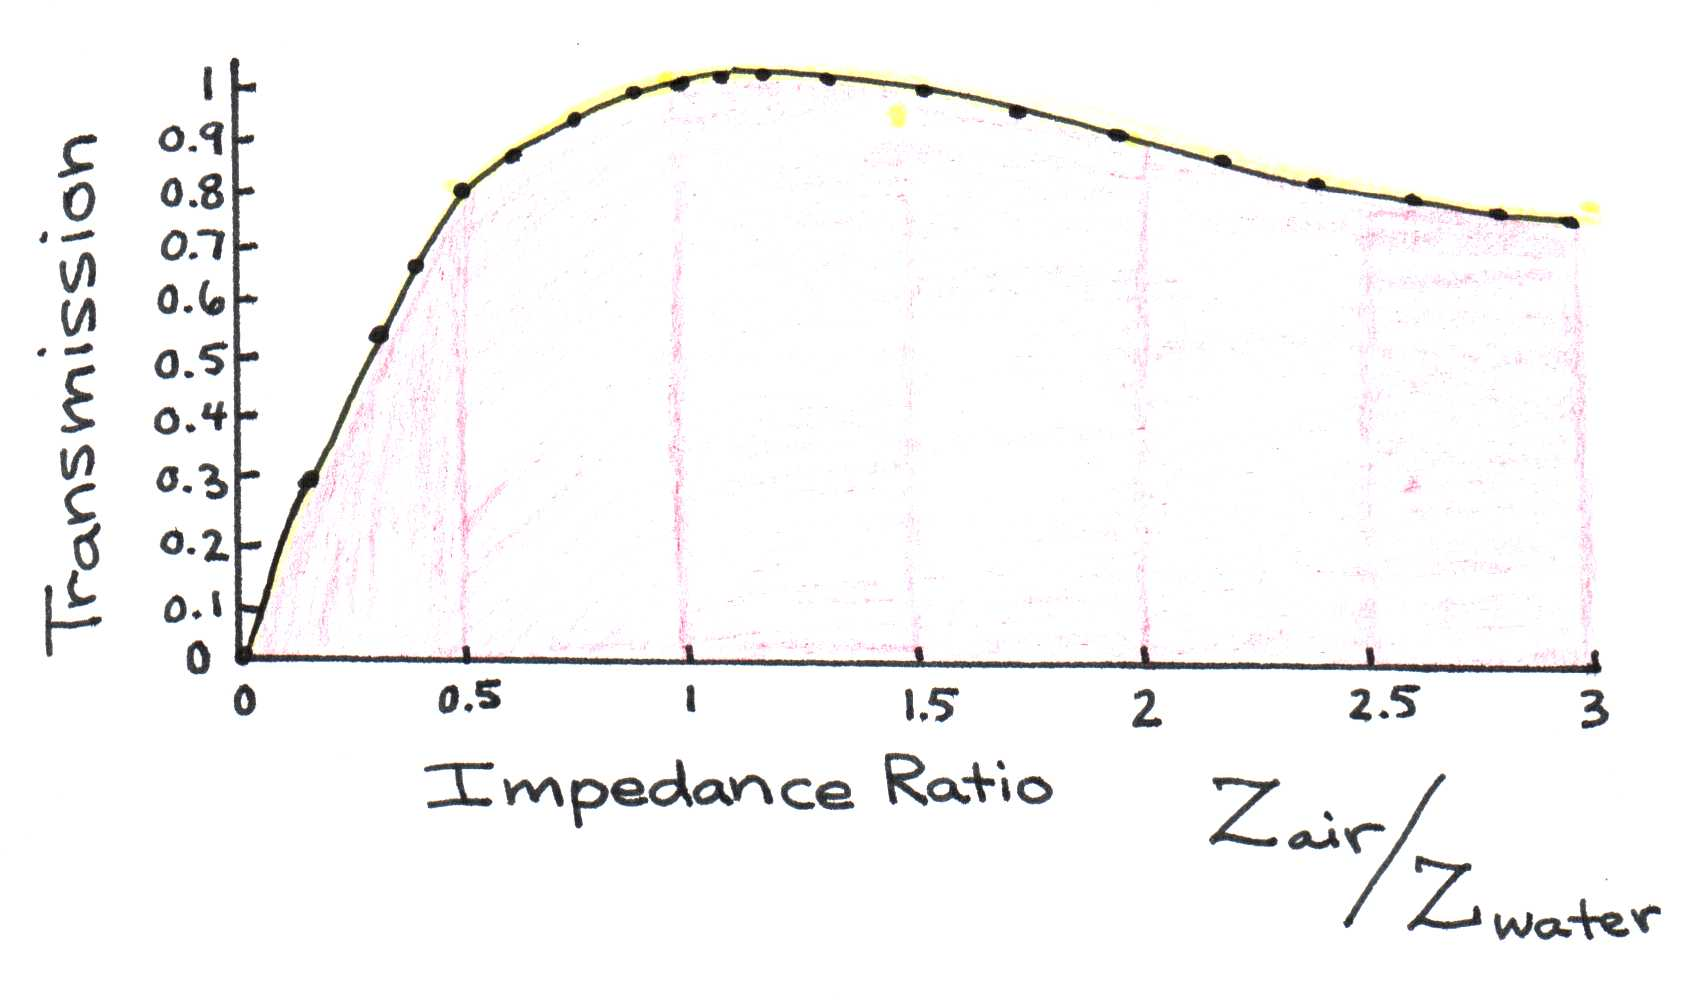
\includegraphics[width=5in]{./figures/Topic3/Fig3-7.jpg}
	\caption{Dependence of transmission on impedance ratio.  Note that transmission is 100\% effective only when the impedances are equal.}
 	\label{Fig3-7}
 \end{figure}  
So what would happen if the middle ear was not present, and sound waves struck directly the oval window of the fluid-filled inner ear? In that case the sound transmission would diminish by 30 decibels as our calculations predict. Fortunately, our hearing has evolved a way to minimize the impact of impedance mismatch at the interface between air and water. Sound waves traveling through air strike the surface $A_{eardrum}$ of the ear drum. This acoustical power is then channeled through the middle ear bones into a much smaller area focused around the oval window. The ratio of the areas $A_{eardrum}/A_{oval-window}$ results in a ratio $A_a/A_w\approx 20$ in Eq.~\ref{eqn3-14}, rather than 1 as we assumed without the middle ear. In terms of impedance, the mismatch between $\mathcal{Z}_a$ and $\mathcal{Z}_w$ ($\mathcal{Z}_a$/$\mathcal{Z}_w$ = 1/4000) is now significantly reduced ($\mathcal{Z}_a$/$\mathcal{Z}_w$ = 20/4000), allowing the sound transmission into the inner ear to increase approximately 20 fold.  The function of the middle ear is thus to aid in impedance matching. 

\subsection{The Inner Ear}

The part of the inner ear used in hearing is called the cochlea (Latin for ``snail shell'').  This complex structure contains a coiled set of tubes, the inner structure of which is shown in greater detail in Figure \ref{Fig3-8}.  
 \begin{figure}[htb]
	\centering
	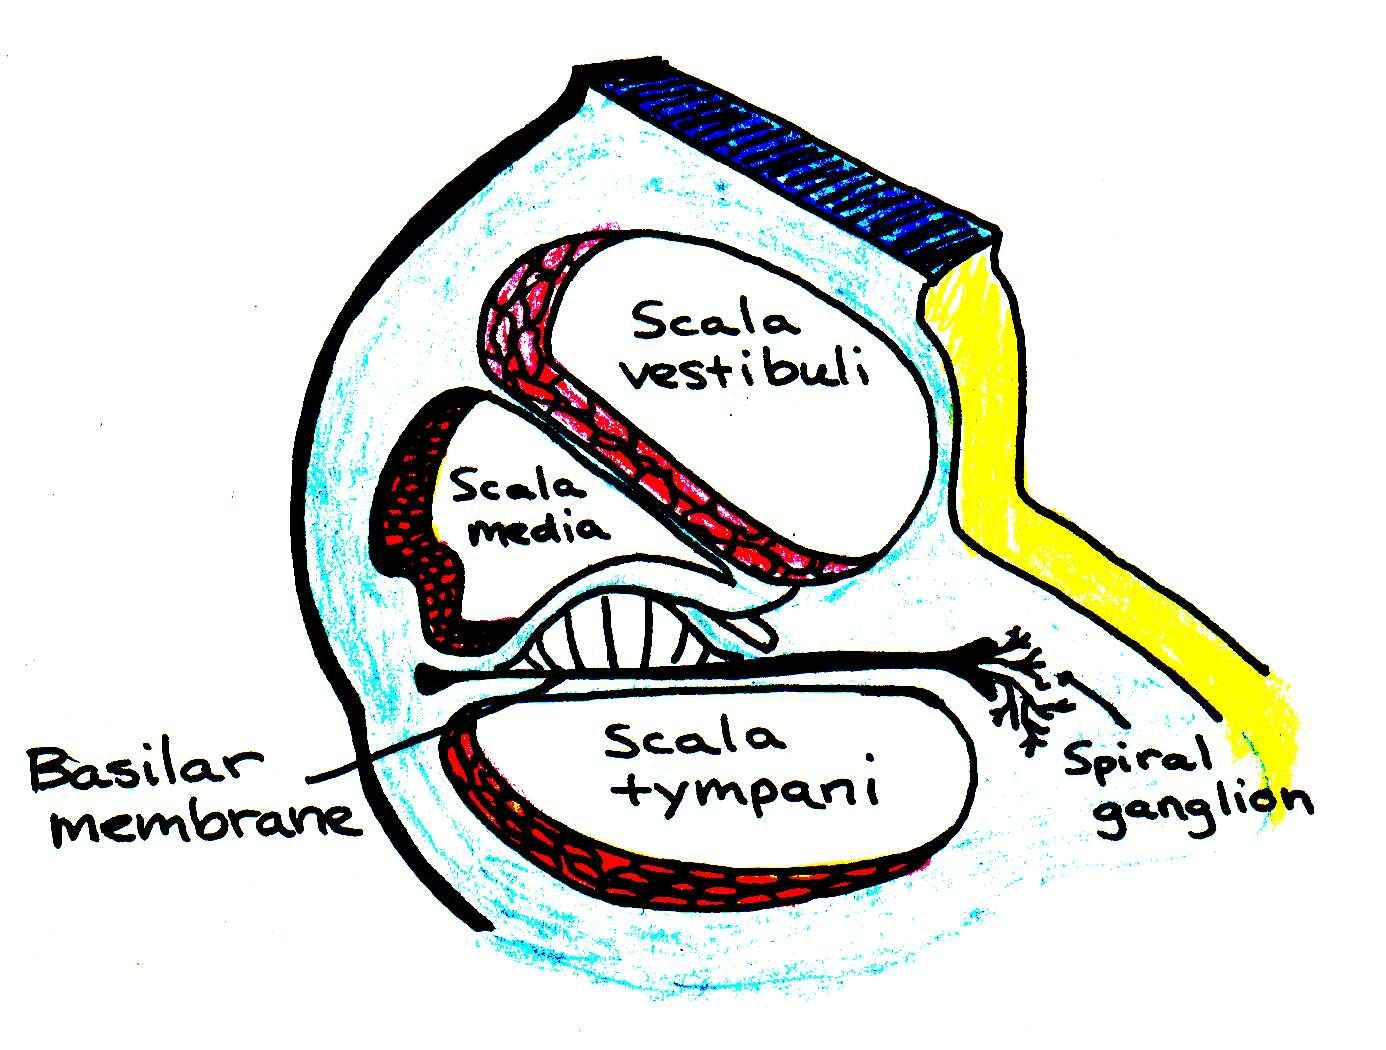
\includegraphics[width=5in]{./figures/Topic3/Fig3-8.jpg}
	\caption{Cross-section through one of the turns of the cochlea. }
 	\label{Fig3-8}
\end{figure}   
The conversion of acoustic signals to nerve impulses takes place in the cochlea, specifically at hair cells located in the space between the scala tympani and the scala vestibuli.  When the stapes (stirrup) cause the oval window to vibrate, a traveling pressure wave is created in the cochlear fluid.  The basilar membrane, which extends along the length of the cochlea, vibrates in response to the pressure wave.  
\begin{figure}[htb]
	\centering
	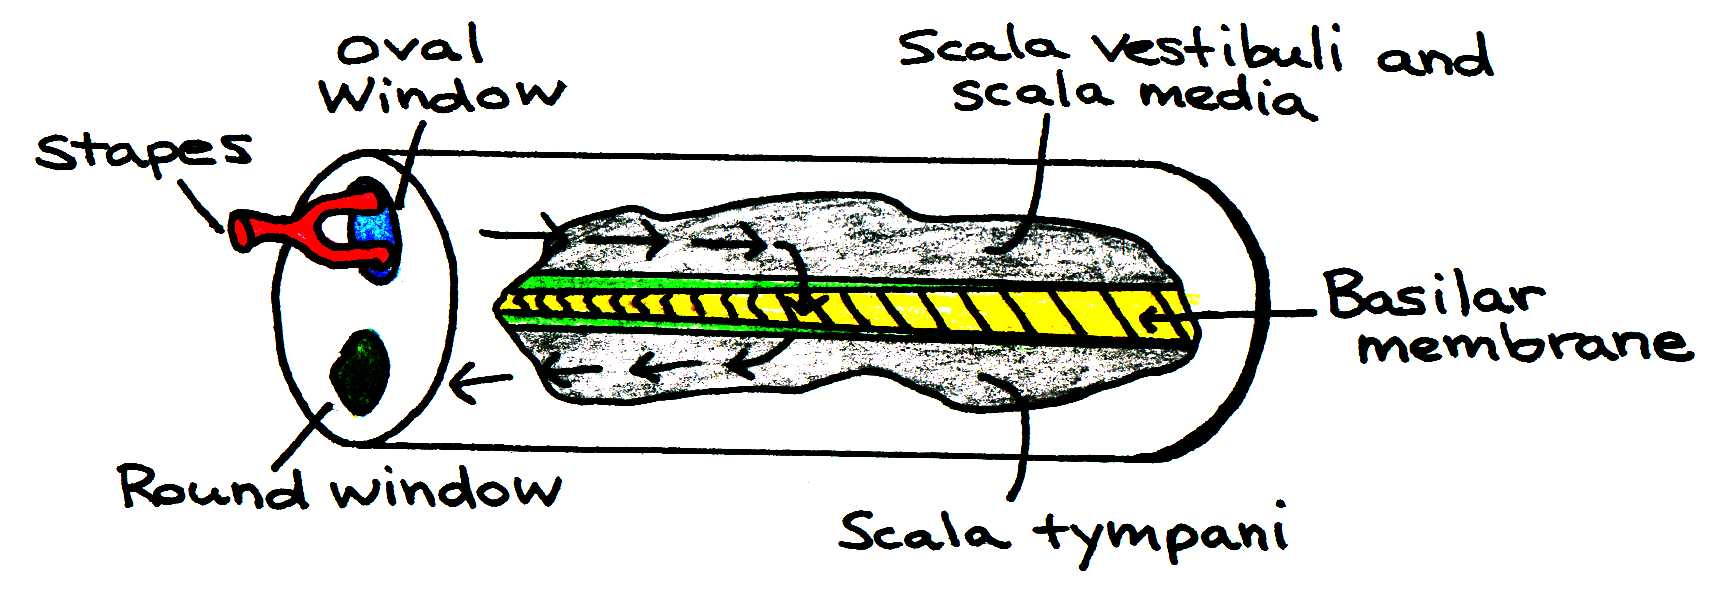
\includegraphics[width=\textwidth]{./figures/Topic3/Fig3-9.jpg}
	\caption{Movement of fluid in the cochlea.}
 	\label{Fig3-9}
\end{figure}
Basilar fibers, which vary in length and stiffness along the basilar membrane, respond to the wave by bending back and forth.  See Fig.~\ref{Fig3-10}. Movement of these fibers causes hair cells in the immediate vicinity to vibrate, which triggers nerve impulses that travel to the brain and are interpreted as a sound of a particular frequency. The function of the inner ear relies heavily on the resonance phenomenon. We will now model the physics of resonance in basilar fiber motion.  

\subsubsection{Resonance in Basilar Fiber Motion}

Consider a simple elastic system that is allowed to oscillate, as shown in Figure \ref{Fig3-10}, where $k$ is the elastic constant.  
 \begin{figure}[htb]
 	\centering
	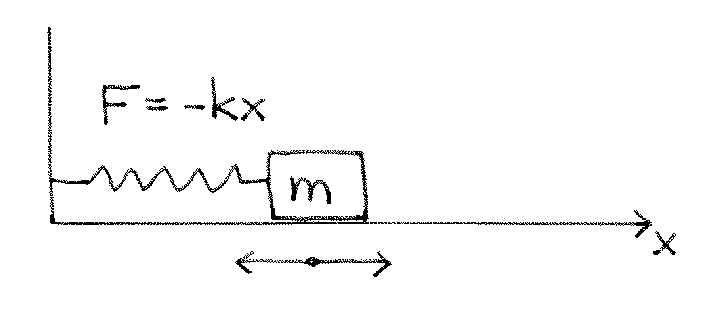
\includegraphics[width=5in]{./figures/Topic3/Fig3-10.jpg}
	\caption{A simple elastic system.}
 	\label{Fig3-10}
 \end{figure}
Applying Netwon’s 2nd law of motion,
\begin{eqnarray}\label{eqn3-17}
	\sum F_x &=& ma\nonumber\\
	-kx &=& m \frac{d^2x}{dt^2}\nonumber\\
	\frac{d^2x}{dt^2} &=& -\frac{k}{m}x 
\end{eqnarray}
This differential equation is very similar to the one obtained in the pendulum problem in Topic 1.  The solution to this equation is 
 \begin{equation}\label{eqn3-18}
	 x(t) = A \sin\left(\sqrt{\frac{k}{m}}t\right)
 \end{equation}
Letting $T\sqrt{k/m} = 2\pi$, we find that the period $T=2\pi\sqrt{m/k}$. The resonant frequency of the system associated with this vibration is therefore
$$f_{\circ}=\frac{1}{T} = \frac{1}{2\pi}\sqrt{\frac{k}{m}}$$

The basilar fibers in the inner ear behave like reeds.  Reeds vibrate with a certain frequency since they are free to oscillate.  They have a stiffness $k$ and some inertia $m$.  As mentioned before, the length of the basilar fibers is not uniform.  Near the stapes, they are 0.04 mm, increasing steadily with distance from the stapes to a length of 0.5 mm.  At the same time, the stiffness of the fibers decreases by a factor of 100.  Both of these factors contribute to a significant change in the ratio $k/m$, which affects the resonant frequency of the fibers.

The frequency of the incoming traveling wave determines how deep the wave penetrates the cochlea.  High-frequency waves resonate best at the short, stiff fibers near the stapes, so the sound is absorbed there.  Low-frequency waves travel much farther along the basilar membrane before being absorbed by the longer, more flexible fibers.  Figure \ref{Fig3-11} illustrates this fact.  
\begin{figure}[htb]
	\centering
 	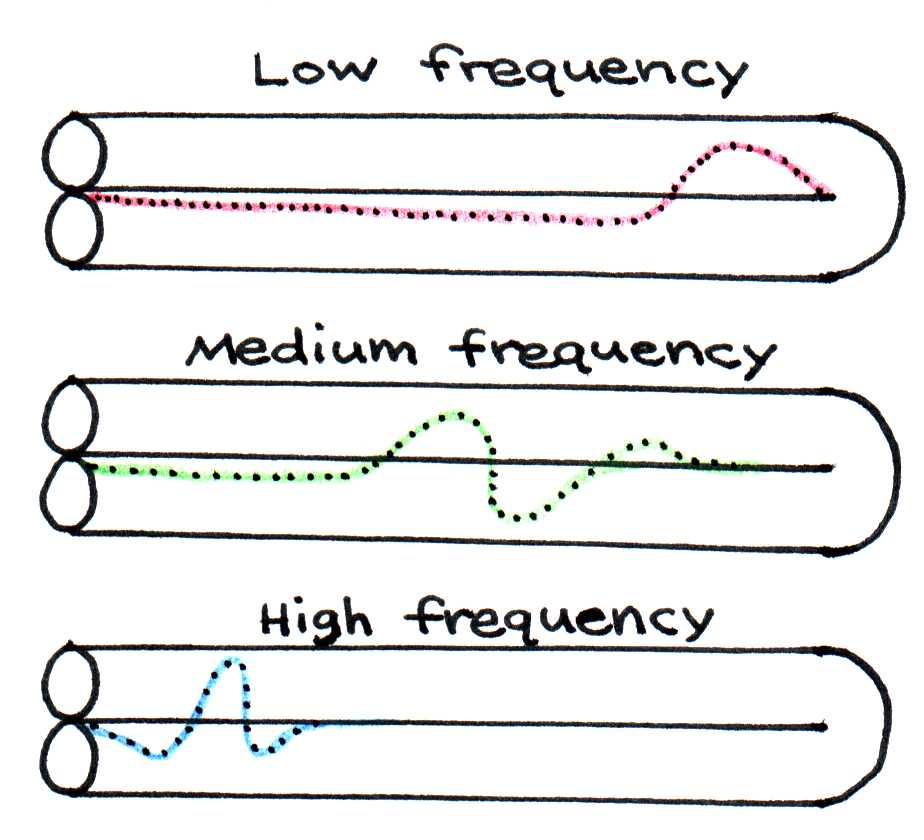
\includegraphics[width=4.5in]{./figures/Topic3/Fig3-11.jpg}
 	\caption{Traveling waves along the basilar membrane.}
	\label{Fig3-11}
\end{figure}
 
The basilar fibers allow us to distinguish the loudness and pitch of a sound.  A wave with a large amplitude causes the fibers to vibrate vigorously.  In response, action potentials are rapidly created, and the brain interprets this as a loud sound.  A sound wave with a high frequency, on the other hand, causes hair cells adjacent to a point on the basilar membrane near the oval window to vibrate.  This stimulates neurons to fire signals to the brain that are interpreted as a high pitch. %Hearing
\setcounter{chapter}{4}
\setcounter{section}{0}
\setcounter{figure}{0}
\setcounter{equation}{0}
\setcounter{table}{0}
\chapter*{
\includegraphics[width=\textwidth]{./figures/Topic4/Topic4.jpg}}
\addcontentsline{toc}{chapter}{Topic 4: Heating and Cooling of the Body}

\section{Introduction}

Thermoregulation is the maintenance of body temperature within a range at which cells can function effectively.  Although various species have adapted differently, each is suited to an optimal temperature range.  Each animal has physical and behavioral adaptations that allow it to maintain a constant internal temperature, regardless of fluctuations in the ambient (external) temperature.  
Body temperature on the skin’s surface is much lower than the temperature of tissues deep inside the body -- the so-called ``core temperature.''  For humans, the core temperature is normally between 98$^{\circ}$F and 98.6$^{\circ}$F (measured orally).  Even when exposed for several hours to ambient temperatures between 60$^{\circ}$F and 130$^{\circ}$F, our core temperature varies little -- from 97$^{\circ}$F to 100$^{\circ}$F.  Figure \ref{Fig4-1} illustrates this stability of the core temperature.
\begin{figure}[h]
	\centering
	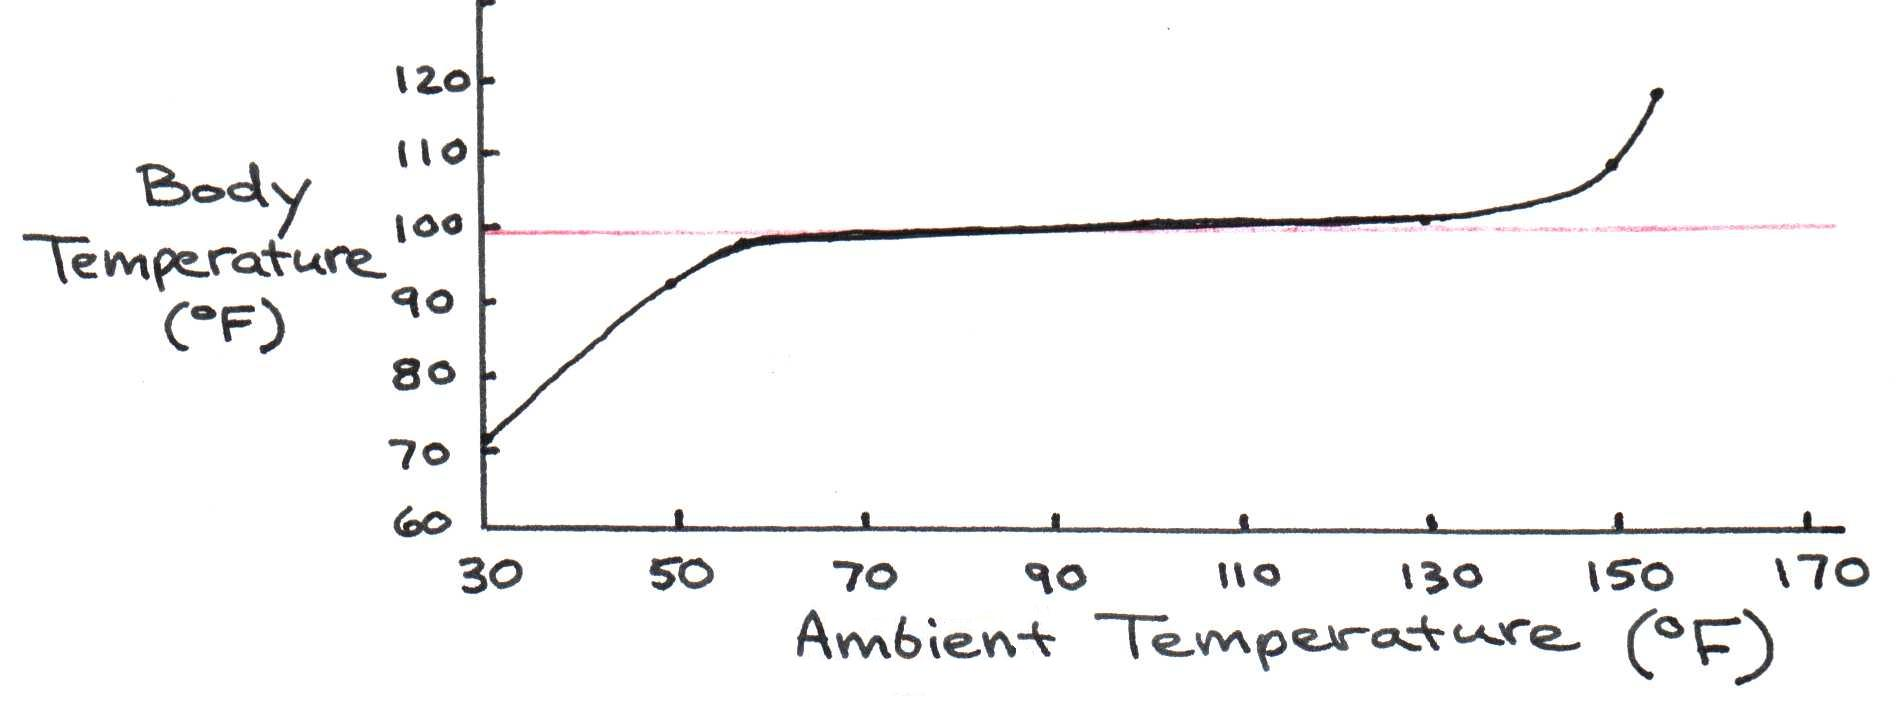
\includegraphics[width=\textwidth]{./figures/Topic4/Fig4-1.jpg}
	\caption{Effect of ambient temperature on internal body temperature.  Note the stability of the core temperature despite wide variations in atmospheric temperature.}
	\label{Fig4-1}
\end{figure}  

How do we accomplish thermoregulation?  A portion of our brain known as the hypothalamus controls a number of mechanisms that balance heat production with heat dissipation.  We will first discuss how heat is produced through metabolic activity and then investigate the ways in which heat is dissipated into the environment.
  
\section{Heat Production}

Unlike cold-blooded animals (ectotherms), which warm their bodies by absorbing heat from their environment, humans and other endotherms generate heat from chemical reactions in the body.  These chemical reactions (see Appendix B), collectively referred to as metabolism, are generally inefficient, releasing over 75\% of their energy as heat.
 
This internal generation of heat is particularly noticeable during fever, which is a natural immune response to invading pathogens. When the hypothalamus receives chemical signals characteristic of invading pathogens it increases metabolism, which is partially responsible for the increased temperature of the body. Metabolism also increases during strenuous exercise.  As muscles work hard, cells require more energy and thus must increase their rate of respiration.  Cellular respiration is the process of using oxygen and complex food molecules to create ATP, a molecule often dubbed the cell’s ``energy currency.''  So much internal heat is created from these reactions that under moderate ambient temperatures, the core temperatures can rise to 102$^{\circ}$F or 103$^{\circ}$F.  In hot weather, the core temperature can rise to a dangerous 106-108$^{\circ}$F during exercise.
The basal metabolic rate (BMR) for an endotherm is defined as the baseline rate of metabolism with no muscle activity, on an empty stomach, and with no stress.  Many factors can influence the BMR, including age, sex, body size, body temperature, ambient temperature, quality and quantity of food, and activity level.  For humans, the average BMR is approximately 60 kcal/hour for young adult males and 53 kcal/hour for young adult females.  (While we often speak of “counting calories,” the amounts of energy listed on nutritional information labels are actually measured in kilocalories, where 1 kilocalorie (kcal or C) = 1,000 calories.  Also, 1 kcal = 4,186 J.  Just to maintain the BMR, males must consume 1,600-1,800 kcal per day and females must consume 1,300-1,500 kcal per day.  Eating and digesting increases daily caloric expenditure by 200 kcal, while sitting adds another 200 kcal.  Depending on the level of activity, work done by muscles requires an even greater energy intake.  A laborer can expend up to 7,000 kcal per day, and some Olympic athletes as much as 12,000 kcal per day.

\section{Heat Dissipation}

The core temperature is controlled by balancing heat production with several heat loss mechanisms.  Three physical processes serve to remove heat from the body:
\begin{itemize}
\item Radiation ($\sim$60\%)
\item Evaporation ($\sim$20\%)
\item Conduction ($\sim$20\%)
\end{itemize}
The percentages listed are rough estimates of how much each process contributes to the overall heat loss of the body. These percentages may vary considerably depending on what clothes you wear, how humid the air is. 
In this section, we will briefly discuss the physical principles behind each of these heat loss mechanisms before moving on to how the body uses them to regulate temperature.

\subsection{Radiation}

Radiation accounts for about 60\% of the body’s total heat loss.  All bodies emit energy in the form of electromagnetic radiation.  People and objects give off waves with different wavelengths and intensities, depending on their temperature.  Humans emit waves in the infrared part of the electromagnetic spectrum.  Infrared goggles allow users to see the ``glow'' emitted by living creatures by detecting these waves and converting them to visible ones.  
The total power emitted by a body is given by  the Stefan-Boltzmann law,
\begin{equation}\label{eqn4-1}
P = A\epsilon\sigma T^4,
\end{equation}
where $A$ is the body’s surface area, $\epsilon$ is the emissivity constant, $\sigma$ is the Stefan-Boltzmann constant ($\sigma$ = 5.67$\times 10^{-8}$ W/m$^2\cdot$K$^4$), and $T$ is the body’s absolute temperature.  The emissivity constant e is a dimensionless quantity between 0 and 1 that measures how close the body comes to radiating like an ``ideal'' body, one that absorbs all radiation incident upon it.

Because all bodies (animate or inanimate) emit radiation, the human body absorbs radiation emitted by other bodies in its environment.  Thus, rather than finding the total power emitted by a body, we are more interested in knowing the net rate of radiation from a body (emitted – absorbed).  If the body has temperature T in an environment with temperature TAmbient, the net power emitted is given by the following equation:
\begin{equation}\label{eqn4-2}
P_{radiation} = A\epsilon \sigma \left(T^4-T_{ambient}^4\right)
\end{equation}
For a human being, $\epsilon \approx$ 1 and $A \approx$ 1.2 m$^2$.  For a normal body temperature of 33$^{\circ}$C and an ambient temperature of 22$^{\circ}$C, $T$ = 306 K and $T_{ambient}$ = 295 K.  Using these values, the net power dissipation by the average adult human is 81 W.  This is about 2/3 of the power produced by metabolism for a resting adult who burns 100 kcal/hour, or 120 W.  Note that positive values for $P_{net}$ indicate that radiation is emitted by the body, whereas negative values indicate absorption by the body of radiation from the environment.
  
\subsection{Evaporation}

Heat is also lost through the evaporation of water from skin and through breathing.  The rate of heat loss due to evaporation depends on the rate of evaporation, which in turn depends on the humidity of the air.  If the air is saturated with moisture (100\% humidity), no evaporation can take place.  If, instead, the air is dry (0\% humidity), the evaporation rate reaches a maximum.  
To vaporize 1 g of water at room temperature (25$^{\circ}$C), 0.58 kcal heat must be transferred to the water. The energy to evaporate water is the latent heat of vaporization. As shown in Fig.~\ref{Fig4-2}, at the surface temperature of the body ($T$ = 306 K) the heat of vaporization is $L \approx 2400$ kJ/kg.
\begin{figure}[h]
	\centering
	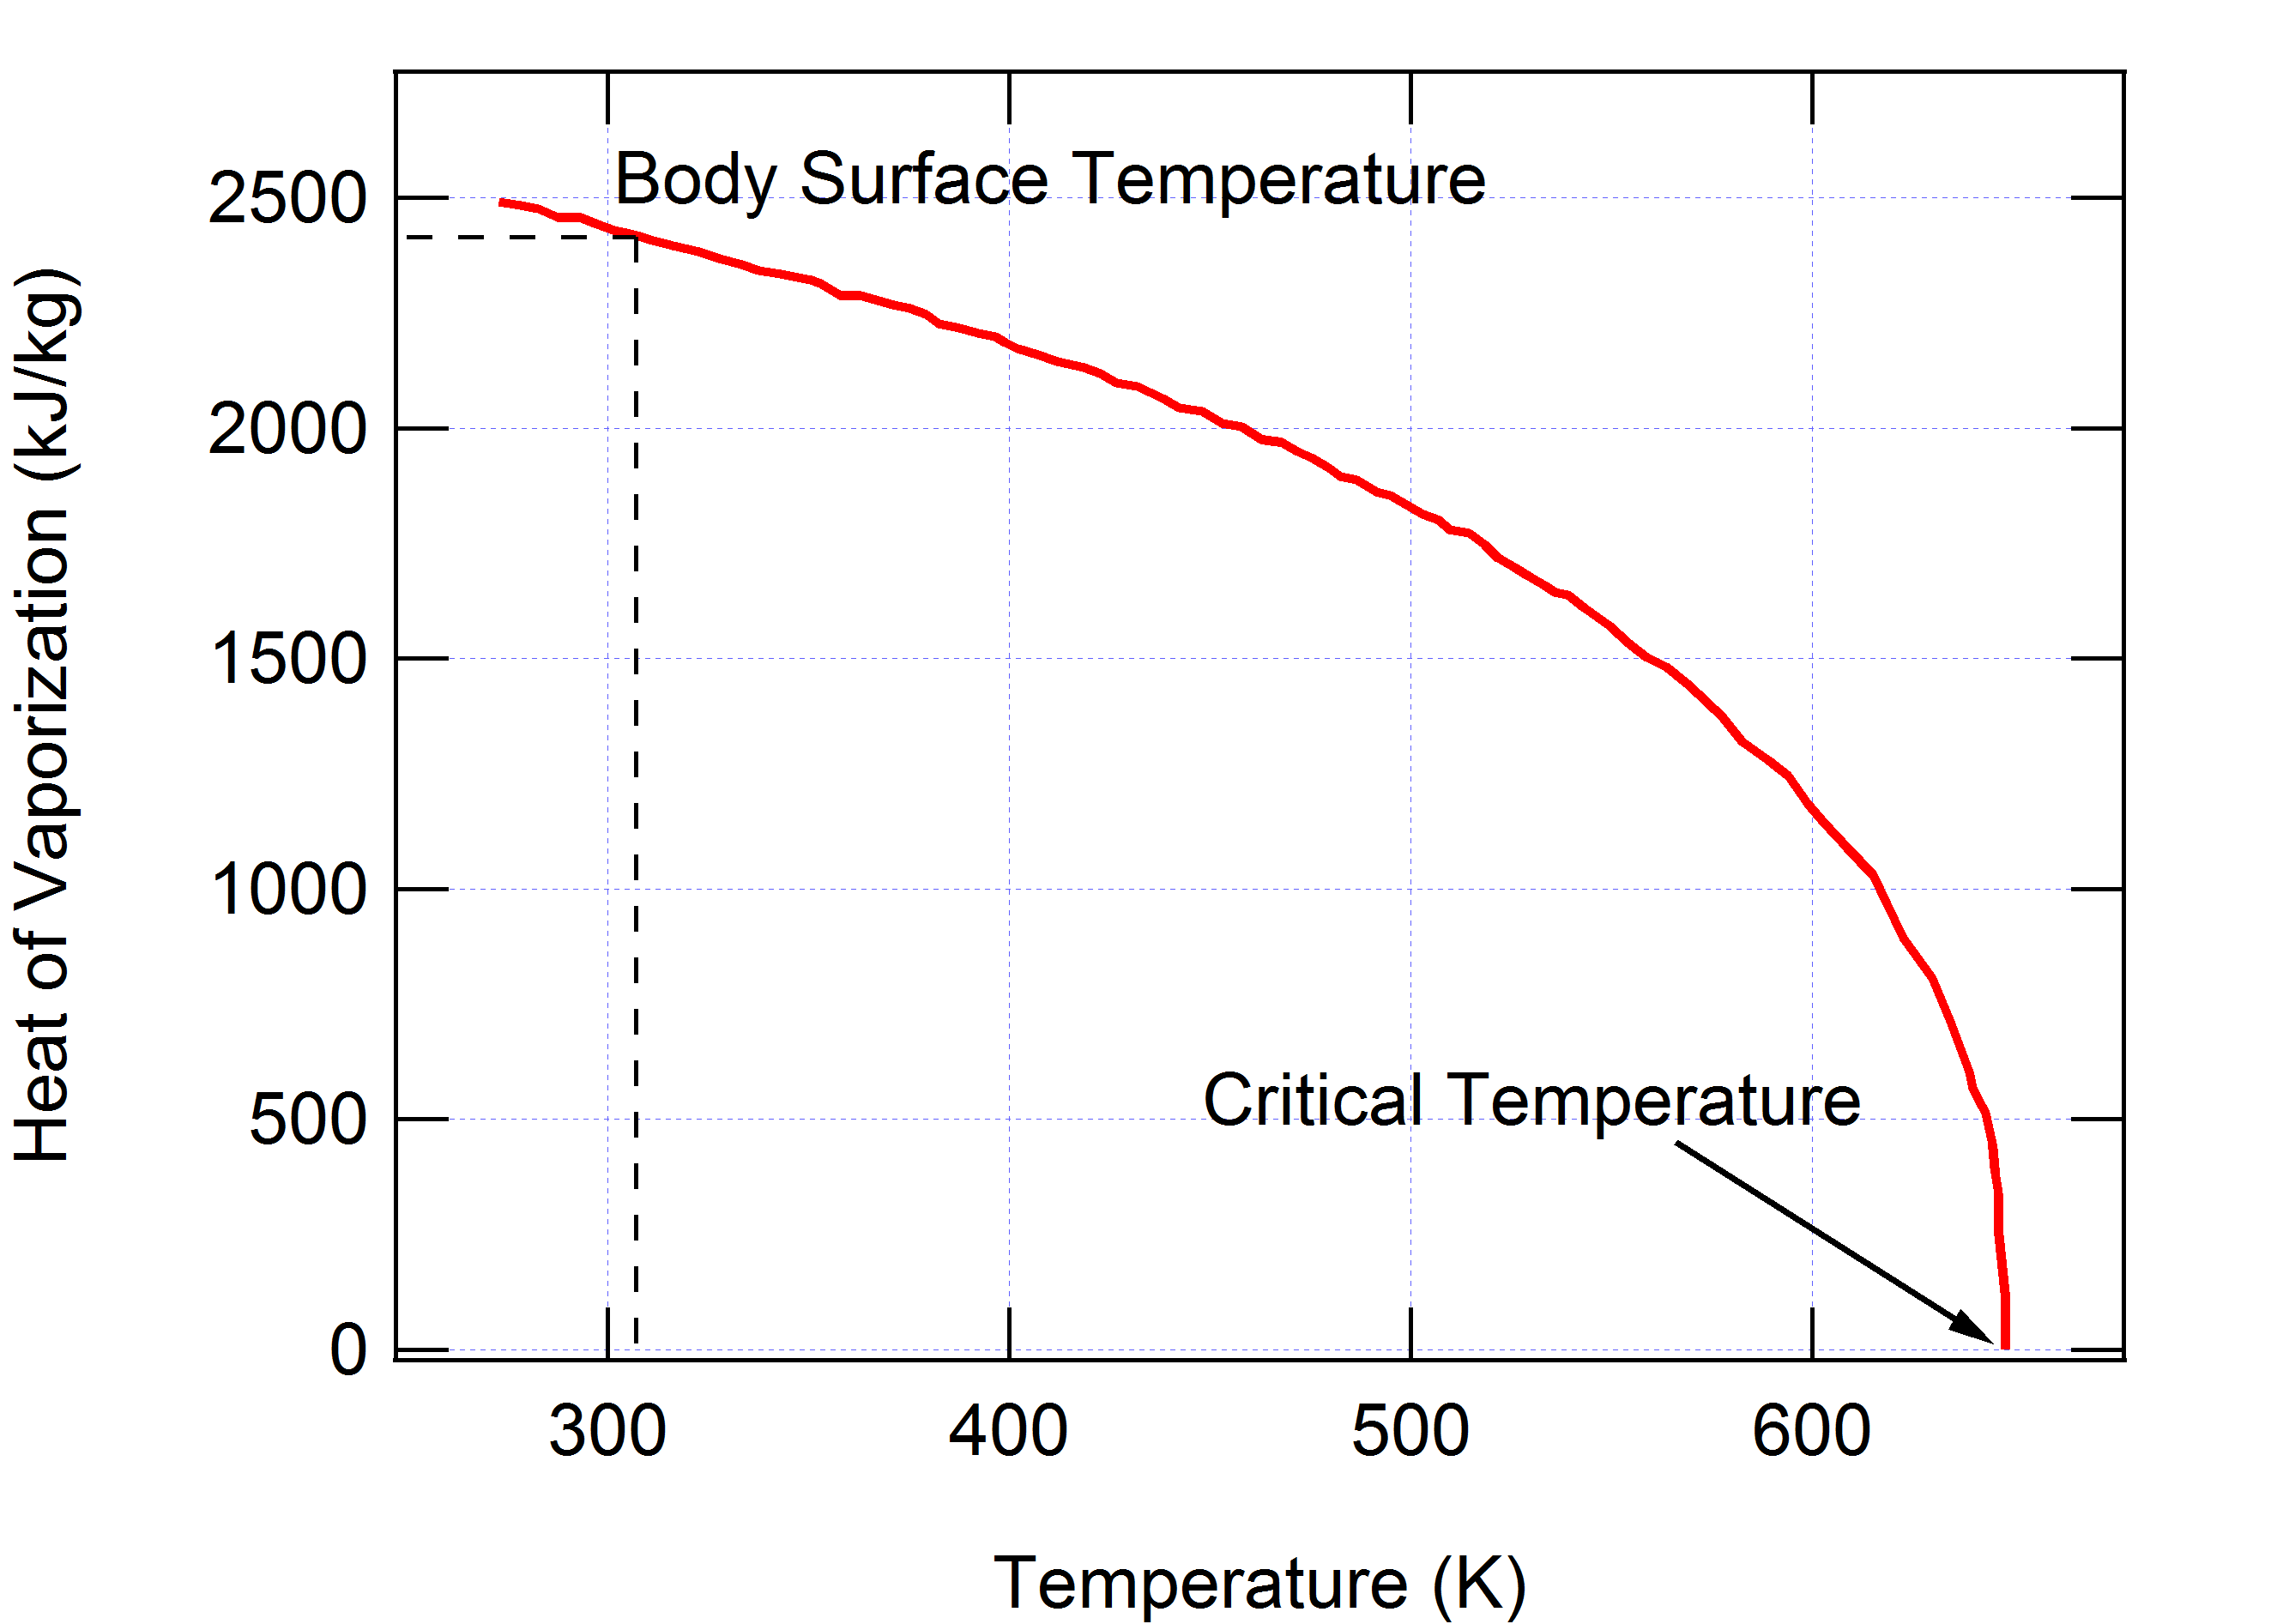
\includegraphics[width=\textwidth]{./figures/Topic4/Fig4-2.png}
	\caption{The heat required to evaporate water at temperatures ranging from freezing to the critical point above which only the gaseous phase of water exists.}
	\label{Fig4-2}
\end{figure}
Without sweating, the average person loses about 0.6 liters of water per day due to evaporation, equivalent to a cooling rate of 15 kcal/hour, or 18 W.  Under extreme conditions and for acclimatized persons, a body can lose as much as two liters of water per hour.  At this rate, the person will cool at a rate of 1,160 kcal per hour, equivalent to 1300 W, by sweating alone!

\subsection{Conduction}

Conduction refers to heat transfer within a body or between two bodies in contact.  Heat always moves from areas of high temperature towards areas of low temperatures.  Typically, the human body is warmer than its environment, so heat moves from the body to surrounding air or to objects in contact with our skin.  The power dissipated from our skin to the environment is governed by the equation
\begin{equation}\label{eqn4-3}
P_{conduction} = \frac{kA\left(T-T_{ambient}\right)}{d}
\end{equation}
where $k$ is the conductivity of air ($k$ = 0.024 W/m$\cdot$K) and $d$ represents the thickness of the insulating layer or air that surrounds the body ($d\approx$ 1 cm with clothes and 0.3 cm without).  Using the $d$ value for clothing and the values used previously for $A$, $T$, and $T_{ambient}$, the heat loss due to conduction is about 33 W.

\section{Regulation of Body Temperature}

As stated before, body temperature is regulated by an area of the brain called the hypothalamus.  Heat sensors in the skin and throughout the body respond to temperature changes by stimulating the hypothalamus to evoke certain responses.  These responses are described below.    

\subsection{Responses to High Temperatures}

\subsubsection{Vasodilation}
Along with nutrients, blood carries heat.  Blood circulating deep within the body picks up heat, which can be subsequently carried by the circulation to the skin.  There the heat is dissipated into the environment and the cooled blood re-enters the body ready to transfer more heat.  Our bodies possess a heat sensing mechanism that regulates blood flow to the skin in relation to the need for heat dissipation. The blood flow is regulated by a network of blood vessels underneath the skin that contract or dilate as needed. For instance, these blood vessels dilate as the body’s temperature rises above the optimal range to divert greater blood flow to the skin. As much as one-third of the cardiac output can be rerouted so that heat can be removed from the body.  The effectiveness of this mechanism is demonstrated in Fig.~\ref{Fig4-3}, which shows how much heat conduction from the core to the skin takes place as the ambient temperature rises.  
\begin{figure}[h]
	\centering
	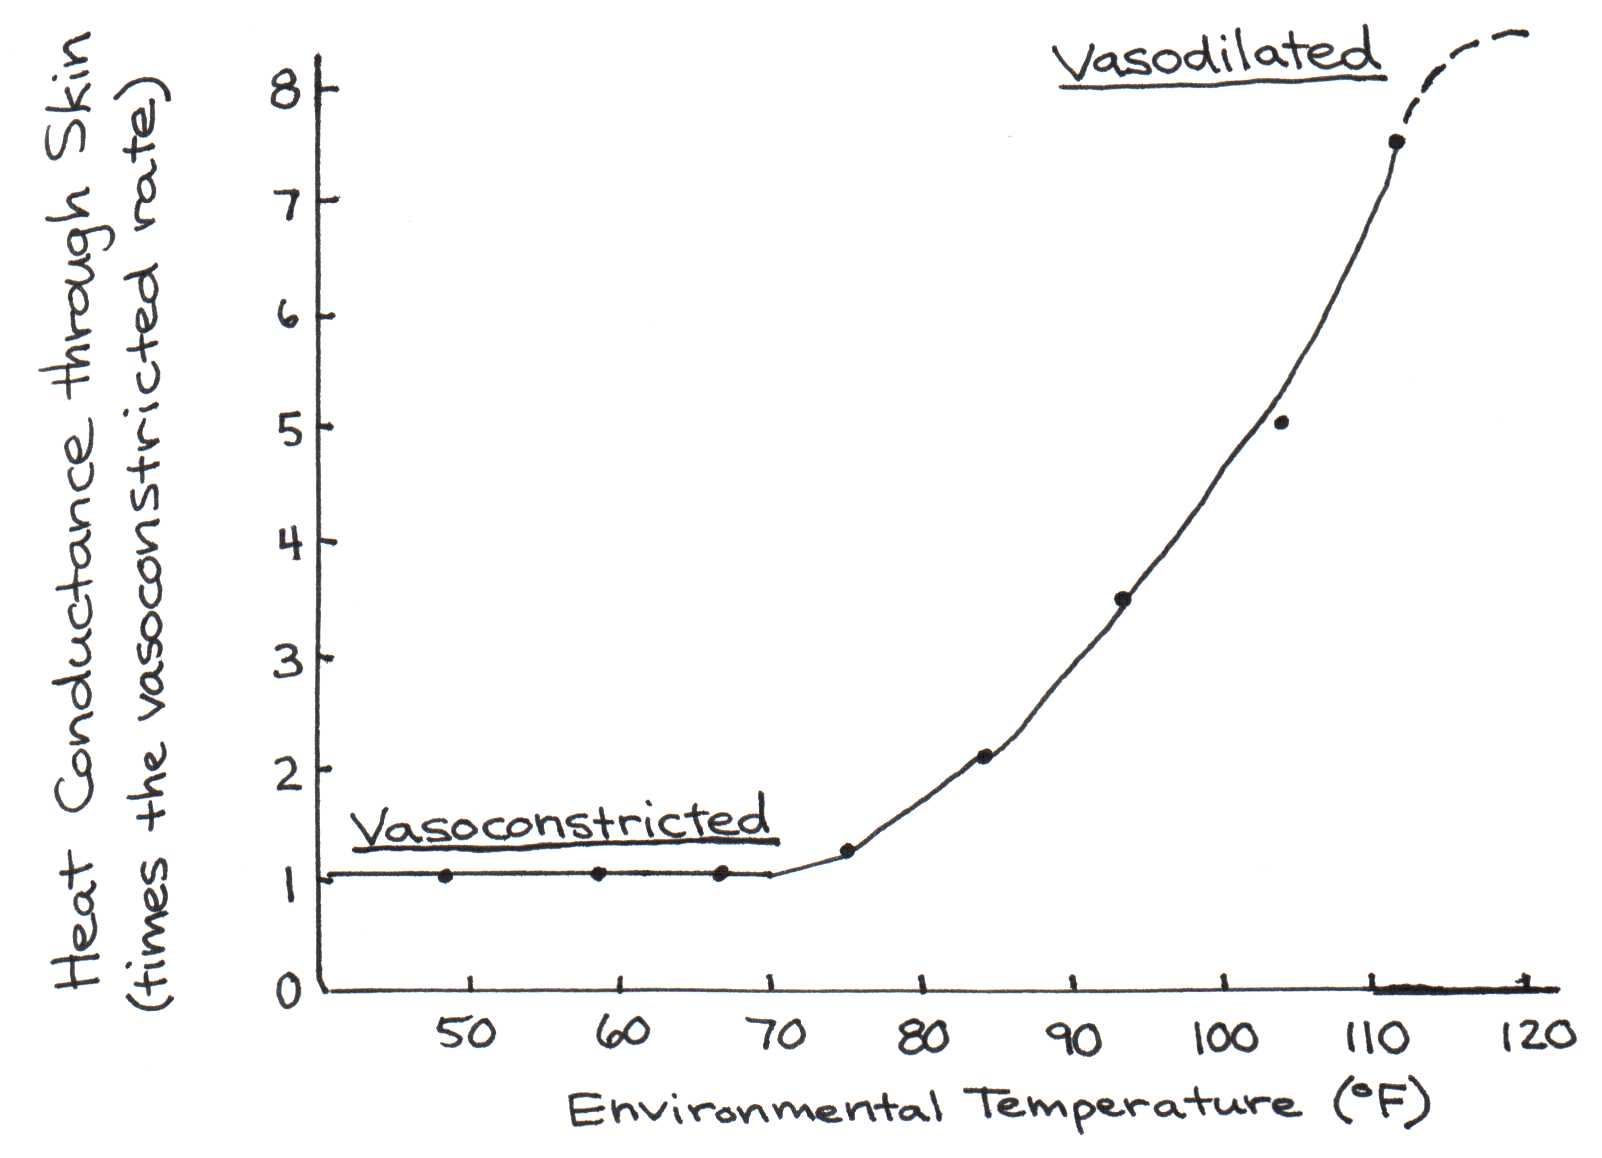
\includegraphics[width=\textwidth]{./figures/Topic4/Fig4-3.jpg}
	\caption{Effect of ambient temperature changes on heat conductance from the body core to the skin surface.  At 110$^{\circ}$F, the skin loses seven times as much heat through the skin because of vasodilation.}
	\label{Fig4-3}
\end{figure}
  
\subsubsection{Sweating and Behavioral Cooling}

As already discussed, sweating is the predominant form of evaporative cooling.  Many animals that do not sweat, like dogs and birds, pant to increase evaporative cooling in their mouths and throats.  Since a wet body surface can be 50--100 times more effective at conducting heat than a dry one, most animals also find relief from the hot sun by bathing in cold water.  A cold beverage on a warm day really does cool you down-heat from your core is transmitted to the liquid, making you less hot.

\subsubsection{Reduction of Metabolism}

A third way to reduce heat is to reduce the amount of metabolic activity going on inside the body.  The hypothalamus sends signals to other parts of the brain that control chemical pathways, telling them to slow down.  

\subsection{Responses to Low Temperatures}

\subsubsection{Vasoconstriction}

Vasoconstriction on the skin is exactly the opposite of vasodilation—heat is retained in the core by limiting the blood flow near cooler regions, like the skin.  Many marine animals and endotherms have adapted a counter-current heat exchanger, a unique arrangement of blood vessels that allows heat to pass from the warmer blood in the arteries to the cooler blood in the veins, minimizing heat loss outside of the body.  

\subsubsection{Piloerection}

Recall from Eq.~\ref{eqn4-2} the inverse relation between $d$, the thickness of air insulating the body, and the power dissipated by the body.  Many animals can trap more insulating air around the skin by fluffing up fur or feathers.  This method of decreasing heat loss is called piloerection.  Goose bumps are an evolutionary throwback to a time when our more hairy ancestors made use of this ability.

\subsubsection{Increased Heat Production}

Shivering, the increased contraction of muscles, produces heat in the body.  Alternatively,  hormones can trigger cellular metabolism to produce heat instead of ATP.  This is called nonshivering thermogenesis.  Both of these processes actually produce more heat rather than simply preventing heat from escaping the body.    

 %Thermoregulation
\setcounter{chapter}{5}
\setcounter{section}{0}
\setcounter{figure}{0}
\setcounter{equation}{0}
\setcounter{table}{0}
\chapter*{
\includegraphics[width=\textwidth]{./figures/Topic5/Topic5.jpg}}
\addcontentsline{toc}{chapter}{Topic 5: Optics in Vision and Eyesight Correction}

\section{Introduction}

The eye is able to detect light over a range of brightness of ten billion to one. It can bring into focus both starlight from millions of light-years away and light reflected from this page, about 20 cm away.  The shape and optical properties of the eye allow light entering the iris to form an image on the back surface of the eye called the retina.  Two types of photoreceptive cells on the retina, the rods and the cones, are responsible for interpreting brightness and color.  

We will first review the principles of optics and apply them to the eye.  Then we will discuss vision problems associated with small aberrations in the shape of the eye and how corrective eyewear and surgery can improve vision.

\section{Geometrical Optics: A Review}

\subsection{Properties of Light}
In a vacuum, all electromagnetic waves, including visible light, travel at a singular speed ($3.0\times10^8$ m/s).  The speed of light in air is approximately the same, but in water and other dense transparent media, it travels significantly slower.  The index of refraction, denoted by $n$, is the ratio of the speed of light c in vacuum to the speed of light $v$ in the material:
\begin{equation}\label{eqn5-1}
n = \frac{c}{v}
\end{equation}
Note that the larger the value of $n$, the slower the speed of light in the medium. The value of $n$ is always greater than 1 because light is limited to its vacuum speed. We will approximate the index of refraction in air to 1 and in water to 1.33.

The speed of light waves in a medium $v$ is related to frequency $f$ and wavelength $\lambda$ according to the well-known equation 
\begin{equation}\label{eqn5-2}
v = \lambda f
\end{equation}
As light passes from one medium to another, frequency remains constant.  Consequently, according to Eq.~\ref{Fig5-2}, the wavelength must decrease as the speed v decreases and vice-versa.  Fig.~\ref{Fig5-1} illustrates this effect as light waves pass from air into glass.  
\begin{figure}[h]
	\centering
	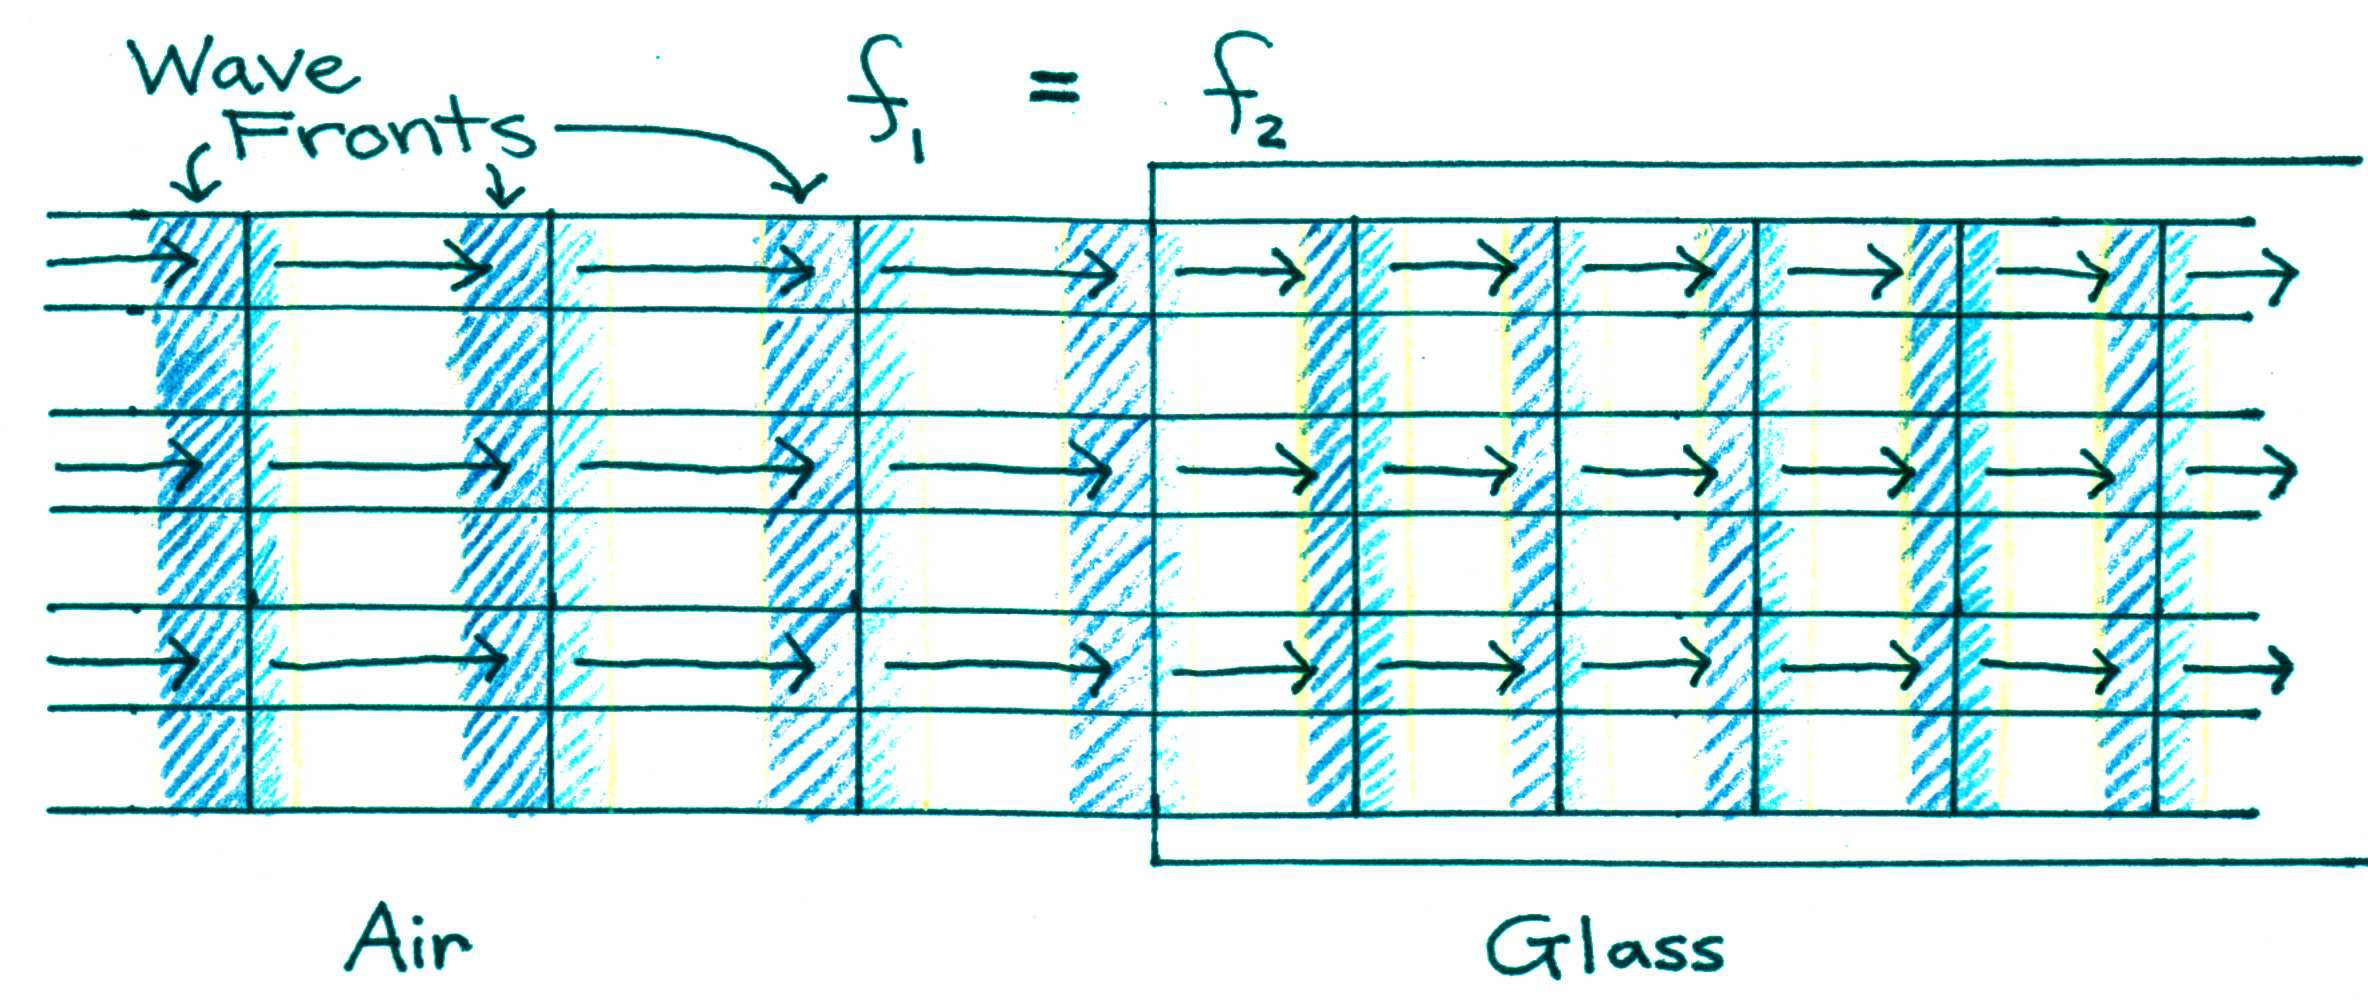
\includegraphics[width=4.0in]{./figures/Topic5/Fig5-1.jpg}
	\caption{Effect of light passing from a less dense medium (air) to a more dense medium (glass).  The wave slows down and the wavelength decreases.}
	\label{Fig5-1}
\end{figure}
When light strikes the surface of a transparent medium at an angle other than normal incidence, it is bent at the boundary (see Fig.~\ref{Fig5-2}). This bending of light due to a change in wave speed is called refraction. Effect of light passing from a less dense medium (air) to a more dense medium (glass).  The wave slows down and the wavelength decreases.
\begin{figure}[h]
	\centering
	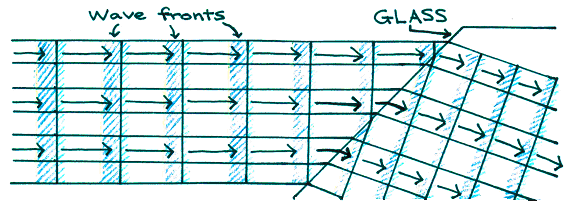
\includegraphics[width=4.0in]{./figures/Topic5/Fig5-2.png}
	\caption{Refraction at the interface of air and glass.   Note that the wavelength still shortens to compensate for decreased wave speed.}
	\label{Fig5-2}
\end{figure}
The ability to bend light can be exploited to focus light using the effect illustrated in Fig. 2. For instance, some focusing can be achieved with the crude lens design shown in Fig.~\ref{Fig5-3}, although not very effectively since not all portions of the incoming wave converge to a single point. A better design is achieved with a spherical surface, which is the shape that most is lenses utilize. 
\begin{figure}[h]
	\centering
	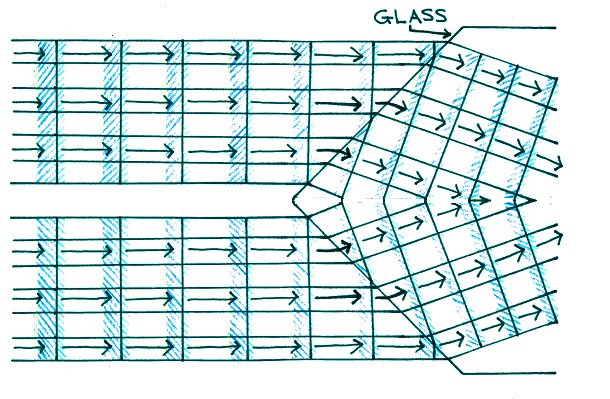
\includegraphics[width=4.0in]{./figures/Topic5/Fig5-3.png}
	\caption{Crude lensing effect created by a piece of glass with a triangular profile.}
	\label{Fig5-3}
\end{figure}

As we shall see, different parts of the eye have different indices of refraction and spherical shapes. Together they form a system capable of focusing light from near or distant objects and still produce a clear image on the retina.

\subsection{Thin Lenses} 

The focal point of a lens is defined as the point at which parallel incoming rays (like from a distant light source or a laser) converge. For thin lenses, focal length f is the distance from the focal point and the center of the lens.  
There are two main types of thin lenses: converging (positive) lenses and diverging (negative) lenses.  Converging lenses, also called focusing lenses, are thicker at their center than at their edges and have a positive focal length; diverging lenses are thicker at their edges than at their centers and have a negative focal length.  Figure \ref{Fig5-4} shows that parallel rays entering a converging lens from the left converge at the focal point on the outgoing (right) side of the lens.   Also shown in Figure \ref{Fig5-4} are parallel light rays entering a diverging lens.  If we were to extend the diverging rays back to the left, they would appear to intersect (converge) at the focal point on the incoming side of the lens.  As this focal point is on the side opposite to the outgoing light, the focal length is negative.  
\begin{figure}[h]
	\centering
	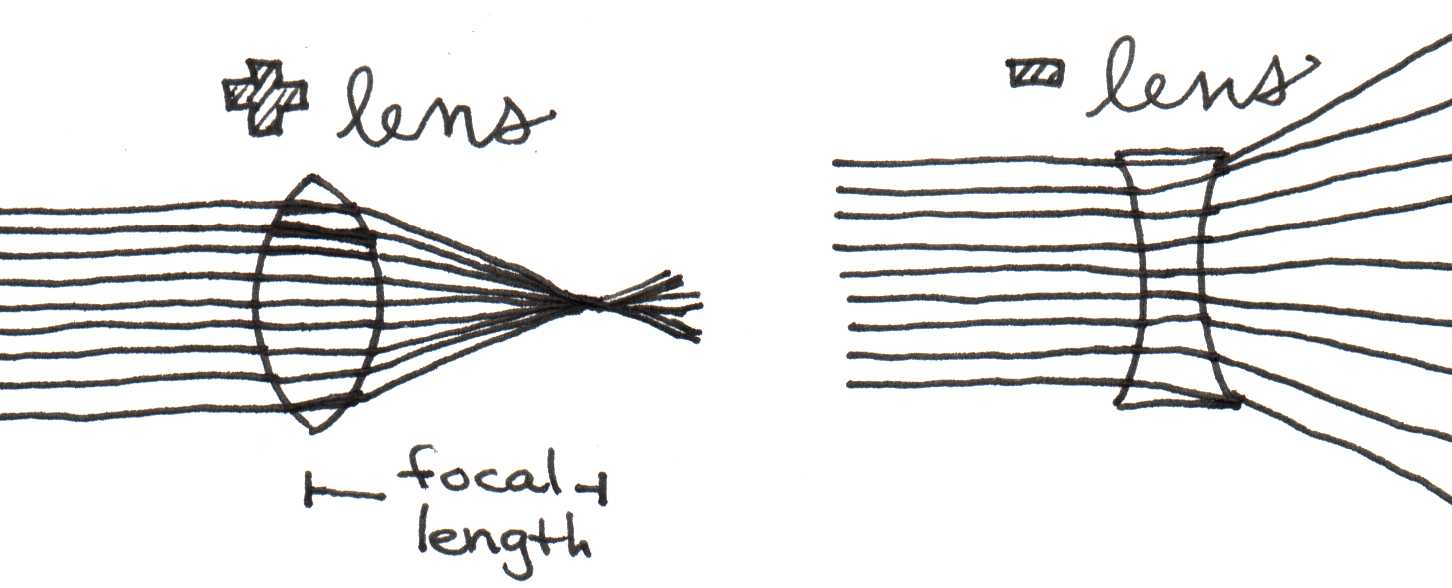
\includegraphics[width=4.0in]{./figures/Topic5/Fig5-4.jpg}
	\caption{Left: light rays entering a converging (positive) lens.  Right: light rays entering a diverging (negative) lens.}
	\label{Fig5-4}
\end{figure}

As the distant source moves closer, as shown in Fig.~\ref{Fig5-5}a and Fig.~\ref{Fig5-5}b, the focal point moves farther away from the lens. If $s$ is the distance from the object (light source) to the lens and $s'$ is the distance from the lens to the image (focus), $s$ and $s'$ are related to $f$ by the thin lens equation.
\begin{equation}\label{eqn5-3}
\frac{1}{f} = \frac{1}{s} + \frac{1}{s'}
\end{equation}
Fig.~\ref{Fig5-5}a and Fig.~\ref{Fig5-5}b also illustrate a crucial point about the ability of a lens to focus light from objects at varying distances. Suppose our eyesight is focused on a distant object to such that it produces a sharp image on the retina, located at the focal point of Fig.~\ref{Fig5-5}a. Now consider what would happen if the object moved closer and the image distance shifts as shown in Fig.~\ref{Fig5-5}b. The image should no longer be in focus on the retina, implying that the image should look fuzzy now. The only way to overcome this problem, that is, to keep the image in the same location, would be to decrease the focal length of the lens by making it more spherical as suggested in Fig.~\ref{Fig5-5}c. 
\begin{figure}[htb]
	\centering
	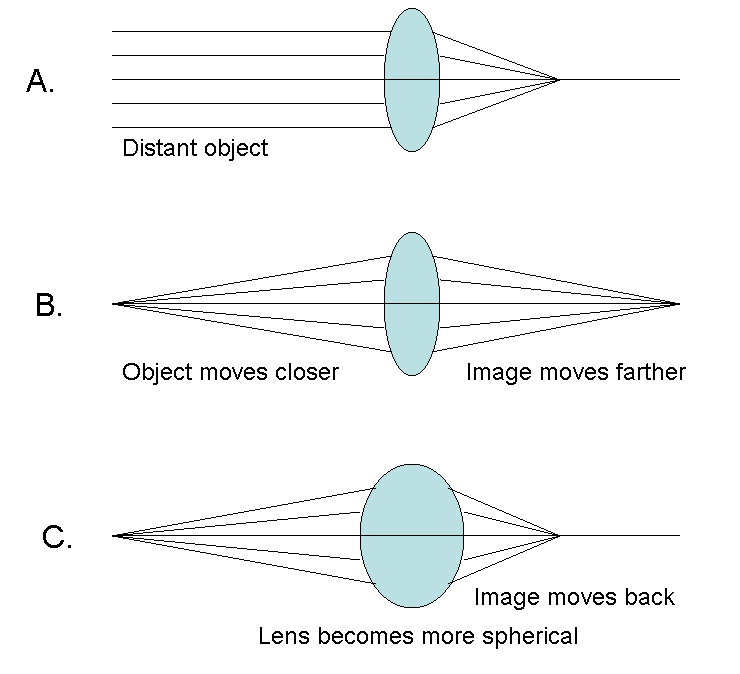
\includegraphics[width=4.0in]{./figures/Topic5/Fig5-5.png}
	\caption{Effects of image distance and lens shape on the location of the image distance.}
	\label{Fig5-5}
\end{figure}
As we shall see shortly, our eyesight possesses a mechanism that alters its focal length as needed to accommodate different objects distances.

\subsection{Refractive Power}

The strength of convergence of a lens depends on its refractive power, which is defined as the reciprocal of the focal length $f$ given in meters:
\begin{equation}\label{eqn5-4}
P = \frac{1}{f}
\end{equation}
The unit of power is the diopter, where 1 diopter = 1 m-1.  Figure 6 compares the power of three different lenses. 
\begin{figure}[htb]
	\centering
	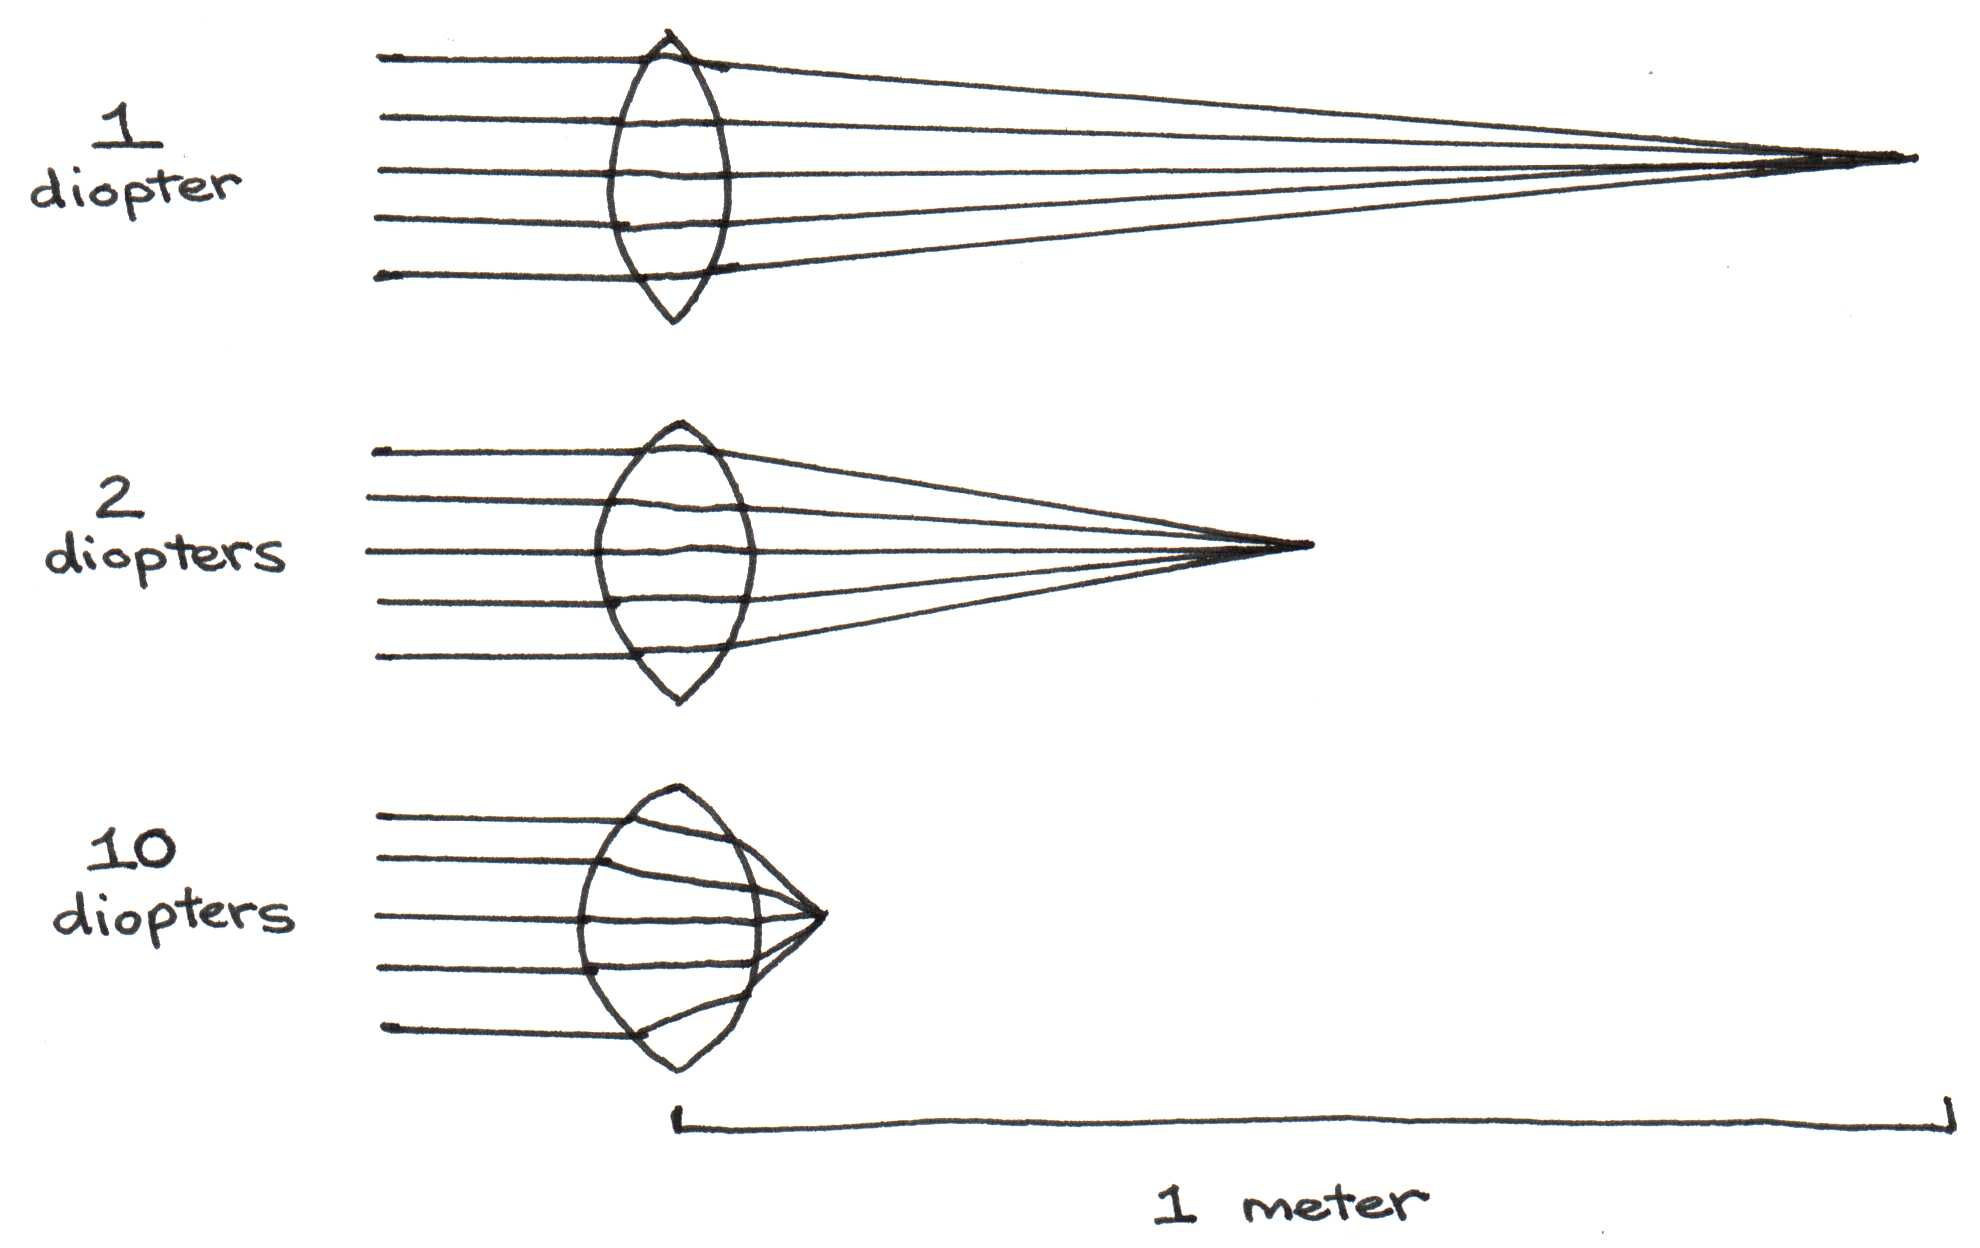
\includegraphics[width=4.0in]{./figures/Topic5/Fig5-6.jpg}
	\caption{The power of a lens with focal length $f$ = 1 m is $P$ = 1 diopter; $f$ = 0.5 m, $P$ = 2 diopters; $f$ = 0.1 m, $P$ = 10 diopters.}
	\label{Fig5-6}
\end{figure}
When two or more lenses are combined, the resulting refractive power is equal to the sum of the refractive powers of each lens.
\begin{equation}\label{eqn5-5}
P_{total} = \frac{1}{f_{lens1}}+\frac{1}{f_{lens2}}+\frac{1}{f_{lens3}}+\cdots
\end{equation}
Refractive power depends not only on the curvature of both surfaces of the lens, but also on the indices of refraction of the lens and the outside medium.  
\begin{equation}\label{eqn5-6}
P = \frac{1}{f} = \left(n_{lens}-n_{medium}\right)\left(\frac{1}{R_1}-\frac{1}{R_2}\right)
\end{equation}
where $R_1$ is the radius of curvature of the first surface light encounters as it passes through the lens, while $R_2$ is the radius of curvature of the exiting surface.  When the center of curvature points in the direction of light, as is the case for $R_1$ in Fig.~\ref{Fig5-7}, its value is positive. Conversely, when the center of curvature points in the direction opposite to that of light, as is the case for $R_2$ in Fig.~\ref{Fig5-7}, its value is negative. Equation (6) is called the lensmaker's equation.
\begin{figure}[h]
	\centering
	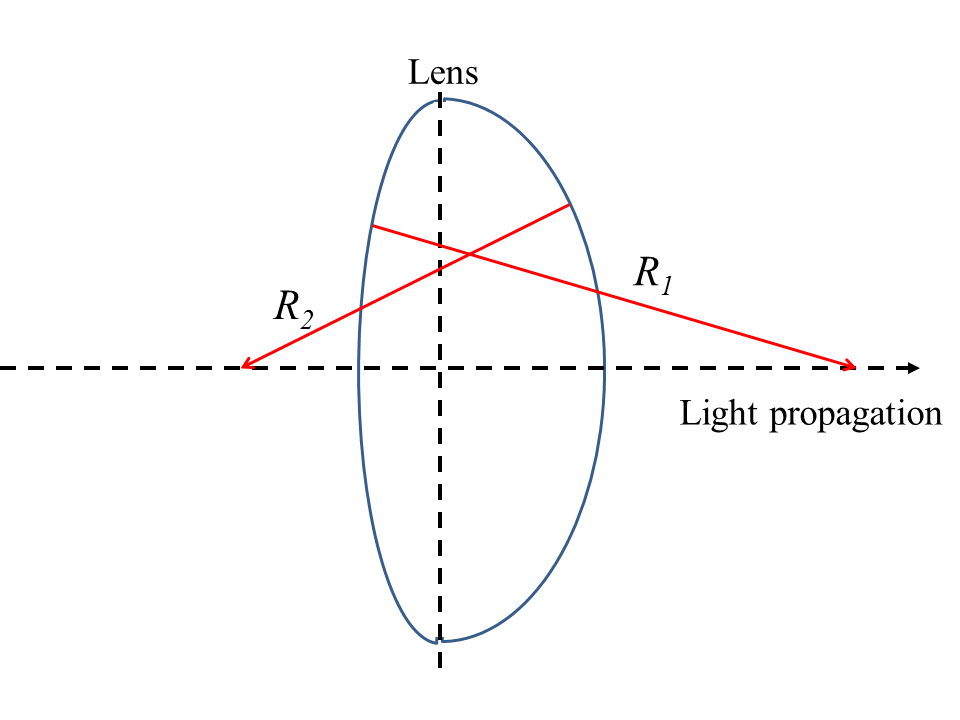
\includegraphics[width=3.5in]{./figures/Topic5/Fig5-7.png}
	\caption{Diagram of a lens for using the lensmaker's equation (Eqn.~(6)).}
	\label{Fig5-7}
\end{figure} 

\section{Optics of the Eye and Vision}

With this background in optics, we are now ready to examine the optical components of the eye.  Figure \ref{Fig5-8} gives the indices of refraction for the optical materials through which light must pass.
\begin{figure}[h]
	\centering
	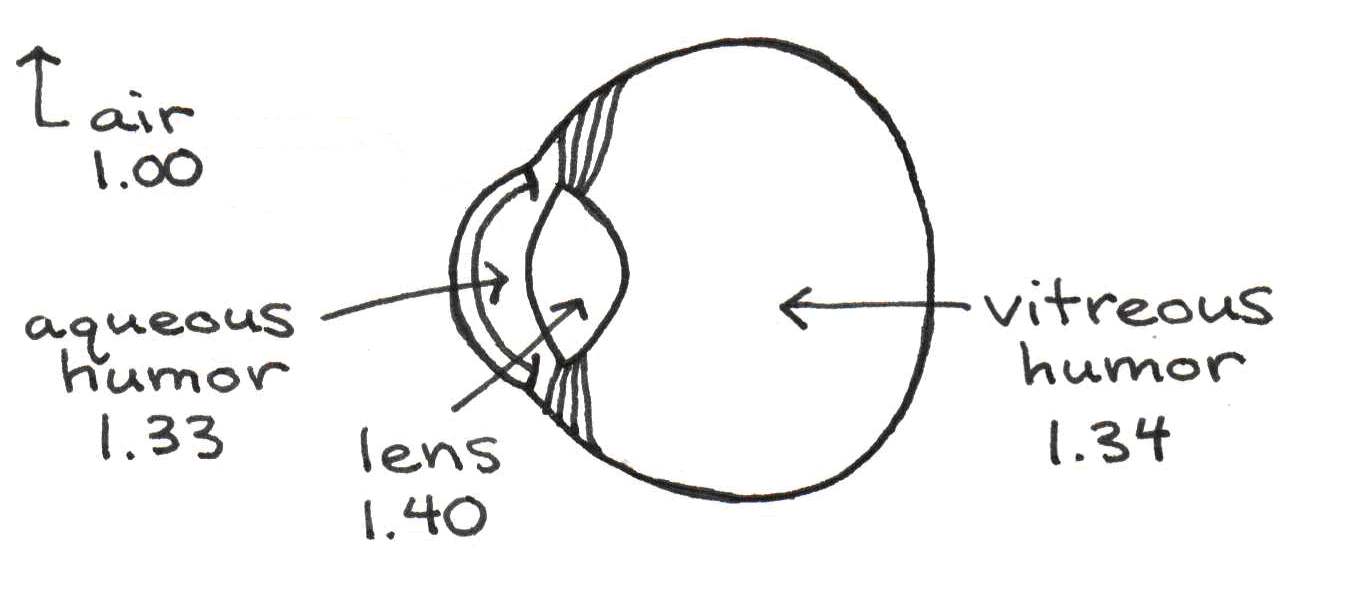
\includegraphics[width=3.5in]{./figures/Topic5/Fig5-8.png}
	\caption{Optical components of the eye and their indices of refraction.}
	\label{Fig5-8}
\end{figure}
The components of the eye are as follows:
\begin{itemize}
\item Cornea.  The cornea is an optically clear membrane that holds in place the fluids inside the eye.  It is roughly spherical in shape.
\item Pupil.  The pupil is the aperture through which light passes.  Its diameter can vary from 1.5 mm to 8.0 mm, controlling the amount of light reaching the back of the eye by a factor of about 30.  As we will see, the diameter of the pupil has a significant impact on the perceived field depth and clarity of an object.
\item Iris.  The iris is the colored muscle surrounding the pupil.  When it contracts, the pupil dilates (becomes bigger), allowing more light to enter the eye.  When it relaxes, the pupil constricts.  The iris is often compared to the diaphragm of a camera.
\item Aqueous humor and vitreous humor.  The aqueous and vitreous humors are the fluids that keep the eye inflated.  The aqueous humor, between the cornea and the lens, consists mainly of water.
\item Crystalline lens.  The lens is composed of a strong elastic membrane that encapsulates a viscous, protein-rich substance.  Its spherical shape is controlled by a muscle.  When the muscle contracts, the lens thickens, increasing the refractive power of the lens.  This is what allows us to see objects up close.  When the ciliary muscle relaxes, the lens flattens, making distance vision possible.
\item Retina.  The retina is the layer of tissue lining the back of the eye.  It is covered with two types of light receptors called rods and cones.  These receptors convert light into nerve impulses that travel to the visual cortex where they are interpreted.
\end{itemize}
 
\subsection{Refractive Power of the Eye}

The lens and the cornea are the components of the eye most responsible for refraction.  We will now find the refractive power of each component separately and then find the total refractive power of the eye by summing these values.
The refractive power of the eye is due mostly to refraction from air to the aqueous humor, which is dictated by the shape of the cornea.  It can be calculated using Eq.~\ref{Fig5-6}.  Since the cornea only has one surface, $R_1$ is simply the radius of curvature of this surface ($\sim$ 8 mm. FYI this is one of the numbers characterizing contact lenses so that they fit properly.), and $R_2$ is infinity.  Approximating the index of refraction of the aqueous humor is 1.33, we see that 
$$P = \left(1.33 - 1.00\right)\left(\frac{1}{0.008}-\frac{1}{\infty}\right) = 41.25~{\rm diopters}.$$
We also use Eq.~\ref{Fig5-6} to calculate the refractive power of the lens.  The radii of curvature $R_1$ and $R_2$ for the lens in the eye are 0.0102 and -0.0060 m respectively, when the eye focuses on distant objects. The index of refraction of the lens is equal to 1.40, while that of the surrounding medium is 1.33 and 1.34 on either side. For simplicity we will average these two values and set the average index of refraction of the lens to be 1.335. Thus,  
$$P = \left(1.40 - 1.335\right)\left(\frac{1}{0.0102}+\frac{1}{0.006}\right) = 17.20~{\rm diopters}.$$
Thus, by Eq.~\ref{Fig5-5}, the total refractive power of the eye is about 58 diopters.  Note that this value was calculated for an eye focusing on distant objects.

\subsection{Accomodation}
To focus clearly on nearby objects, the eye must increase its total refractive power.  As mentioned earlier, it accomplishes this by changing the shape of the lens, a process called accommodation.  Figure \ref{Fig5-9} illustrates how accommodation occurs.
\begin{figure}[h]
	\centering
	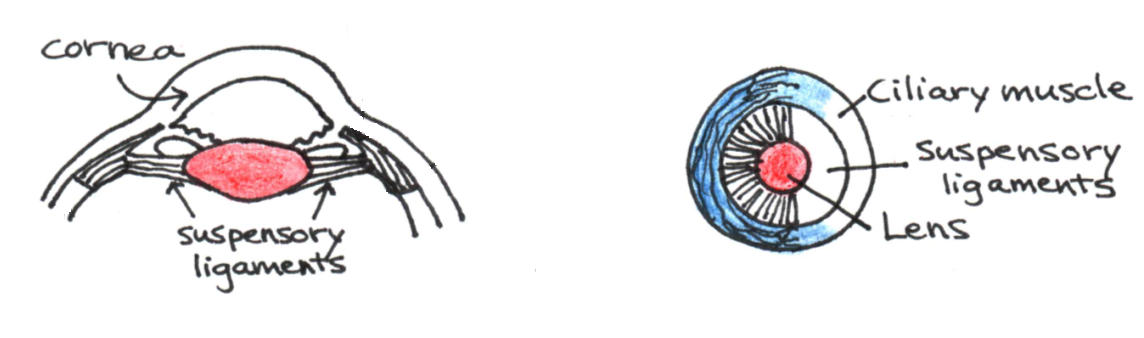
\includegraphics[width=\textwidth]{./figures/Topic5/Fig5-9.png}
	\caption{Mechanism of accommodation.}
	\label{Fig5-9}
\end{figure}  
The ciliary muscle is attached to the suspensory ligaments, which hold the lens in place.  When the ciliary muscle relaxes and expands, it pulls the ligaments away from the lens. The resulting increased tension on the lens causes it to assume the flattened shape needed for distance vision.  When the ciliary muscle contracts, the ligaments are forced inwards, causing the lens to assume a more spherical shape in which the radii of curvature increase.  This allows the eye to focus on nearby objects.  Through accommodation, the refractive power of the lens can increase from 17 diopters up to 31 diopters, a 14 diopter increase from normal refractive power.  Thus, it is said that the lens has an accommodation power of 14 diopters.
 
As we age, the lens slowly grows and loses its elasticity.  When this occurs, the ciliary muscle cannot cause it to assume a spherical shape as easily, and accommodation power diminishes.  Table \ref{table5-1} shows the average accommodation power for several age groups.
\begin{table}[h]
\begin{center}
\begin{tabular}{|l|c|}
\hline
Age & Accomodation Power (diopters) \\
\hline
Children & 14 \\
18--22 & 11--12 \\
45--50 & 2--4 \\
60--70 & 0--1\\
\hline
\end{tabular}
\caption{Accommodation power diminishes with age.}
\label{table5-1}
\end{center}
\end{table}
This phenomenon is inevitable -— it is the reason people begin to wear reading glasses when they reach middle age.

\subsection{Visual Acuity}

Visual acuity is defined as ability to visually resolve fine detail. The most common measure of acuity is the Snellen chart, such as the one shown in Fig.~\ref{Fig5-10}, which identifies what a person can see at 20 feet relative to what person with normal eyesight can see x feet way. Thus, 20/20 is normal, whereas 20/200 is regarded as very poor eyesight. Contacts, eyeglass, and surgery can improve many of the eye’s refractive errors that cause poor visual acuity. In some cases however, the best eyesight correction that can be afforded is 20/200, at which point one is classified as legally blind.
\begin{wrapfigure}{l}{0.5\textwidth} 
\vspace{-20pt}
  \begin{center}
    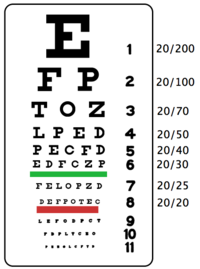
\includegraphics[width=0.4\textwidth]{./figures/Topic5/Fig5-10.png}
    \caption{A typical Snellen chart used by optometrist to determine visual acuity.}
    \label{Fig5-10}
  \end{center}
  \vspace{0.25in}
\end{wrapfigure}

In order to see the letters on the chart corresponding to 20/20, an eye must have the ability to revolve points separated by as little as an arc minute (= 1/60 of a degree or $2.9\times10^{-4}$ radians. To put it into perspective, consider two small light sources separated by a distance x = 1 cm, as shown in Fig.~\ref{Fig5-11}. As you step back from those two sources by a distance l, the angle $\theta$ decreases and eventually reaches the limit of visual resolution, i.e.,  $\theta = 2.9\times10^{-4}$ radians. At this point, the corresponding distance $L$ is related to the angle $\theta = 2.9\times10^{-4}$ radians and $x$ by $\tan(2.9\times10^{-4}$ radians) = 1cm/$L$, from which we obtain a distance $L$ of 34 meters (100 ft). 

\begin{figure}[b]
	\centering
	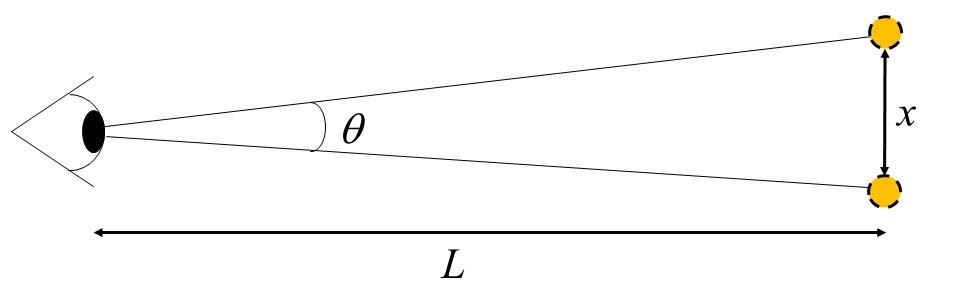
\includegraphics[width=4.0in]{./figures/Topic5/Fig5-11.jpg}
	\caption{Diagram demonstrating the relevant variables for resolving two objects spaced a distance $x$ apart and a distance $L$ away from the viewer.}
	\label{Fig5-11}
\end{figure}

As we shall see now, the above limit of visual acuity is largely due to the wave nature of light. Before we discuss this interesting feature we must first consider how far apart those two luminous objects are when imaged on the retina. To calculate this distance we can make use of the relation between object and image sizes introduced in your Introductory Physics class
$$\frac{\rm Image~Height}{\rm Object~Height} = \frac{\rm Image~Distance}{\rm Object~Distance}$$
or
$$\frac{\rm Image~Height}{x}=\frac{\rm Image~Distance}{L}$$
Here the image distance corresponds to the distance between the cornea and the retina, which is roughly 1.7 cm. Therefore,
$$\frac{\rm Image~Height}{1~{\rm cm}}=\frac{1.7~{\rm cm}}{3400~{\rm cm}}$$
From the above equation one can work out that the separation between the imaged light sources on the retina (the image height) is about 5 $\rm \mu$m.  The question then is how this distance is related to the diffraction limit.

Diffraction, as you may recall, is the phenomenon that describes how waves spread out as they propagate.  Fig.~\ref{Fig5-12} below shows a diffraction pattern from light entering a small aperture.  Plane waves entering the aperture from the left appear collimated at first, but rapidly evolve into a cone of diverging waves.
\begin{figure}[h]
	\centering
	\includegraphics[width=4.0in]{./figures/Topic5/Fig5-12.png}
	\caption{Diffraction produced as a wave passes through an aperture.}
	\label{Fig5-12}
\end{figure}
If $\theta$ is half the angle of divergence, $D$ is the size of the aperture, and $\lambda$ is the wavelength of light, diffraction theory predicts that these quantities are related by the formula
\begin{equation}\label{eqn5-7}
D = \frac{1.22\lambda}{\theta}
\end{equation}
One of the beautiful things about the laws of physics is that they are time reversible. That is, if you were to reverse the time evolution of diffraction the same way you would reverse the footage in a movie, the backwards movement still obeys the laws of physics. We can extend this simple principle to our present situation and conclude that when waves are focused into a cone of half angle $\theta$ they will focus to a spot with a size $D$. The size of the spot $D$ is dictated by the half-angle of convergence $\theta$ and the wavelength $\lambda$ dictate according to Eq.~\ref{Fig5-7}.

The implication for the eye is illustrated with Fig. 13. The optics in the eye produces a converging wave with a half angle that is dictated by the size of the pupil. 
\begin{figure}[h]
	\centering
	\includegraphics[width=4.0in]{./figures/Topic5/Fig5-13.png}
	\caption{The point of focus on the retina is finitely sharp due to diffraction.}
	\label{Fig5-13}
\end{figure}  
Let $q$ be the diameter of the pupil (in bright light, $q$ = 1.5 mm), $l$ be the distance from the pupil to the retina (1.5 cm), and $\theta$ be half the angle formed by the cone of light entering the eye.  Since $\tan\theta=q/2l$, and by the small angle approximation $\tan\theta\approx\theta$, we see that $\theta\approx0.05$ radians.  If we assume that the incoming light has wavelength 500 nm, the smallest point of light on the retina is found by solving for $D$:
$$D = \frac{1.22\lambda}{\theta}=\frac{1.22\cdot 5\times10^{-7}}{0.05}.$$
So let us see how this spot size relates to our earlier calculation of the separation between the retinal images of two light sources at the limit of visual acuity. The spot size appears to be a factor of two larger than the estimated separation of 5 um, and for a good reason. When two spots are separated by a full spot size as depicted in Fig.~\ref{Fig5-14}, upper panel, the eye has no difficulty resolving those as separate spots. It is only when the edge of one spot overlaps with the center of the other that the eye begins to have difficulty resolving the two as separate spots. This limit for the resolution of two spots is known as the Rayleigh criterion.
\begin{figure}[h]
	\centering
	\includegraphics[width=4.0in]{./figures/Topic5/Fig5-14.jpg}
	\caption{The Rayleigh criterion for minimum resolution.}
	\label{Fig5-14}
\end{figure}

From the Rayleigh Criterion we can therefore argue that the minimum resolvable separation between two spots on the retina should be $D/2$, or 6 $\mu$m. This figure is very close to the 5 $\mu$m estimate we inferred from the definition of visual acuity. Diffraction explains why visual acuity is limited even for a person with perfect refractive power.

\subsection{Pupillary Diameter Effects}

The role of the pupil is to limit the light intensity reaching the cornea.  In bright light, the pupil has a diameter of 1.5 mm.  In dim light, the pupil dilates to 8.0 mm.  This increases the light intensity reaching the retina by a factor of 30. Aside from brightness control, the pupil size can also affect visual acuity.  You may have experienced this effect if your eyesight is not perfect: you seem to see more clearly in bright light than in dim light. Figure \ref{Fig5-15} explains the origin of this phenomenon for an eye with less-than-perfect refractive power, which is often the case for most of us. 
\begin{figure}[h]
	\centering
	\includegraphics[width=4.0in]{./figures/Topic5/Fig5-15.png}
	\caption{The pupil size affects how clear an image will be.}
	\label{Fig5-15}
\end{figure} 
The top image shows light entering the eye through a dilated pupil. If the eye were perfectly refracting, the rays would all converge to a point on the retina and the image would appear sharply focused. Instead the rays converge elsewhere, resulting in rays that are distributed over a small region of the retina. This image is seen by the eye as a fuzzy spot. The bottom image shows how light rays are affected when the pupil contracts. By confining the entering rays to a narrower bundle, the fuzziness of the image is diminished. 

The effect of a small aperture size on visual acuity also accounts for why people tend to squint whenever they try to resolve fine detail. The small aperture created by nearly closed eyelids produces a similar effect to that of a constricted pupil.   

\section{Eyesight Problems and Correction}

The last section on the effects of pupillary diameter touched upon how the shape of the eye affects vision. Emmetropia is the state of the eye when the image is focused exactly on the retina. Hyperopia, or farsightedness, occurs when the eye is too short -- the image is focused behind the retina and appears blurry.  Myopia, or nearsightedness, happens when the eye is elongated so that the image is focused just before the retina.  Also in this case, vision is blurry without correction.  Figure \ref{Fig5-16} depicts these three conditions.
\begin{figure}[h]
	\centering
	\includegraphics[width=3.0in]{./figures/Topic5/Fig5-16.png}
	\caption{Parallel light rays focus on the retina in Emmetropia, behind the retina in Hyperopia, and before the retina in Myopia.}
	\label{Fig5-16}
\end{figure}
Since the total refractive power of the eye is the sum of its component refractive powers, we can correct Hyperopia and Myopia by placing extra lenses (eyeglasses or contacts) in front of the eye.  For Hyperopia, a focusing lens adds the extra convergence needed to bring the image into focus on the retina.  For Myopia, a diverging lens adds negative refractive power (divergence) to bring objects into focus.  Figure \ref{Fig5-17} shows how these types of correction work.
\begin{figure}[h]
	\centering
	\includegraphics[width=4.0in]{./figures/Topic5/Fig5-17.jpg}
	\caption{A convex lens corrects Hyperopia, and a concave lens corrects Myopia.}
	\label{Fig5-17}
\end{figure}

How do we calculate the necessary refractive power of a lens?  Suppose a nearsighted person can only see clearly to a distance of 20 cm.  We must find the vision correction in diopters that allows this person to see distant objects clearly.  Recall Eq.~\ref{Fig5-3}, which relates the object distance $s$, the image distance $s'$, and the focal length $f$ by 
$$\frac{1}{f}=\frac{1}{s}+\frac{1}{s'}.$$
For distant objects, the distance $s$ from the object to the lens is infinity.  Thus, the corrected total refractive power should equal $1/s'$.  The correction, denoted by $\Delta P = \Delta\left(1/f\right)$, is simply the difference between the total refractive power for the corrected eyesight and the total refractive power of the nearsighted eye:
\begin{align}
\Delta P &= \frac{1}{f_{corrected}}-\frac{1}{f_{nearsighted}}\nonumber\\
		&=\frac{1}{s'}-\left(\frac{1}{s}+\frac{1}{s'}\right)\nonumber\\
		&= -\frac{1}{s}\nonumber
\end{align}
Since $s$, the maximum distance from the eye to the object where the object will be in focus, is 20 cm in this case, $\Delta P = -1/0.20 = -5$~diopters.

Another common vision problem, astigmatism, arises most often when the cornea is not perfectly spherical.  As a result, the radii of curvature of the cornea’s surface are different when viewed from the top and side, as shown in Figure \ref{Fig5-18}.
\begin{figure}[h]
	\centering
	\includegraphics[width=\textwidth]{./figures/Topic5/Fig5-18.png}
	\caption{The cornea of an astigmatic eye has different radii of curvature when viewed from the top and side.}
	\label{Fig5-18}
\end{figure} 
Instead of all light rays from a point source focusing at one point, different planes of light focus at different distances, as seen in Figure \ref{Fig5-19}.
\begin{figure}[h]
	\centering
	\includegraphics[width=\textwidth]{./figures/Topic5/Fig5-19.jpg}
	\caption{Astigmatism. Light rays in different planes focus at different distances depending on how the radius of curvature of the lens varies.}
	\label{Fig5-19}
\end{figure}
   
Refractive errors, including astigmatism, can be corrected in several ways. A common way is by using eyeglasses to compensate for deficiencies or excesses of refractive power of the eye. The lenses can be easily tailored to correct for myopia, hyperopia, or astigmatism.  Contact lenses placed directly on the cornea work much like eyeglasses, and can even compensate for astigmatism. Alternatively, the cornea may be reshaped surgically with incisions or laser ablation to achieve the necessary changes in refractive power. This procedure is known as keratotomy. 
 %Vision
\setcounter{chapter}{6}
\setcounter{section}{0}
\setcounter{figure}{0}
\setcounter{equation}{0}
\setcounter{table}{0}
\chapter*{\includegraphics[width=\textwidth]{./figures/Topic6/Topic6.jpg}}
\addcontentsline{toc}{chapter}{Topic 6: Light Absorption and Color in Biomolecules}

\section{Introduction}

Why are trees green?  Blood red?  Carrots orange?  Most colors in biological tissues arise from natural pigments.  A pigment is a molecule that absorbs visible light of a certain color.  Chlorophyll, the pigment found in plants that allows photosynthesis to occur, appears green because it strongly absorbs blue and red light.  When illuminated with white light (a mixture of all the visible wavelengths) like sunlight, all but green light is absorbed.  The wavelengths that correspond to green are reflected or transmitted through the leaf.  Similarly, heme, the molecule in blood that makes it red, absorbs blue and green light.  Only red light passes through or gets reflected.  We can think of pigments as selective filters that allow only certain wavelengths of light to reach our eyes.

In this chapter, we will consider the quantum mechanical properties that give rise to the coloration of pigments.  

\section{Pigments and Quantum Mechanics}

Figure \ref{Fig6-1} gives the structure of several colorful pigments found in plants and algae.
\begin{figure}[h]
	\centering
	\includegraphics[width=\textwidth]{./figures/Topic6/Fig6-1.jpg}
	\caption{Structures for pigments found in carrots, tomatoes, and algae.  Note the high degree of conjugation, i.~e.~, single-double bond repetition.}
	\label{Fig6-1}
\end{figure} 
Notice that all three pigments have alternating single and double bonds.  Chemists call this property conjugation.  Electrons along the path of conjugation move very freely as they would in metal wires -- nanowires in this case.  
Integral to understanding the properties of electrons inside any confined system is the fact that according to quantum mechanics, every particle in the universe (in other words, all matter) ``waves'' through space-time.  Here, waving does not mean its trajectory oscillates.  Rather, it refers to a still mysterious property that phases in and out and cannot be observed directly.  If we mathematically square its wave pattern, we get the probability of its existence through space, a property that {\bf can} be observed directly. However difficult these concepts may be to digest, their implication for conjugated systems is relatively simple: since electrons have wave properties like sound waves, and since electrons don’t jump off the pigment when they reach its ends, it must therefore resonate like a sound wave inside a closed-end pipe.  Its resonances should therefore be analogous to those considered in depth in Topic 3. As we shall see, these electron resonances determine which frequencies of light and thus which colors, are absorbed and emitted from pigments.

\subsection{Electron Resonances in a Linear Conjugated Molecule}

If we treat the electron as a wave inside a molecule of length $L$ (like a closed pipe), what are the resonant modes of oscillation?  Just like sound waves, they must be the waves with wavelengths that allow nodes at both ends of the molecule.  Figure \ref{Fig6-2} represents the resonances schematically.
\begin{figure}[h]
	\centering
	\includegraphics[width=\textwidth]{./figures/Topic6/Fig6-2.jpg}
	\caption{Possible resonances of an electron in a molecule of length $L$.}
	\label{Fig6-2}
\end{figure}

The possible resonances occur when
$$L=\frac{n\lambda_e}{2},$$
or
\begin{equation}\label{eqn6-1}
\lambda_e=\frac{2L}{n},
\end{equation}
where $n$ corresponds to the number of anti-nodes in the resonance. The subscript $e$ denotes properties of an electron confined to a conjugated molecule. According to Louis de Broglie, a fundamental principle of quantum physics is the connection between the wavelength $\lambda$ of any particle and its momentum $p$, which is given by $p=h/\lambda$,where $h$ is a constant known as Planck’s constant ($h = 6.63\times10^{-34}$ J$\cdot$s). For an electron,
\begin{equation}\label{eqn6-2}
p_e=\frac{h}{\lambda_e}
\end{equation}
By substitution, the momentum of an electron in the resonant state $n$ is
\begin{equation}\label{eqn6-3}
p_e=\frac{nh}{2L}.
\end{equation}
If the particle moves freely from one end of the molecule to the other along the path of conjugation, it has only kinetic energy.  Thus, from the kinetic energy formula $E=1/2~mv_e^2$, one can derive the following expression for the energy of the electron,                                                                                                                                            
\begin{eqnarray}\label{eqn6-4}
E_e&=&\frac{1}{2}mv_e^2\nonumber\\
			&=&\frac{\left(mv_e\right)^2}{2m}\nonumber\\
			&=&\frac{p_e^2}{2m}\nonumber\\
			&=&\frac{n^2h^2}{8mL^2}
\end{eqnarray}

Note that the energy in Eq.~\ref{eqn6-4} can only exist in discrete values, dictated by the index $n$. The energy is said to be quantized, i.e., electrons can exist in these energy states only and not at intermediate energies.  These electron states are referred to as electronic quantum levels.

\subsection{Electron Resonances in a Cyclic Conjugated Molecule}

Not all biological pigments have linear structures like the ones shown in Fig. \ref{Fig6-1}. Consider below the structures of chlorophyll, and heme (the part of hemoglobin that carries oxygen): 
\begin{figure}[h]
	\centering
	\includegraphics[width=\textwidth]{./figures/Topic6/Fig6-3.png}
	\caption{Chemical structures of chlorophyll (left) and heme (right).}
	\label{Fig6-3}
\end{figure}
These pigments are also highly conjugated, but they are roughly cyclic.  A crude quantum model for such molecules assumes that electrons move freely in a ring.  Here the resonance condition is different from that of the linear model (Eq.~\ref{eqn6-1}). Instead, electron resonances occur when the circumference of the cyclic path is equal to an integer number of wavelengths.  If $R$ is the radius of the molecule and $\lambda$ is the wavelength of the electron, then the condition is satisfied when
\begin{equation}\label{eqn6-5}
2\pi R= n\lambda
\end{equation}
where $n$ is the number of wavelengths found in the cyclic path. Solving for $\lambda$ and substituting it into the de Broglie equation (Eq.~\ref{eqn6-2}),
\begin{equation}\label{eqn6-6}
p_e=\frac{nh}{2\pi R}
\end{equation}
Again, the electrons have only kinetic energy, so 
\begin{eqnarray}\label{eqn6-7}
E_e&=&\frac{p^2}{2m}\nonumber\\
	&=&\frac{n^2h^2}{8m\pi^2R^2}
\end{eqnarray}
Just as in the linear model, we see that the energy of an electron in a cyclic molecule is dependent on the variable $n$ which possesses discrete values only.  The energy is once again quantized. 

\section{Absorption of Light}

If a photon with just the right amount of energy strikes an electron, the electron can absorb the photon and get promoted to a higher quantum level.  The energy of the photon must exactly match the difference between two of the electron’s energy levels, that is, energy must be conserved in the end.  Figure \ref{Fig6-4} illustrates the absorption of light.
\begin{figure}[h]
	\centering
	\includegraphics[width=\textwidth]{./figures/Topic6/Fig6-4.png}
	\caption{The absorption of a photons must follow energy conservation. A photon must have energy $E_{photon} = E_j - E_i$ to allow an electron to move from $E_i$ to $E_j$.}
	\label{Fig6-4}
\end{figure}
According to Einstein, there is a simple relation between the energy of a photon and its frequency:
\begin{equation}\label{eqn6-8}
E_{photon}=hf_{photon}
\end{equation}
which can also be expressed in terms of its wavelength using the relation $c=\lambda f$:
\begin{equation}\label{eqn6-9}
E_{photon}=\frac{hc}{\lambda_{photon}}
\end{equation}
where c = $3.0\times10^8$ m/s, is the speed of light in a vacuum.
 
For an electron to jump from level $n=i$ up to level $n=j$, the photon must have an energy that matches the energy difference $E_j-E_i$:
\begin{eqnarray}\label{eqn6-10}
E_{photon} &=& E_j - E_i\nonumber\\
\frac{hc}{\lambda_{photon}}&=& \frac{j^2h^2}{8mL^2}-\frac{i^2h^2}{8mL^2}\nonumber\\
\frac{hc}{\lambda_{photon}}&=& \frac{\left(j^2-i^2\right)h^2}{8mL^2}\nonumber\\
\lambda_{photon} &=& \frac{8mcL^2}{h\left(j^2-i^2\right))}
\end{eqnarray}
Thus, according to Eq.~\ref{eqn6-10}, the wavelength of the absorbed photon can be in the visible range if the length $L$ and the indices $i$ and $j$ are chosen properly. As we shall see below, the indices $i$ and $j$ are not independent of $L$. Therefore, it is possible to relate the absorbed wavelength directly to the length of the molecule, and from that relation to determine which lengths are associated with visible wavelengths.

\subsection{Estimating Pigment Wavelength}

Eq.~\ref{eqn6-10} shows how $\lambda_{photon}$ depends not only on the length $L$ of the molecule but also on the indices $i$ and $j$. To relate those indices to the length $L$ we must consider the following assumptions:
\begin{itemize}
\item Each atom in the path of conjugation contributes one electron to the quantum energy levels inside the box.
\item By Pauli’s Exclusion Principle, only two electrons can occupy the same energy state.  To have the same energy, they must have opposite spins.
\item A typical bond length in the path of conjugation is 1.4 $\text{\AA}$.
\end{itemize}	  
Consider a pigment molecule with $p$ [carbon] atoms in the path of conjugation, where $p$ is an even number.  The length $L$ of the molecule depends not only on $p$, but it also depends on the bond lengths and bond angles between atoms.  If $l$ is the distance between two atoms measured along the length of the molecule, then $L = (p-1)l$.  We will use $l = 1.2~$\text{\AA}.  Figure \ref{Fig6-5} illustrates the relation between $L$, $l$, and the bond length for a molecule.    
\begin{figure}[h]
	\centering
	\includegraphics[width=3.5in]{./figures/Topic6/Fig6-5.jpg}
	\caption{Molecule with $p$ = 8 atoms and bond lengths of 1.4 $\text{\AA}$.}
	\label{Fig6-5}
\end{figure}
The left panel of Fig.~\ref{Fig6-6} shows the electron configuration for a molecule with $p$ electrons ($p$ is even). The lowest energy distribution of electrons, also called the ground state of the molecule, places two electrons at $n$ = 1, two at $n = 2$, and so on until the final two electrons are placed at the level $n = p/2$. Energy must be added to the molecule in order to promote an electron from the level $n = p/2$ to the level $n = p/2+1$, which places the molecule into what is referred as the 1st excited state. Higher excited states are attainable when the electron is promoted to even higher $n$ electron states.
\begin{figure}[h]
	\centering
	\includegraphics[width=4.0in]{./figures/Topic6/Fig6-6.jpg}
	\caption{Lowest energy configuration (ground state) and next higher energy configuration (1st excited state) of $p$ electrons from a path of conjugation of $p$ atoms. The arrows indicate the spin state of the electrons.}
	\label{Fig6-6}
\end{figure}

The lowest transition energy $\Delta E$ for an electron jumping from $E_{p/2}$ to $E_{p/2+1}$ can be calculated from the right hand side of Eq.~\ref{eqn6-10},      
\begin{align}
\Delta E_{electron}&=\frac{\left(j^2-i^2\right)h^2}{8mL^2}\nonumber\\
				&=\frac{\left(\left(\frac{p}{2}+1\right)^2-\left(\frac{p}{2}\right)^2\right)h^2}{8m\left(\left(p-1\right)l\right)^2}\nonumber\\
				&=\frac{p+1}{\left(p-1\right)^2}\frac{h^2}{8ml^2}\nonumber
\end{align}
Since $E_{photon} = \Delta E_{electron}$, 
$$\frac{hc}{\lambda_{photon}}=\frac{p+1}{\left(p-1\right)^2}\frac{h^2}{8ml^2}$$
Canceling an h on both sides gives us,
\begin{equation}\label{eqn6-11}
\lambda_{photon}=\frac{\left(p-1\right)^2}{p+1}\frac{8mcl^2}{h}
\end{equation}
Using the mass of the electron $m = 9.1\times10^{-31}$ kg, a photon wavelength of 500 nm ($5\times10^{-7}$ m), and the other values as before, we can solve for $p$.  Doing so, we find that $p\approx 13$, and by the equation $L = (p-1)l$, we calculate that $L=14.4~\text{\AA}$.  Indeed, this result is similar to actual measurements of pigment length -- most are about 10 $\text{\AA}$ long.

It should be noted that our theoretical treatment of electron states was rather crude from the simplifying assumptions made. For instance, we neglected the interactions between electrons, which can be very strong. We also assumed that electrons glide freely from one end of the molecule to the other. In reality, electrons experience a ``bumpy'' ride as they move past every nucleus and sidegroup along the way. Dealing with these and other molecular effects would require a leap in complexity that would take our discussion far beyond the scope of this course. Nevertheless, the molecular orbital concept described above gives a reasonable sense of the trend observed as molecules grow in size. 

\section{Emission of Light}

After an electron gets promoted to a higher level, it has a tendency to return to a lower energy state.  To do this, it must emit a photon of energy equal to the difference between the two levels, $\Delta E = E_j - E_i$.  This process is essentially the reverse of absorption.  Topic 7 will discuss in depth the behavior of molecules following the absorption of light.

\section{Spectral Analysis}

Light absorption or emission of a sample is usually characterized by a graph of absorption or emission versus wavelength.  Figure \ref{Fig6-7} shows the absorption spectra of oxyhemoglobin and deoxyhemoglobin.
\begin{figure}[h]
	\centering
	\includegraphics[width=4.5in]{./figures/Topic6/Fig6-7.png}
	\caption{Absorption spectra of (a) oxyhemoglobin and (b) deoxyhemoglobin.  Note that the B and Q bands on both spectra have different absorption scales.}
	\label{Fig6-7}
\end{figure}

Notice that both oxygenated and deoxygenated hemoglobin strongly absorb violet, green, and yellow light.  Almost no light in the red portion of the spectrum is absorbed; red light is transmitted, giving blood its reddish appearance.  The absorption spectra of chlorophyll a and chlorophyll b are given in Figure \ref{Fig6-8}.
\begin{figure}[h]
	\centering
	\includegraphics[width=4.5in]{./figures/Topic6/Fig6-8.png}
	\caption{Absorption spectra of (a) chlorophyll a and (b) chlorophyll b.  Here, the B and Q bands have the same absorption scale.}
	\label{Fig6-8}
\end{figure}    
For both types of chlorophyll, absorption is strongest at either end of the visible spectrum.  Green and yellow light passes through or reflects off of the pigments, causing plants to appear green.

\subsection{Perception of Color}

How do our eyes know green from red?  Special photoreceptors called cones on the retina of the eye provide color sensitivity.  Evidence suggests there are six to seven million color cones on the retina.  When light strikes one of these specialized cells, the pigments inside absorb the photons, and the neuron responds by firing.  The brain interprets this signal as color.  
There are three types of cones: blue, green, and red.  Each responds to the part of the visible spectrum for which it is named.  Examine the superimposed absorption spectra for the three color cones in Fig.~\ref{Fig6-9}.
\begin{figure}[h]
	\centering
	\begin{minipage}[c]{0.5\textwidth}
	\includegraphics[width=\textwidth]{./figures/Topic6/Fig6-9a.jpg}
	\end{minipage}
	\begin{minipage}[c]{0.3\textwidth}
	\includegraphics[width=\textwidth]{./figures/Topic6/Fig6-9b.png}
	\end{minipage}
	\caption{Absorption spectra of the blue, green, and red color cones on the retina.}
	\label{Fig6-9}
\end{figure}
Blue light (450 nm) stimulates the blue cones only.  Green light (~500 nm) stimulates all the cones, but it is absorbed most strongly by the green cones.  The fact that our eyes are most sensitive to green light makes sense, then, since it is the only color that stimulates all the cones.  Yellow light (580 nm) stimulates the red and green cones equally, and red light (>620 nm) stimulates only the red cones. 
The pigment responsible for photon absorption in the cones is known as rhodopsin and its structure is shown in Fig. 9. Not surprisingly, the molecule shows a significant level of conjugation. When isolated from its normal protein environment, all rhodopsin have the same absorption, which peaks near 400 nm. However when bound to the protein, the absorption red-shifts depending on its interaction with the protein. It is this interaction that accounts for the different color sensitivities of the cones.

\subsection{Spectral Evidence for Absorption Dependence on Molecule Length}

Consider the chemical structures for naphthalene and anthracene below.  
\begin{figure}[h]
	\centering
	\includegraphics[width=3.0in]{./figures/Topic6/Fig6-10.png}
	\caption{Chemical structures for naphthalene (a) and anthracene (b).}
	\label{Fig6-10}
\end{figure}  
Referring to Eq.~\ref{eqn6-11}, we see that an increase in the number of atoms along the path of conjugation leads to an increase in the absorption wavelength.  Since naphthalene has $p = 5$ and anthracene has $p = 7$, we expect naphthalene to absorb at shorter wavelengths than anthracene.  By examining the absorption spectra of the two molecules below, we see that this is indeed true.
\begin{figure}[h]
	\centering
	\begin{minipage}[c]{0.45\textwidth}
	\includegraphics[width=\textwidth]{./figures/Topic6/Fig6-11a.png}
	\end{minipage}
	\begin{minipage}[c]{0.45\textwidth}
	\includegraphics[width=\textwidth]{./figures/Topic6/Fig6-11b.png}
	\end{minipage}
	\caption{Absorption spectra of naphthalene and anthracene.  Note that absorption occurs at longer wavelengths for anthracene, the molecule with more atoms in the path of conjugation.}
	\label{Fig6-11}
\end{figure} 
Why do these spectra consist of multiple, equally spaced peaks?  These arise from vibrations of carbon atoms.

\subsection{Explanation for Vibrational Spectra}

Carbon atoms can vibrate within organic molecules -- about 0.1 $\text{\AA}$ in any direction.  Like an electron in a conjugated molecule, a carbon atom acts like a free particle in a box 0.2 $\text{\AA}$ wide.  The movement of atoms, according to quantum mechanical principles, is similarly quantized with energies that roughly follow the formula for a quantum mechanical harmonic oscillator
\begin{equation}\label{eqn6-12}
E_{vib} = \left(n+\frac{1}{2}\right)\hbar\omega = \left(n+\frac{1}{2}\right)\hbar\sqrt{\frac{k}{\mu}}
\end{equation}
where $$\mu=\frac{m_1m_2}{m_1+m_2}$$ is the reduced mass of the carbon-carbon atoms interacting. When the two masses are both carbon atoms the reduced mass is the mass of a carbon atom $\sim 2.0\times10^{-26}$ kg. The vibrational frequency $\omega$ is in the range of 15--30$\times10^{13}$ rad/s. Using Eq.~\ref{eqn6-12} we find the force constant $k$ is between 450 and 1800 N/m. The range is due to the fact that the single and double bonds have different $k$ values. The ground vibrational state is $n=0$, and the first excited state is $n=1$. The difference in vibrational energy levels is
\begin{align}
\Delta E &= E_1-E_{\circ}=\nonumber\\
		 &= \left[\left(1+\frac{1}{2}\right)-1\right]\hbar\omega\nonumber\\
		 &= \hbar\omega\nonumber
\end{align}
At the lower frequency, $\Delta E = 1.05\times10^{-34}\cdot 15\times10^{13} = 1.6\times10^{-20}$ J. At the higher frequency, $\Delta E = 1.05\times10^{-34}\cdot 30\times10^{13} = 3.2\times10^{-20}$ J. Compare this to the energy differences for electron energy levels that are on the order of 1--10$\times10^{-19}$ J. The electronic transitions are one to two orders of magnitude larger than vibrational transitions.

Our notion of a molecule’s energy levels is now more complex -- in addition to electronic energy, the molecule can also have vibrational energy.  Figure \ref{Fig6-12} illustrates three of the many possible transitions from ground state.  
\begin{figure}[h]
	\centering
	\includegraphics[width=\textwidth]{./figures/Topic6/Fig6-12.jpg}
	\caption{Energy diagram for the molecular and vibrational states of a molecule.  Arrows indicate possible transitions from the ground state.}
	\label{Fig6-12}
\end{figure}
Let's assume the lower value of $\omega$ for an analysis of Fig.~\ref{Fig6-12}. These transitions may be brought about by the absorption of a photon.
\begin{itemize}
\item For transition 1:
	\subitem $\Delta E = 1.6\times10^{-20}$ J = 12,400 nm
	\subitem This corresponds to a deep infrared photon.
\item For transition 2:
	\subitem $\Delta E = 4\times 10^{-19}$ J = 500 nm	
	\subitem This corresponds to a visible absorption peak.
\item For transition 3:
	\subitem $\Delta E = 4\times 10^{-19}$ J + $1.6\times10^{-20}$ J = $4.16\times10^{-19}$ J = 478 nm
	\subitem This corresponds to another visible absorption peak, shifted by 22 nm.
\end{itemize}

Indeed, every low-energy (long-wavelength) absorption peak is followed by others at higher energies (shorter wavelengths) shifted by $\approx 2\times10^{-20}$ J, corresponding to a 20 nm shift.  These values match the vibrational peaks of the molecular spectra in Fig.~\ref{Fig6-11}.

\subsection{Inhomogeneous Broadening}

Based on the chemical structure of riboflavin below, we would expect its absorption spectrum to look similar to those of naphthalene and anthracene.
\begin{figure}[h]
	\centering
	\includegraphics[width=2.0in]{./figures/Topic6/Fig6-13.png}
	\caption{Chemical structure of riboflavin.}
	\label{Fig6-13}
\end{figure}   
However, the spectrum consists of rounded hills rather than sharp peaks.
\begin{figure}[h]
	\centering
	\includegraphics[width=3.5in]{./figures/Topic6/Fig6-14.png}
	\caption{Absorption spectrum of riboflavin.}
	\label{Fig6-14}
\end{figure} 
The spectrum does not show vibrational peaks as distinctly as the spectra of other molecules.  Why?  This sample of riboflavin was studied in water instead of acetone.  Since riboflavin and water are both highly polar, the electric forces between them have a significant effect on the positions of the energy levels of each riboflavin molecule.  The strength of this interaction depends on the relative orientation of the solvent molecules, which change continuously in the solution.  Thus, one orientation of water molecules around a riboflavin molecule can cause it to absorb light differently from another molecule in a slightly different microenvironment.  Figure \ref{Fig6-15} illustrates this difference between two molecules.
\begin{figure}[h]
	\centering
	\begin{minipage}[c]{1.0\textwidth}
	\includegraphics[width=\textwidth]{./figures/Topic6/Fig6-15a.jpg}
	\end{minipage}
	\begin{minipage}[c]{1.0\textwidth}
	\includegraphics[width=\textwidth]{./figures/Topic6/Fig6-15b.jpg}
	\end{minipage}
	\caption{The absorption of light by riboflavin molecules depends on its local environment.}
	\label{Fig6-15}
\end{figure} 
The sum of the individual absorption spectra for the entire sample of riboflavin molecules yields the spectrum shown in Figure \ref{Fig6-15}.  This smoothing-out effect is called inhomogeneous broadening. 
 %Absorption
\setcounter{chapter}{7}
\setcounter{section}{0}
\setcounter{figure}{0}
\setcounter{equation}{0}
\setcounter{table}{0}
\chapter*{\includegraphics[width=\textwidth]{./figures/Topic7/Topic7.jpg}}
\addcontentsline{toc}{chapter}{Topic 7: The Behavior of Photo-Excited Molecules:
Biological Actions and Biotechnological Applications}

\section{Introduction}

Topic 6 gave us a foundation for understanding the process of light absorption in organic molecules.  We now know that when a photon strikes a molecule, one of its electrons can absorb the energy and be promoted to an excited state. What happens next? Does the molecule retain that energy indefinitely? Is it converted into other forms? Here we discuss the fundamental processes that ensue from light absorption, and their relevance to biology as well as important biotechnological applications. 

\section{Kasha's Rule}

 In 1953, Michael Kasha proposed that no matter how much light energy a molecule absorbs, it undergoes a rapid transition to the first excited state.  Since the transition occurs typically in less than one picosecond, we can assume that the molecule will always be effectively excited to the first excited state regardless of the energy carried by the photon. The process is sown in Fig.~\ref{Fig7-1}. Furthermore, the transition from higher excited states to the first excited state usually emits no light, and is thus categorized as a radiationless transition.
\begin{figure}[h]
	\centering
	\includegraphics[width=4.0in]{./figures/Topic7/Fig7-1.jpg}
	\caption{If a molecule is excited to an energy level higher than the first excited state, it undergoes a radiationless transition to this state, releasing excess heat into its environment.}
	\label{Fig7-1}
\end{figure}
In a radiationless transition, the electronic energy difference is converted into vibrational energy.  This results in a higher internal temperature for the molecule, but it quickly (within 10 ps) returns to ambient temperature by releasing heat into the surrounding medium.

From the first excited state, the molecule can proceed in one of many ways.  In this chapter we will examine six possible outcomes for an excited molecule: radiationless transition to the ground state; fluorescence; intersystem crossing; phosphorescence; excitation transfer to another nearby molecule; and charge transfer to another nearby molecule.  We will also discuss several biological systems and technologies that take advantage of these photophysical phenomena.

\section{Radiationless Transition to the Ground State}

A radiationless transition to the ground state is essentially the same as a radiationless transition from higher excited states to the first excited state, described in section 7.2.  The only difference is that the molecule now transitions from the first excited state to the ground state.  No photons are emitted, and the excess energy is converted to heat, which is quickly released into the surrounding medium. 
\begin{figure}[h]
	\centering
	\includegraphics[width=4.0in]{./figures/Topic7/Fig7-2.jpg}
	\caption{Radiationless transfer to the ground state.}
	\label{Fig7-2}
\end{figure}
This process usually takes place on a nanosecond timescale, substantially longer than radiationless transitions from higher excited states.  Some molecules -- such as metalloporphyrins like hemes and cytochromes -- decay to the ground state very quickly, within a few picoseconds.  This fast decay is due to the presence of iron in the center of these molecules, which creates additional electronic states between the first excited state and the ground state that facilitate the decay.  Temperatures can reach 200$^{\circ}$C inside these molecules when the energy is converted to heat, but the heat is dissipated so quickly that the molecules suffer no damage.

\section{Fluorescence}

In fluorescence, as shown in Fig.~\ref{Fig7-2}, the molecule begins in an excited state with no net spin, as all the spins of the electrons cancel each other out.  Within nanoseconds, a photon is emitted and the molecule returns to ground state.  The net spin remains zero.  The energy lost by the electron inside the molecule is entirely converted into photon energy.
\begin{figure}[h]
	\centering
	\includegraphics[width=4.0in]{./figures/Topic7/Fig7-3.jpg}
	\caption{Fluorescence. Note that the photon emitted has the same energy as the energy difference between the excited and ground states.}
	\label{Fig7-3}
\end{figure}
You are familiar with fluorescence if you have ever seen your clothes ``glow'' under a black light.  Most light-colored fabrics absorb some blue light, so they tend to naturally appear yellowish, even when clean.  To make them look whiter, we wash them with detergents that contain ``whiteners,'' small fluorescent molecules that adhere to fabric.  Illuminating detergent with ultraviolet light causes it to fluoresce bright blue.  The added blue light emanating from the detergent molecules causes the fabric to appear whiter.

When isolated from their natural environment, most biological molecules exhibit a significant amount of fluorescence.  For example, if you grind leaves from a green plant and suspend the particles in solution so that the pigment molecules are isolated from one another, the solution will fluoresce red-orange under ultraviolet light.  Not all biomolecules do this; however, exceptions include heme and the cytochromes, which undergo a radiationless transition before they have a chance to fluoresce.

In vivo, however, most biological molecules display modest fluorescence, particularly within the visible range.  Either the fluorescence does occur but is quickly reabsorbed by surrounding molecules, or the molecule transfers the energy or an electron to a nearby molecule.  An exception to the lack of in vivo fluorescence occurs in association with the rare genetic disease porphyria.  One form of the disease is caused by an enzyme that fails to catalyze the binding of iron to the porphyrin ring of heme.  The porphyrins build up over time in the teeth and bones, which, if irradiated with UV light display a reddish fluorescence.

\section{Intersystem Crossing}

In intersystem crossing, the molecule begins in an excited state with a net spin of 0 because all electron spins cancel one another. After a time, typically 10 nsec or longer, it ends in an excited state with a net spin of 1 (i.e. a spin angular momentum with a magnitude equal to $\hbar$ or $h/2\pi$.  This end state is called a triplet state because of a quantum mechanical effect that produces three possible states with different angular momentum orientations \footnote[3]{In general, quantum mechanical systems are allowed to change their angular momentum, but only in increments of $\hbar$. A system of $n$ electrons with a total spin magnitude of 1 (or $\hbar$) can change its direction, but only in orientations whose angular momenta differ by magnitude of $\hbar$. Thus, two electrons of the same spin ($\hbar/2$) can have three overall summative orientations: up (+1), down (-1), and sideways (0).  The only way to distinguish between these orientations is to apply a magnetic field.}.
\begin{figure}[h]
	\centering
	\includegraphics[width=4.0in]{./figures/Topic7/Fig7-4.jpg}
	\caption{Intersystem crossing.}
	\label{Fig7-4}
\end{figure}

The details of the oxygen spin states is beyond the scope of this course. However, a schematic is shown in Fig.~\ref{Fig7-5}, where two singlet states and one triplet state are due to differences in how molecular orbitals are filled to result in varying total spin (red arrows). It is only three four of the 2p electrons responsible for the singlet-triplet states. The singlet state denoted $^1\Sigma_g^+$ is very short lived and converts to the more common singlet state denoted $^1\Delta_g$. This singlet state is reactive due to one oxygen appearing to have a completely filled orbital, while the other appears to have an unpaired electron. This is a higher energy, very reactive state. The triplet state is denoted $^3\Sigma_g^-$.
\begin{figure}[h]
	\centering
	\includegraphics[width=3.5in]{./figures/Topic7/Fig7-5.jpg}
	\caption{Electronic structure of singlet and triplet oxygen.}
	\label{Fig7-5}
\end{figure}

Triplet states have long lifetimes, ranging from a fraction of a millisecond to several seconds.  They last until the electrons encounter a strong electric field disturbance or another high-spin molecule.  For example, a triplet-state organic molecule reacts readily with a triplet-state oxygen molecule (the normal state of this molecule), deactivating both to the singlet state: 
$$^3{\rm molecule}+^3{\rm O}_2 \rightarrow ^1{\rm molecule}+^1{\rm O}_2.$$
Singlet oxygen is a very reactive free radical.  In porphyria, sunlight activates most of the metal-free hemes near the surface of the skin to the triplet state.  When they react with $^3{\rm O}_2$ in the skin, $^1{\rm O}_2$ forms, which further reacts to inflame nearby tissue.  Patients often experience extreme photosensitivity and must avoid sunlight.  For this reason, the disease has been cited as a possible source of werewolf and vampire legends.

Photodynamic therapy (PDT), often used to treat skin cancer, uses the ability of photoexcited molecules to create $^1{\rm O}_2$.  Some molecules, like porphyrins, are absorbed preferentially by cancer tissue.  After applying a topical porphyrin-based substance to the skin and allowing it to absorb, the skin is irradiated with light.  The singlet oxygen produced by the triplet porphyrin then destroys the cancer tissue.  The technique is also used to treat cancers of the eye and throat.

\section{Phosphorescence}

A molecule that undergoes phosphorescence begins in the excited triplet state and emits a photon to return the molecule to ground state.  Actually, transitioning straight from the triplet state to the ground state violates spin angular momentum; in phosphorescence, quantum processes cause the excited triplet state to become slightly “impure,” entering a metastable triplet state.  When this occurs, the molecule can then emit a photon and return to the ground state.  

\begin{figure}[h]
	\centering
	\includegraphics[width=4.0in]{./figures/Topic7/Fig7-6.jpg}
	\caption{Phosphorescence.}
	\label{Fig7-6}
\end{figure}
Because triplet states are so long-lived, the process can take from seconds to minutes.  Glow-in-the-dark watches and other similar products are all based on phosphorescence.

In vivo, phosphorescence is very difficult to observe.  Usually the triplet state is deactivated upon reacting with a ``quencher'' like oxygen before it can phosphoresce from this long-lived state.  If this does not occur, the molecule can undergo energy transfer (Section 7.7) or charge transfer (Section 7.8).  With so many processes to take away the excess energy, we rarely see light emitted through phosphorescence.

\section{Energy Transfer}

Excitation transfer, also called energy transfer, occurs between two molecules: an excited molecule passes its energy to a nearby molecule in its ground state.  The process is illustrated in Fig.~\ref{Fig7-7}. No real photons are ever emitted or exchanged during this process; the electron movement from the excited molecule is ``sensed'' and its energy picked up by the ground-state molecule.  
\begin{figure}[h]
	\centering
	\includegraphics[width=4.5in]{./figures/Topic7/Fig7-7.jpg}
	\caption{Excitation energy transfer between molecules.}
	\label{Fig7-7}
\end{figure}  

The time it takes for excitation transfer to occur is described by F{\"o}rster's relation
$$\tau\propto\left(\frac{R}{R_{\circ}}\right)^6.$$
where $R$ is the distance between molecules and the F{\"o}rster radius $R_{\circ}$ is a constant that depends on the nature of the molecules (roughly ~5 nm).  If $R > R_{\circ}$, the excited molecule A may lose its energy through fluorescence before it can be transferred to B.  If $R < R_{\circ}$, however, energy is efficiently transferred from A to B and fluorescence takes place from the second molecule.  Assuming the fluorescence spectra of the two fluorophores are distinct, it can be determined which case is occurring, as illustrated in Fig.~\ref{Fig7-8}.
\begin{figure}[h]
	\centering
	\includegraphics[width=3.75in]{./figures/Topic7/Fig7-8.jpg}
	\caption{Use of energy transfer to infer distances between molecules.}
	\label{Fig7-8}
\end{figure}

If molecules A and B are identical, we cannot tell whether energy transfer is occurring because the energy is continuously swapped between the two.  If they are different, we can illuminate the sample with light of a wavelength absorbed by A but not by B.  If the system is undergoing energy transfer, molecule B will fluoresce light of a different wavelength.  Fluorescence Resonance Energy Transfer (FRET) microscopy exploits this phenomenon to produce images of proteins and other molecules in living cells.  The idea is that when one protein, tagged with a fluorophore A, comes into close proximity of another protein, also tagged with a fluorophore B, energy transfer takes places place from A to B. Thus any site where the emission from B takes place represents a locus for protein-protein interactions. The same technique can be applied to study interactions with DNA and other molecules. 
Excitation transfer is particularly important to photosynthesis.  Chlorophyll molecules normally fluoresce intensely when dissolved in dilute concentrations.  In plants, however, fluorescence is quenched because of energy transfer to other molecules, as depicted in Fig.\ref{Fig7-9}.  Chlorophyll molecules are concentrated in membrane-bound organelles called chloroplasts.  In each of these photosynthetic units, 200-400 chlorophyll molecules are packed around a specialized protein complex called the reaction center.  Collectively, they act like a solar panel.  Once the energy from a photon is absorbed by a chlorophyll molecule, it is transferred to another nearby chlorophyll molecule within a few picoseconds.  The energy is passed back and forth among the so-called “antenna pigments” until it encounters the reaction center.
\begin{figure}[h]
	\centering
	\includegraphics[width=\textwidth]{./figures/Topic7/Fig7-9.png}
	\caption{Antenna pigments are chlorophyll molecules that funnel light to the reaction center of a chloroplast.}
	\label{Fig7-9}
\end{figure}
When the energy from the incoming photons reaches the reaction center, it is trapped and used for chemical reactions.
 
A final example of energy transfer involves the use of $\beta$-carotene to alleviate the harmful effects of photosensitizers, molecules that make something sensitive to light.  When a photosensitizer in the body absorbs light, it undergoes a rapid transition to the triplet state.  In the presence of $\beta$-carotene, the energy from the photosensitizer is transferred to the $\beta$-carotene molecule, which then returns to ground state by undergoing a radiationless transition.  Often taken as an antioxidant, $\beta$-carotene can be found in leafy green vegetables, yellow and orange vegetables, and fruits.  Incidentally, $\beta$-carotene is also used to treat the cutaneous porphyrias.


\section{Charge Transfer}
Like energy transfer, charge transfer occurs between an excited molecule and a ground-state molecule.  However, instead of energy passing between the two, the excited electron is exchanged as depicted in Fig.\ref{Fig7-10}.
\begin{figure}[h]
	\centering
	\includegraphics[width=4.5in]{./figures/Topic7/Fig7-10.png}
	\caption{Charge transfer.}
	\label{Fig7-10}
\end{figure}

The transfer occurs on a time scale that varies widely depending on the distance between the two molecules, from picoseconds to seconds.  This time variation is exponential with distance, as expected for the quantum mechanical “tunneling” phenomenon.

\begin{figure}[h]
	\centering
	\includegraphics[width=\textwidth]{./figures/Topic7/Fig7-11.png}
	\caption{Events in the reaction center}
	\label{Fig7-11}
\end{figure}
In nature, the best example of light-induced charge transfer is the photosynthetic reaction center.  This protein unit is designed to separate charges faster than they can recombine, providing a source of electrons for chemical reactions.  Fig.\ref{Fig7-10} details the action inside the reaction center.       %Photo-excitation
\setcounter{chapter}{8}
\setcounter{section}{0}
\setcounter{figure}{0}
\setcounter{equation}{0}
\setcounter{table}{0}
\chapter*{\includegraphics[width=\textwidth]{./figures/Topic8/Topic8.jpg}}
\addcontentsline{toc}{chapter}{Topic 8: Statistical Mechanics in Biology}

\section{Introduction}
One goal of systems biology is to integrate information about DNA, RNA, proteins, and all the interactions between them to build a predictive model of how a cell operates.  This involves tracking the interaction between trillions of atoms—how do we deal with it?  
Even today’s most powerful supercomputers cannot handle such a problem.  Instead of attempting to precisely describe the motion of each atom or molecule in a system, it is best to restrict calculations to averaged quantities, or probabilistic outcomes.  A branch of physics called statistical mechanics helps us make simple predictions about the average energy content of an atom or molecule and the probability of its existence in a specific configuration.  
The relationship between energy and probability is at the heart of many theories in modern biophysics.  We will first introduce basic concepts in statistical mechanics before examining how it can be applied to some key concepts, including membrane potentials and protein folding.

\section{Degrees of Freedom}

Degrees of freedom can loosely be thought of as independent ways in which an atom or molecule can move through space.  Since space is described by three independent directions ($x$, $y$, and $z$), an atom has three translational degrees of freedom.  Molecules can also rotate and/or vibrate, allowing other degrees of freedom.  In statistical mechanics, degrees of freedom are defined more rigorously as energies of the form $E(q) = cq^2$, where $q$ is a dynamic variable (e.g. $v_x$, $x$, or $\omega_x$) and $c$ is a constant.  Below are several examples of degrees of freedom:
\begin{align}
E\left(v_x\right) &= \frac{1}{2}mv_x^2 &{\rm Translational}\nonumber\\
E\left(x\right) &= \frac{1}{2}kx^2 &{\rm Vibrational}\nonumber\\
E\left(\omega_x\right) &= \frac{1}{2}I\omega_x^2 &{\rm Rotational}\nonumber
\end{align}

When a system of atoms or molecules is at thermal equilibrium with its environment at a  constant temperature $T$ (measured in Kelvin), one can prove with statistical mechanics that the average energy found in each degree of freedom is always $\frac{1}{2}k_BT$, where the Boltzmann constant $k_B = 1.38\times10^{-23}$ J/K.

\section{Probability and the Boltzmann Factor}

To illustrate the connection between energy and probability, let us consider a simple system of identical atoms capable of sharing identical quanta of energy.  Because every atom in the system continuously exchanges energy with the other atoms, the system can be found in a number of possible energy distributions.  If our system has five atoms and only one quantum of energy to be shared between the atoms, there are five possible ways in which the quantum can be distributed:
\begin{table}[htb]
\begin{center}
\begin{tabular}{ccccc}
\hline
Atom 1 & Atom 2 & Atom 3 & Atom 4 & Atom 5 \\
\hline
1 &	0 &	0 &	0 &	0\\
0 &	1 &	0 &	0 &	0\\
0 &	0 &	1 &	0 &	0\\
0 &	0 &	0 &	1 &	0\\
0 &	0 &	0 &	0 &	1\\
\hline
\end{tabular}
%\caption{Intensity levels in decibels for several common sources of sound.}
\label{table8-1}
\end{center}
\end{table}
The probability $P$ that a given atom has 1 quantum of energy is $P(1) = 1/5 = 0.2$. The probability $P$ that a given atom has 0 quanta of energy is $P(0) = 4/5 = 0.8$.

Now consider the same system of five atoms, but add an extra quantum of energy.  Now there are fifteen ways to distribute the energy:
\begin{table}[htb]
\begin{center}
\begin{tabular}{ccccc}
\hline
Atom 1 & Atom 2 & Atom 3 & Atom 4 & Atom 5 \\
\hline
2 &	0 &	0 &	0 &	0\\
0 &	2 &	0 &	0 &	0\\
0 &	0 &	2 &	0 &	0\\
0 &	0 &	0 &	2 &	0\\
0 &	0 &	0 &	0 &	2\\
1 &	1 &	0 &	0 &	0\\
1 &	0 &	1 &	0 &	0\\
1 &	0 &	0 &	1 &	0\\
1 &	0 &	0 &	0 &	1\\
0 &	1 &	1 &	0 &	0\\
0 &	1 &	0 &	1 &	0\\
0 &	1 &	0 &	0 &	1\\
0 &	0 &	1 &	1 &	0\\
0 &	0 &	1 &	0 &	1\\
0 &	0 &	0 &	1 &	1\\
\hline
\end{tabular}
%\caption{Intensity levels in decibels for several common sources of sound.}
\label{table8-2}
\end{center}
\end{table}
The probability $P$ that a given atom has 2 quanta of energy is $P(2) = 1/15 = 0.067$. The probability $P$ that a given atom has 1 quantum of energy is $P(1) = 4/15 = 0.267$. The probability $P$ that a given atom has 0 quanta of energy is $P(0) = 10/15 = 0.667$.

In the above situation, two quanta distributed among five atoms yields an average energy of 0.4 quanta/atom.  If we keep this average the same but double the number of quanta and the number of atoms (four quanta among ten atoms), the possible number of combinations grows significantly.  With some effort, we can show that:
\begin{align}
P(4) &= 1/715 = 0.00140\nonumber\\
P(3) &= 9/715 = 0.0126\nonumber\\
P(2) &= 45/715 = 0.0629\nonumber\\
P(1) &= 165/715 = 0.231\nonumber\\
P(0) &= 495/715 = 0.692.\nonumber
\end{align}

If we tried to use this method for biological samples with trillions of atoms or molecules per cell, it would take forever, even with the enormous computational power of today’s computers.  It is simply unreasonable to consider all possible combinations in a realistic atomic model of a biological sample.  Fortunately, there is another way.

For large-scale samples, there is an analytical formula that works well in predicting the probability that a system of atoms contains a certain amount of thermal energy.  To appreciate the origin of this formula, consider how the probabilities $P(E)$ in the example discussed above (4 quanta between 10 atoms) vary with the energy $E$. 
\begin{figure}[htb]
	\centering
	\includegraphics[width=\textwidth]{./figures/Topic8/Fig8-1.png}
	\caption{The graph on the left clearly shows that the probabilities decay with increasing energy in a way hat seems exponential. The graph on the right shows that in fact the points follow a curve fit to such a function.}
 	\label{Fig8-1}
\end{figure}
The tendency for the probabilities to day exponentially is at the heart of what is known as the Boltzmann factor, which predicts that when an atom or molecule is in thermal equilibrium with the others, the probability $P$ of finding the atom with a certain energy $E$ is proportional to
\begin{equation}\label{eqn8-1}
P\left(E\right)\propto{\rm e}^{-E/k_BT}
\end{equation}
Because the constant in front of the exponential term (sometimes referred to as the pre-exponential) is not always easy to find, it is actually more helpful to use the relation Eq.~\ref{eqn8-1} for calculating ratios of probabilities.  For instance, the probability of finding the atom or molecule in state $E_2$ relative to the probability of finding the same atom or molecule in state $E_1$ is
\begin{eqnarray}\label{eqn8-2}
\frac{P\left(E_2\right)}{P\left(E_1\right)} &=& \frac{C{\rm e}^{-E_2/k_BT}}{C{\rm e}^{-E_1/k_BT}}\nonumber\\
&=& \frac{{\rm e}^{-E_2/k_BT}}{{\rm e}^{-E_1/k_BT}}\nonumber\\
&=& {\rm e}^{-\left(E_2-E_1\right)/k_BT}
\end{eqnarray}

To demonstrate that this formula works, let us estimate $P(1)/P(0)$ with the system of four quanta distributed among ten atoms.  The average energy per atom is 0.4 quanta, and each atom has only one degree of freedom.  Since each degree of freedom has an average energy equal to $\frac{1}{2}k_BT$, it is true that $\frac{1}{2}k_BT$ = 0.4 quanta.  Simplifying, $k_BT$ = 0.8 quanta.  According to Eq.~\ref{eqn8-2}, 
\begin{eqnarray}
\frac{P\left(1\right)}{P\left(0\right)} &=& {\rm e}^{-\left(E_2-E_1\right)/k_BT}\nonumber\\
&=&  {\rm e}^{-\left(1-0\right)/0.8}\nonumber\\
&=& 0.29\nonumber
\end{eqnarray}
This ratio of probabilities, which is estimated from the Boltzmann factors, is in fact in good agreement with the ratio of the actual probabilities:
\begin{eqnarray}
\frac{P\left(1\right)}{P\left(0\right)} &=& \frac{165/715}{495/715}\nonumber\\
&=&  \frac{165}{495}\nonumber\\
&=& 0.33\nonumber
\end{eqnarray}
Statistical mechanics shows that the agreement between estimated and actual probability ratios improves as the number of particles and the number of quanta grow.  Thus for biological samples with particles and quanta on the order of Avogadro's number, the Boltzmann factor is well suited to predict probabilistic outcomes.  Some of those applications, including membrane potentials and protein folding are discussed next.  

\section{Applications of Statistical Mechanics}

\subsection{Membrane Potentials}

An important application of the Boltzmann factor in biology is in understanding the relationship between the electric potential across a cell membrane and the concentration of ions on either side of the membrane.  Recall that there is no absolute electric potential; it is always measured relative to something.  Here, we will derive the potential on the outside of the cell relative to the potential on the inside, a quantity that will be expressed in terms of ionic concentration in those two regions.  In Figure \ref{Fig8-2} below, $V_{out}$ is the outside potential and $V_{in}$ is the inside potential.    
\begin{figure}[htb]
	\centering
	\includegraphics[width=3.0in]{./figures/Topic8/Fig8-2.png}
	\caption{A membrane with outside potential $V_1$ and inside potential $V_2$.}
 	\label{Fig8-2}
\end{figure}
The overall potential is calculated by taking into account the collective influence of all ions, which are the positively or negatively charged particles on either side of the membrane.  Each ion has a certain charge, $q$, which must be an integer number of electron charges ($q = \pm 1e^-, \pm 2e^-, \pm 3e^-, \cdots$).  Ion charges are quantified in Coulombs (C).  The charge of the electron, $e^-$, is $-1.6\times10^{-19}$ C.    
For a given potential $V$, an ion will have an electric potential energy $E$ given by
\begin{equation}
\label{eqn8-3}
E=qV.
\end{equation}
Thus, the potential energy of an ion $q$ depends on which side of the membrane it is on.  Ions on the outside have a potential energy equal to $E_{out} = qV_{out}$, and ions on the inside have a potential energy equal to $E_{in} = qV_{in}$.  Using the Boltzmann factor, we see that the relative probability of finding an ion on the outside of the membrane relative to the inside is
\begin{eqnarray}\label{eqn8-4}
\frac{P\left(E_{out}\right)}{P\left(E_{in}\right)}&=&\frac{{\rm e}^{-qV_{out}/k_BT}}{{\rm e}^{-qV_{out}/k_BT}}\nonumber\\
&=&{\rm e}^{-q\left(V_{out}-V_{in}\right)/k_BT}
\end{eqnarray}
The probability of finding an ion on a particular side of the membrane is directly proportional to the concentration of ions, $[C]$.  In mathematical terms, $$\frac{[C]_{out}}{[C]_{in}}=\frac{P\left(E_{out}\right)}{P\left(E_{in}\right)}.$$  By substitution, $$\frac{[C]_{out}}{[C]_{in}}={\rm e}^{-q\left(V_{out}-V_{in}\right)/k_BT}.$$  Solving for $V_{out}-V_{in}$, we arrive at the Nernst Equation, which is often used to calculate membrane potentials from ionic concentrations and vice-versa:
\begin{equation}\label{eqn8-5}
V_{out}-V_{in}=-\frac{k_BT}{q}\ln\left(\frac{[C]_{out}}{[C]_{in}}\right)
\end{equation} 
In physiology textbooks, the Nernst Equation is often written in terms of log base-10. $$2.3\log_{10}\left(\frac{[C]_{out}}{[C]_{in}}\right) = \ln\left(\frac{[C]_{out}}{[C]_{in}}\right)$$ If, for example, the charge $q$ of the ion is $\pm e^-$ ($\pm1.6\times10^{-19}$ C), and $T$ be the core temperature of the body, 310 K, we obtain the equations 
\begin{align}\label{eqn8-6}
V_{out}-V_{in}  &=  - 61~{\rm mV}\log_{10}\left(\frac{[C]_{out}}{[C]_{in}}\right)   & {\rm positive~ion}\\
V_{out}-V_{in}  &=  + 61~{\rm mV}\log_{10}\left(\frac{[C]_{out}}{[C]_{in}}\right)   & {\rm negative~ion}                         
\end{align}

Consider the concentrations (moles/m$^3$ or millimolar) for various ions outside and inside mammalian nerve cells, shown in Table \ref{table8-3}.
\begin{table}[htb]
\begin{center}
\begin{tabular}{|c|c|c|}
\hline
Ion & $[C]_{out}$ & $[C]_{in}$\\
\hline
K$^+$  &	5   & 140\\
Cl$^-$ &	110 & 4--30\\
Na$^+$ &	145 & 5--15\\
\hline
\end{tabular}
\caption{Ion concentrations outside and inside nerve cells.}
\label{table8-3}
\end{center}
\end{table}
Since potassium ions (K$^+$) are positive, we use Eq.~8.6:
$$V_{out}-V_{in}  =  -61~{\rm mV}\log_{10}\left(\frac{5}{140}\right)= +88~{\rm mV}.$$
Since chloride ions (Cl$^-$) are negative, we use Eq.~8.7:
$$V_{out}-V_{in}  =  +61~{\rm mV}\log_{10}\left(\frac{110}{4~{\rm to}~30}\right)= -34~{\rm to}~88~{\rm mV}.$$
These results agree reasonably with experiments that find the potential inside a nerve cell to be about 70 mV lower than the potential on the outside.  From this we conclude that K$^+$ ions and Cl$^-$ ions are in equilibrium with those potentials.  Let us now do the same calculation for sodium (Na$^+$) ions.  Since sodium ions are positive, we use Eq.~8.6 again:  
$$V_{out}-V_{in}  =  -61~{\rm mV}\log_{10}\left(\frac{145}{5~{\rm to}~15}\right)= -60~{\rm to}~-89~{\rm mV}.$$
The negative result implies that sodium ions are not in equilibrium, so there must be some non-equilibrium process going on to drive the ions up the concentration gradient.  This effect is achieved by the well-established sodium-potassium pump model.  The pump requires energy in the form of ATP to move three sodium ions out of the cell for every two potassium ions that enter the cell.  The pump will be discussed again in Topic 11 on nerve conduction, when we shall see that maintenance of the voltage difference across the cell membrane is critical to neuron function.

\subsection{Protein Folding and Structure Prediction: Background}

Proteins are naturally occurring polymers that play many fundamental roles in a cell.  They are classified into three groups according to their shape and function:
\begin{itemize}
\item Fibrous proteins contribute to the composition of bones, hair, feathers, tendons, and skin.
\item Membrane proteins are responsible for the transport of substances across the cell membrane.
\item Globular proteins facilitate specific chemical reactions within the cell.
\end{itemize}	
By understanding protein structure from physical principles, and by allowing computers to rapidly model protein folding under a variety of conditions difficult to study in the laboratory, we can gain new insight into drugs and diseases that function at the molecular level.  Alzheimer’s disease, cystic fibrosis, mad cow disease, a number of cancers, and many other diseases are caused by misfolded proteins.

All proteins are made up of monomers called amino acids.  Some of the amino acids, called nonessential amino acids, are synthesized naturally by the body.  Others are called essential amino acids, because they must be ingested in the diet.  There are 20 naturally-occurring amino acids found in proteins.  
The sequence of amino acids in any protein is unique -- it is this sequence, or primary structure, that determines the protein's secondary structure (alpha helix and beta sheet) which determine the protein's overall shape (tertiary structure) and thus its function in the cell.  Scientists can somewhat easily isolate a protein and determine its primary structure.  It is much more difficult to discover its three-dimensional tertiary structure, though methods like x-ray crystallography and nuclear magnetic resonance are routinely used for this purpose (see Topic 9).  Because these techniques are so labor- and time-intensive, we would rather be able to accurately predict the 3D structure of a protein just by knowing its primary structure.

As we shall see, this task is surprisingly difficult.  Before we try to tackle structure prediction, we must first understand how proteins are produced in the body.  The genetic material of the cell, called deoxyribonucleic acid (DNA), governs when and how much of a protein will be synthesized.  Just as proteins are polymers of 20 different monomers called amino acids, DNA molecules are polymers of four different monomers called bases: adenine (A), guanine (G), thymine (T), and cytosine (C).

We can think of DNA as an information storage device like a computer.  A computer stores digital information in its sequence of bits, and DNA stores information about proteins in its sequence of bases.  For computers, the bit is the fundamental unit of information, assuming one of two values: on or off (1 or 0).  Bits are grouped into words, each of which codes for a number, a text character, or an instruction to the processor.  A computer program is nothing more than a long sequence of these words.  Complex programs are organized into a collection of smaller programs known as subroutines, each of which performs a single task within the program.  Similarly, the base is the fundamental unit of information for DNA, assuming one of four values: A, G, T, or C.  Bases are grouped into three-letter sequences called codons (analogous to words), each of which codes for a specific amino acid.  The order of codons in a segment of DNA determines the order of amino acids in the protein, just as the order of words in a computer program determines, for example, the order of text characters to be displayed on the screen.  If we think of the entire genetic code of the cell, called the genome, as a complex computer program, genes are analogous to subroutines: each is called upon to instruct the synthesis of a specific protein.

Humans have about 30,000 genes altogether, which are turned on and off by elaborate cascades of protein interactions.  When the cell needs a certain protein to be manufactured, two steps must occur.  The first step, called transcription, takes place when a single-stranded DNA-like molecule called messenger RNA (mRNA) copies the segment of DNA corresponding to a protein and brings it out of the nucleus.  When it reaches an organelle called the ribosome, the second step of protein synthesis, called translation, takes place.  Specialized molecules, known as transfer RNA (tRNA) molecules, recognize the codons and allow the appropriate amino acids to polymerize in a linear fashion to form the protein.

As mentioned before, there are twenty different amino acids ubiquitous in all life forms.  Figure \ref{Fig8-3} gives the structure and three-letter abbreviation for each.\footnote[4]{Courtesy of \href{http://www.biochem.ucl.ac.uk/bsm/dbbrowser/c32/aastruct.html}{http://www.biochem.ucl.ac.uk/bsm/dbbrowser/c32/aastruct.html}.}
 \begin{figure}[!h]
 	\centering
 	\includegraphics[width=\textwidth]{./figures/Topic8/Fig8-3.png}
 	\caption{The amino acids.}
  	\label{Fig8-3}
 \end{figure}

As you can see, each amino acid consists of a carbon atom that binds four chemical groups: an amino group (NH$_3^+$), a carboxyl group (COO$^-$), a hydrogen atom (H), and a unique group commonly denoted by ``R''. The R group is usually referred to as a ``side chain'' since it protrudes off the axis of the protein, as shown in Figure \ref{Fig8-4}.   
\begin{figure}[htb]
 	\centering
 	\includegraphics[width=\textwidth]{./figures/Topic8/Fig8-4.jpg}
 	\caption{Five amino acids bound together.  Notice that the R groups protrude from the plane of the amino acid.}
  	\label{Fig8-4}
\end{figure}

Side chains differentiate amino acids from one other and determine how they interact with their environment.  Some of the side chains are polar, meaning they contain regions of separated or partially separated electric charges.  Because ``like dissolves like,'' these polar side chains interact favorably with polar solvent molecules like water and are thus called {\it hydrophilic} side chains.  Other side chains are nonpolar and only mix well with nonpolar molecules, like the lipids that make up cell membranes.  These side chains are termed {\it hydrophobic}.  Still other amino acids fall between these two extremes.  The side chains thus play a key role in controlling how each protein site is attracted or repelled by its environment, and ultimately how the protein folds to achieve its biological function.  For example, hydrophobic amino acids tend to cluster in the center of a globular protein to avoid contact with water, while hydrophilic amino acids tend to cover the surface of the protein that is in contact with the aqueous environment.  Similar effects take place around so-called transmembrane proteins, which are partially embedded within a membrane.  The portion of the protein embedded in the membrane is hydrophobic, while the amino acids exposed to the cytosol and extracellular fluid are primarily hydrophilic.  Returning to Figure \ref{Fig8-2}, we see how amino acids can be grouped according to the hydrophobicity of their side chains.
     
Both a protein's environment and its unique order of amino acids determine how it assumes its specific three-dimensional fold.  Within milliseconds of formation, the protein assumes this 3D structure.  Under physiological conditions (pH $\sim$7.0; $T$ = 310 K), the protein's geometry, known as the native state, is marginally stable (40 kJ/mole or 0.4 eV/molecule).  Under non-physiological conditions, the protein can unfold into a variety of conformations.  When this happens, it is said to denature.  The transition between native and denatured states is very sudden -- at some temperature or pH change, the protein undergoes a sudden phase transition.  This transition is often reversible by the appropriate change in the environment.
  
Since the structure of a protein (and thus its function) is encoded in its amino acid sequence, one might think that there must be a ``code'' that translates the sequence into a 3D conformation.  Unfortunately, this code has proved extremely difficult to crack due to its complexity.  To predict the shape of the protein from the amino acid sequence, a number of effects must be taken into account.  These include the bond forces and torques between adjacent amino acid and the possibility of hydrogen, ionic, and covalent bonding between distant amino acids.  Furthermore, external factors like temperature, pH, and solvation must be considered.

\subsection{Protein Structure Prediction and the Boltzmann Factor}

As mentioned before, predicting protein structures from amino acid sequences is an arduous task, even with today’s computer technology.  So how do we begin to do it?  We assume that a protein folds to assume the lowest possible energy state and then use the connection between energy and probability -- the Boltzmann factor -- to develop computer algorithms for prediction.    

Let us now look more closely at the fundamental principles that drive protein formation.  When two amino acids join to form a protein, a bond forms between the carboxyl group of one and the amino group of the other.    
\begin{figure}[htb]
 	\centering
 	\includegraphics[width=\textwidth]{./figures/Topic8/Fig8-5.jpg}
 	\caption{Four amino acids linked in a polypeptide chain.  The C-N bond between amino acids is called the peptide bond.}
  	\label{Fig8-5}
\end{figure}

To fully understand how a protein folds, we must first examine how a pair of adjacent amino acids can twist relative to one another.  The bonded carboxyl (C=O) and amino (N-H) groups form a rigid planar unit called the peptide group.  The molecule cannot twist about the C-N bond, but the central alpha carbon (C$_{\alpha}$) can act as a pivot point for the C$_{\alpha}$-C and C$_{\alpha}$-N bonds, as shown in Figure \ref{Fig8-6}.
\begin{figure}[htb]
 	\centering
 	\includegraphics[width=\textwidth]{./figures/Topic8/Fig8-6.jpg}
 	\caption{The alpha carbon acts as a pivot around which peptide groups can rotate.}
  	\label{Fig8-6}
\end{figure} 
To obtain an appreciation for the problem of modeling, assume for simplicity that each peptide group can have one of four orientations relative to adjacent groups.  In other words, the angle $\theta$ between peptide groups can have one of four values.  For a protein with 100 amino acids, this yields an astounding $4^{99} = 4\times10^{59}$ possible angle arrangements, or protein conformations.  A long-standing mystery in biology is how nature determines the correct conformation out of all these possible combinations -- within nano to milliseconds of formation.  We do not yet fully understand how protein folding occurs so quickly, but we do know that the protein arrives at the conformation with the lowest potential energy.  Thus, to predict shape, we must take up the tools of statistical mechanics, as discussed earlier in this chapter.  From a statistical perspective, the correct conformation should be the most probable one.  Consider a protein of $n$ amino acids.  Letting $\theta_1$ be the angle between the first two amino acids, the probability of the bond having torsional energy $E(\theta_1)$ is related to the Boltzmann factor, $P_1\propto{\rm e}^{-E\left(\theta_1\right)/k_BT}$.  Similarly, if $\theta_2$ is the angle between the second and third amino acids, the probability of the bond having torsional energy $E(\theta_2)$ is $P_2\propto{\rm e}^{-E\left(\theta_2\right)/k_BT}$.  The pattern continues in the same way for the rest of the angles.  If we wish to know the probability of the protein having a specific conformation (a specific set of orientations $\theta_1, \theta_2, \theta_3,\cdots, \theta_{n-1}$) we simply multiply all the individual probabilities together:
\begin{eqnarray}\label{eqn8-8}
P_{total} &=& P_1 \cdot P_2 \cdot P_3 \cdots P_{n-1}\nonumber\\
&=& C{\rm e}^{-E\left(\theta_1\right)/k_BT}\cdot{\rm e}^{-E\left(\theta_2\right)/k_BT}\cdot{\rm e}^{-E\left(\theta_3\right)/k_BT}\cdots{\rm e}^{-E\left(\theta_{n-1}\right)/k_BT}\nonumber\\
&=& {\rm e}^{-\left(E\left(\theta_1\right)+E\left(\theta_2\right)+E\left(\theta_3\right)+\cdots E\left(\theta_{n-1}\right)\right)/k_BT}
\end{eqnarray}
When the sum of all the energies in Eq.~\ref{eqn8-8} is minimized, the overall probability is maximized.  Computer programs can evaluate the lowest energy conformation by assuming that molecular bonds can be modeled as classical elastic forces, while the interactions between amino acids and water or other molecules can be modeled as classical electrostatic forces.  Thus, each angle orientation has a certain combination of mechanical and electrical energy associated with it.

Energy minimization routines begin by calculating the total energy $E(\theta_1) + E(\theta_2) + \cdots + E(\theta_{n-1})$ of a certain conformation.  Then the angles are changed slightly and the sum reevaluated.  If the energy is lower, the program continues to change the angles in that direction.  These steps are repeated until a minimum energy is found.  The method is useful, but it does not guarantee that the absolute minimum will be found, since the algorithm stops as soon as any minimum -- global or local -- is found. There are routines for attempting to determine whether a minimum is global or local, but they do not always work.  
\begin{figure}[htb]
 	\centering
 	\includegraphics[width=\textwidth]{./figures/Topic8/Fig8-7.jpg}
 	\caption{Energy minimization programs do not always arrive at the global minimum if the starting sum is closer to a local minimum.}
  	\label{Fig8-7}
\end{figure}
To verify that the global minimum has really been found, the computer program can ``heat'' the protein to alter its conformation slightly and then cool it slowly, allowing the protein to reassume its fold.  By disturbing the protein's structure in this way, we seek to release it from a local energy minimum ``trap.''  The algorithm then continues as before until the energy changes become negligible. %Stat-Mech
\setcounter{chapter}{9}
\setcounter{section}{0}
\setcounter{figure}{0}
\setcounter{equation}{0}
\setcounter{table}{0}
\chapter*{\includegraphics[width=\textwidth]{./figures/Topic9/Topic9.jpg}}
\addcontentsline{toc}{chapter}{Topic 9: Experimental Determination of Protein Structure}

\section{Introduction}

Funded by the U.S. Department of Energy and the National Institute of Health, the monumental Human Genome Project was completed in 2003, providing a complete sequence of the 3 billion chemical base pairs and the 25,000-odd genes that make up our genetic map, or genome.  Like a blueprint for a house, the genome tells us how to create a human being -- if we can learn to read it.  The next hurdle for scientists is interpretation.

Each gene codes for a specific protein, and each protein performs a specific function in the cell.  Some proteins provide the structure of skin, bones, and hair; other proteins transport molecules across membranes; and still other proteins facilitate important chemical reactions.  Now that the human genome is complete, we want to know which gene codes for which protein and what that protein does in the body.  Given the tight relationship between structure and function in biology, it becomes necessary to determine the three-dimensional shape of a protein before we can ascertain what the protein does in the cell.  

As of January 2017, scientists around the globe had catalogued the structures of about 116,000 proteins and other biological macromolecules.  These structures, known to atomic resolution, are deposited in and accessed from the RCSB Protein Data Bank (\href{http://www.rcsb.org/pdb/statistics/holdings.do}{http://www.rcsb.org/pdb/statistics/holdings.do}).  Figure \ref{Fig9-1} shows that the number of known structures has exploded in recent years as more powerful experimental techniques have been developed.
\begin{figure}[h]
	\centering
	\includegraphics[width=3.5in]{./figures/Topic9/Fig9-1.png}
	\caption{As protein structures have become easier to solve in recent years, the total number of known structures (marked in red) has increased tremendously. The marks in blue represent yearly increases in structures reported.}
 	\label{Fig9-1}
\end{figure}

There are two principal techniques used to determine protein structure: X-ray Crystallography and Nuclear Magnetic Resonance (NMR) Spectroscopy.  Historically, x-ray crystallography has been the tool of choice for structural studies -- nearly 90\% of all structures have been solved with it.  But, NMR spectroscopy has gained immense popularity in the last decade and is now mainstream as well.  Because they provide complementary information, these methods are extremely powerful when used together.  
As we shall see, x-ray crystallography supplies information about the location of heavy atoms like carbons, oxygens, nitrogens, and heavy metal ions, while NMR gives the relative distance between pairs of hydrogen atoms or between a hydrogen atom and a carbon or nitrogen atom.  X-ray crystallography allows the structures of large proteins or complexes of proteins to be solved with great accuracy, but it is not useful for studying their dynamic properties since the technique requires the protein to be crystallized.  Crystal growth is extremely difficult and requires both luck and skill.  NMR, on the other hand, allows us to study proteins in solution, helping us to understand how they act {\it in vivo}.  However, most proteins over about 40 kDa have proved difficult to characterize by this method (1 Dalton = 1 amu/mol = $1.6605\times10^{-24}$ g/mol; 40 kDa = 40,000 amu/mol).
The following sections will give the basic principles behind x-ray crystallography and NMR spectroscopy, as well as a flavor for how the data acquired by each method is analyzed.  

\section{X-Ray Crystallography}

X-ray crystallography relies on the scattering of x-rays from electrons.  With wavelengths on the order of $\text {\AA ngstr{\"o}ms}$ (10$^{-10}$ m), an x-ray beam interacts strongly with the electron clouds of individual atoms in a crystallized protein, producing diffraction patterns that can be observed on a photographic plate. 

In any crystallography experiment, the first step is to prepare the sample.  This involves expressing and purifying the protein, concentrating it (2--50 mg/mL), and growing crystals.  Since proteins are large and irregular in shape, they do not fit well into a tight crystal structure; for this reason, the crystals are fragile and sensitive to changes in their environment.  Good crystals are a few tenths of a millimeter across in all dimensions. In Fig.~\ref{Fig9-2}, the crystals have been magnified approximately 100x.
\begin{figure}[h]
	\centering
	\includegraphics[width=3.0in]{./figures/Topic9/Fig9-2a.jpg}
	\caption{Examples of protein crystals grown in space. \href{https://en.wikipedia.org/wiki/Protein\_crystallizationl}{https://en.wikipedia.org/wiki/Protein\_crystallization}}
 	\label{Fig9-2}
\end{figure}
After quality crystals are obtained, they are placed in front of a powerful x-ray beam with a well-defined wavelength.  This requires a trip to a synchrotron -- a machine that accelerates a charged particle (often an electron) to nearly light speed and uses large magnets to guide it around an enormous circular tunnel.  As the electron spins around the circle, it ejects the intense x-ray beams needed by crystallographers.  To avoid crystal degradation from exposure to the intense radiation, the sample is often cooled to cryogenic temperatures ($\sim$125 K) before being exposed to the beam.
\begin{figure}[h]
	\centering
	\includegraphics[width=2.5in]{./figures/Topic9/Fig9-3.jpg}
	\caption{An aerial view of the Advanced Photon Source at Argonne National Laboratory near Chicago. \href{http://www.nigms.nih.gov/news/science\_ed/structlife/chapter2.html}{http://www.nigms.nih.gov/news/science\_ed/structlife/chapter2.html}}
 	\label{Fig9-3}
\end{figure}
As x-rays scatter from the electrons of the protein, photographic or other imaging plates record the complex diffraction patterns. Figure \ref{Fig9-4} is one of many such scattering patterns for myoglobin, the first protein to be structurally characterized back in 1959.
\begin{figure}[h]
	\centering
	\includegraphics[width=3.5in]{./figures/Topic9/Fig9-4.jpg}
	\caption{A scattering pattern from myoglobin.}
 	\label{Fig9-4}
\end{figure}
The position of each spot on the plate depends on the arrangement of atoms in the sample.  Consider the simple crystal in Figure \ref{Fig9-5} to understand how the distances between atoms are measured.
 \begin{figure}[h]
	\centering
	\includegraphics[width=4.0in]{./figures/Topic9/Fig9-5.png}
	\caption{ Reflection of x-rays from layers, or planes, in a crystal.}
 	\label{Fig9-5}
\end{figure}
Each atomic layer reflects a portion of the incident radiation.  From the diagram, we can see that x-ray waves that penetrate deeper into the crystal must travel farther by a distance we will label $\Delta\ell/2$; the additional path length depends on both the separation distance $d$ between layers and the angle of incidence $\theta$.  Using simple geometry, we calculate the additional path length per layer to be 
\begin{equation}\label{eqn9-1}
\Delta\ell = 2 d \sin\left(\theta\right)
\end{equation}
This value is the total spatial delay of the wave fronts upon exiting the crystal after they are reflected from successive layers.  Each reflected wave has the form $E=E_{\circ}\cos\left(kx\right)$, where $E_{\circ}$ is a constant; $k=\frac{2\pi}{\lambda}$ is the wavenumber; and the wavelength $\lambda$ is typically 0.5-1.5 $\text{\AA}$.  The total reflection of the beam, then, is the superposition of thousands of individual atomic layer reflections:
\begin{equation}\label{eqn9-2}
E=E_{\circ}\cos\left(k\cdot0\right)+E_{\circ}\cos\left(k\cdot\Delta\ell\right)+E_{\circ}\cos\left(2k\cdot\Delta\ell\right)+\cdots
\end{equation}
The first term corresponds to the surface layer, the second term to the second layer, and so on through the many layers in the crystal.  For most values of $\theta$, $\Delta\ell$ is such that these terms sum to nearly zero because about half are positive while the other half are negative.  Therefore, the total reflected radiation $E$ is very weak.  When the path length $\Delta\ell$ happens to equal a multiple of $\lambda$, however, the reflection is strong (constructive).  This is because the argument of each cosine term is a multiple of $2\pi$, allowing each cosine term to reach the maximum value of 1.  Thus, the condition for obtaining a strong reflection is
 \begin{equation}\label{eqn9-3}
k\Delta\ell=2\pi n, n=1, 2, 3, \cdots
\end{equation}
After substituting for$ k$ and simplifying, we get
$$\frac{2\pi}{\lambda}\Delta\ell=2\pi n$$
$$\frac{\Delta\ell}{\lambda}=n.$$
By substituting for $\Delta\ell$ from Eq.~\ref{eqn9-1} and rearranging the equation, we arrive at the famous Bragg relation:
\begin{equation}\label{eqn9-4}
n\lambda=2d\sin\left(\theta\right)
\end{equation}
If the wavelength and angle of incidence are known, then the atomic layer $d$ can be calculated with high accuracy.  

The diffraction patterns that emerge from protein crystals require much time and expertise to decipher, but the effort is rewarded by the resulting three-dimensional electron density map.  Figure \ref{Fig9-6} shows such a map for a small portion of a molecule at three different resolutions.  The detail is greatly enhanced by increasing the resolution from 3 $\text{\AA}$ to 1.2 $\text{\AA}$ -- the ring structure of a phenylalanine side chain becomes clear.
\begin{figure}[h]
	\centering
	\includegraphics[width=2.0in]{./figures/Topic9/Fig9-6.png}
	\caption{ An electron density map at three different resolutions.\href{ http://www-structure.llnl.gov/Xray/101index.html}{ http://www-structure.llnl.gov/Xray/101index.html}}
 	\label{Fig9-6}
\end{figure}
Finally, sophisticated computer graphics programs put together the data from electron density maps to produce valuable 3D images, like the one of myoglobin in Fig.~\ref{Fig9-7}:
\begin{figure}[h]
	\centering
	\includegraphics[width=3.0in]{./figures/Topic9/Fig9-7.png}
	\caption{ Ribbon structure of myoglobin.}
 	\label{Fig9-7}
\end{figure}

\section{Nuclear Magnetic Resonance (NMR) Spectroscopy}

Nuclear Magnetic Resonance (NMR) is the quantum mechanical phenomenon upon which two important technologies are based: NMR spectroscopy and Magnetic Resonance Imaging (MRI).  NMR spectroscopy, as we have already noted, provides information about protein structure.  Further, it aids the study of molecular dynamics, or how molecules or complexes of molecules behave in solution.  MRI uses essentially the same physical principles but for medical imaging purposes.  How NMR spectroscopy works is the focus of this section.  MRI will be discussed in Topic 10.

\subsection{The basic concept}

As the concepts behind NMR spectroscopy are highly mathematical and often unintuitive, providing an introductory-level explanation of NMR theory can be problematic.  For this reason we will begin with a classical analogue— compasses in a magnetic field — to get a sense of how NMR works, before introducing some of the quantum effects that make this type of spectroscopy so useful.

Consider a compass used for navigation, consisting of an magnet mounted on a pivot such that it can spin freely.  No matter which way the compass is turned, the magnet always settles facing geographic North.  This alignment occurs because the compass ``feels'' the pull of Earth’s own magnetic field, shown in Figure \ref{Fig9-8}.  
\begin{figure}[h]
	\centering
	\includegraphics[width=2.0in]{./figures/Topic9/Fig9-8.jpg}
	\caption{The Earth is a giant magnet.}
 	\label{Fig9-8}
\end{figure}
If we place the compass between the poles of a strong magnet, it will become aligned with this new magnetic field instead of with Earth's.
\begin{figure}[h]
	\centering
	\includegraphics[width=3.0in]{./figures/Topic9/Fig9-9.jpg}
	\caption{A compass magnet aligns itself with an external magnetic field.}
 	\label{Fig9-9}
\end{figure}
Once the compass is aligned, it will remain in the same position until the external field changes or the magnet itself is disturbed.  Imagine rotating the magnet gently with your finger so that it is out of alignment with the external field (See Fig.~\ref{Fig9-10}).
\begin{figure}[h]
	\centering
	\includegraphics[width=3.0in]{./figures/Topic9/Fig9-10.jpg}
	\caption{ An external disturbance causes the magnet to become misaligned with the external magnetic field.}
 	\label{Fig9-10}
\end{figure} 
When you let it go, the magnet swings back towards equilibrium but continues past it due to momentum.  Then it swings back in the other direction.  The magnet continues to oscillate in this way until the frictional forces at the pivot bring the magnet to rest, again aligned perfectly with the field.  Figure \ref{Fig9-11} shows the angle of the compass needle measured with respect to the equilibrium position as a function of time.
\begin{figure}[h]
	\centering
	\includegraphics[width=4.0in]{./figures/Topic9/Fig9-11.jpg}
	\caption{Motion of a perturbed compass magnet in an external magnetic field.}
 	\label{Fig9-11}
\end{figure} 
Two factors affect the frequency of the oscillatory motion: the strength of the external magnetic field and the ``strength'' of the compass magnet itself.  If the compass is placed in a stronger magnetic field, or if the compass magnet itself is stronger, the frequency increases.  In other words,
$${\rm Frequency}\propto{\rm external~field~strength}\cdot{\rm compass~field~strength}$$
We can determine the strength of the compass magnet by knowing the magnetic field strength and by measuring the frequency of oscillation.  Let us now look at how we measure this frequency.

According to Faraday's law of induction, a magnetic field that changes its strength induces a voltage in a nearby loop of wire.  If we place a wire loop near our compass and perturb it as before, the loop will ``feel'' the changing magnetic field emanating from the moving compass.  The resulting voltage will oscillate with the same pattern as the magnetic field shown in Figure \ref{Fig9-12}. We can directly measure this electric effect directly with instruments such an oscilloscope.  This means that we can electrically characterize the oscillatory motion of compass' field.  
\begin{figure}[h]
	\centering
	\includegraphics[width=5.0in]{./figures/Topic9/Fig9-12.jpg}
	\caption{A changing magnetic field produces a measurable voltage in a nearby wire loop.}
 	\label{Fig9-12}
\end{figure} 
What does this have to do with NMR spectroscopy?  Well, like a compass, a nucleon (a proton or neutron) acts as a magnet.  The nucleon's magnetic `` strength'' is described by a quantity called the magnetic dipole moment, denoted $\mu$.
\begin{figure}[h]
	\centering
	\includegraphics[width=5.0in]{./figures/Topic9/Fig9-13.jpg}
	\caption{Every nucleon possesses intrinsic magnetism.}
 	\label{Fig9-13}
\end{figure} 
Since the nucleon acts as a tiny magnet, it too has a north and a south pole.  Within a nucleus with an even number of nucleons, the north pole of one nucleon pairs up with the south pole of another so that the combined magnetic moment of the nucleus is nearly zero.  If the nucleus instead contains an odd number of nucleons, it has a net dipole moment -- a necessary condition for NMR spectroscopy.  This condition is met by the hydrogen nucleus ($^1$H), which is abundant in water and biomolecules like proteins.  Certain isotopes like $^{13}$C and $^{15}$N are also frequently used for NMR because they have a net dipole moment.

Imagine that we have prepared a sample of purified protein in solution.  The solvent is the so-called ``heavy'' water D$_2$O, made by replacing the $^1$H atoms of normal H$_2$O with $^2$H, a hydrogen isotope called deuterium.  Since $^2$H contains both a proton and a neutron, it has no net magnetic dipole moment and therefore produces no NMR signal.  Only the hydrogen atoms in the protein are then detectable.

In the absence of an external magnetic field, all the nuclear dipoles in the protein point in random directions.  When we place the sample in an external field, however, as we did with the compass in Figure \ref{Fig9-9}, we find that many of the dipoles become aligned with the field.  Assuming we could perturb the dipoles slightly, each would produce a characteristic oscillatory signal much like the one in Figure \ref{Fig9-11}.  We could then detect the signal with a wire loop and measure the frequency emitted from each dipole.

Since we cannot use our finger to create the necessary disturbance, like we did with the compass, we must find another way to disturb their alignment.  This can be  accomplished by switching on an additional magnetic field that ``pushes'' the dipoles out of alignment with the external field, causing them to oscillate  A good way to produce this additional magnetic field is to run current through a wire coil, placed orthogonal to the original external magnetic field in which our sample is placed.  
\begin{figure}[h]
	\centering
	\includegraphics[width=3.0in]{./figures/Topic9/Fig9-14.png}
	\caption{The addition of a sudden, transverse magnetic field,  displaces the magnetic dipoles from their equilibrium orientation relative to the main field.}
 	\label{Fig9-14}
\end{figure} 

In order to elicit sizable signals from samples it is important to generate significant re-orientation of the magnetic dipoles within. One way to create those large angular displacements of the magnetic dipoles is to switch on suddenly a very strong magnetic field. Unfortunately, the field strength required would be so strong to make it impractical. Instead a technique based on the concept of resonance is used. Here, a field is produced that changes polarity periodically, thus forcing the magnetic dipoles to twist back and forth. When the frequency of the field is synchronized with the oscillatory motion of the dipoles within the big magnet, resonance takes place. This phenomenon is akin to a child ``pumping'' a swing into motion by rotating the entire body at the points of highest displacement. Every time the child performs this maneuver a bit of energy is added to the motion which thus continues to grow. A diagram is shown in Fig.~\ref{Fig9-15}. 
 \begin{figure}[h]
	\centering
	\includegraphics[width=4.0in]{./figures/Topic9/Fig9-15.png}
	\caption{A child on a swing pumps the swing's motion.}
 	\label{Fig9-15}
\end{figure} 

\subsection{Angular Momentum Effects}

Due to angular momentum effects, the oscillatory signal from the dipole does not arise in quite the same way as it does from the compass.  In quantum mechanics, there is a direct connection between the magnetic dipole moment of a particle and its intrinsic angular momentum. In a sense, it is as if the spinning of a particle leads to the charge inside of it to move in a circle and therefore to act as a small electromagnet. Thus, each nucleon with a magnetic dipole moment also possesses angular momentum with a axis of rotation aligned with the south-north pole..     
As a rule, whenever a body spinning about an axis is subjected to a torque (a turning force), its axis of rotation precesses.  Picture a bicycle wheel with one end of its axle tied to a string as shown in Fig.~\ref{Fig9-16}.  If we hold the wheel upright and let it go, the force of gravity causes it to fall and oscillate like a pendulum, just as we would expect. This kind of motion is similar to that of the compass in a magnetic field.
\begin{figure}[h]
	\centering
	\includegraphics[width=2.0in]{./figures/Topic9/Fig9-16a.png}
           \includegraphics[width=2.0in]{./figures/Topic9/Fig9-16b.png}
	\caption{Motion of a static bicycle wheel.}
 	\label{Fig9-16}
\end{figure}
If, on the other hand, we hold the wheel upright and begin to spin it before letting go, the wheel will remain upright but will also turn about the axle, or precess (Fig.~\ref{Fig9-17}).  
\begin{figure}[h]
	\centering
	\includegraphics[width=3.0in]{./figures/Topic9/Fig9-17.png}
	\caption{Precession of a spinning bicycle wheel.}
 	\label{Fig9-17}
\end{figure} 

To see why the bicycle wheel undergoes this circular motion, let us look at the forces acting upon it. These are shown in Figure \ref{Fig9-18}.
\begin{figure}[h]
	\centering
	\includegraphics[width=\textwidth]{./figures/Topic9/Fig9-18.jpg}
	\caption{Forces acting on the bicycle wheel, which produces a torque.}
 	\label{Fig9-18}
\end{figure} 
On one end of the axle, the string exerts a tension force normal to the wheel’s axis of rotation.  The force due to gravity acts in the opposite direction of this tension force, but it is applied at the center of mass—the middle of the wheel.  Because the forces are not collinear, there is a torque applied on the wheel that exerts a counter-clockwise turning force. In the absence of spinning, the torque causes the bicycle wheel to swing down freely in the manner shown in Fig.~\ref{Fig9-16}. However, if the wheel is spinning to begin with, i.e., if it has an angular momentum to begin with, it can no longer swing down freely as before. To understand why, refer to Fig.~\ref{Fig9-18}. In this case, the applied torque is perpendicular to the $z$-axis, which implies that the angular momentum along the $z$ remains unchanged (conserved). Therefore, a change in direction of the angular momentum of the spin must be accompanied by an opposing change elsewhere in the body, if the total angular momentum along the $z$ is to be preserved.
\begin{figure}[!htb]
	\centering
	\includegraphics[width=\textwidth]{./figures/Topic9/Fig9-19.png}
	\caption{Precession caused by a torque exerted on a spinning body.}
 	\label{Fig9-19}
\end{figure} 

Let us say that the main magnetic field is applied along the $z$-direction. Before a transverse magnetic field is applied, the magnetic dipoles are lined up along the $z$-direction. When a transverse field is applied and a torque is exerted on the magnetic dipoles, they will precess in the plane perpendicular to the main magnetic field. The precession of the magnetic dipole results in a magnetic field that sweeps that transverse plane and that be picked up by an external coil as shown in Fig.~\ref{Fig9-19}. Consequently, the frequency of the signal we measure is really the frequency of precession.  In NMR spectroscopy, we call this resonant frequency the Larmor frequency.
\begin{figure}[!htb]
	\centering
	\includegraphics[width=3.0in]{./figures/Topic9/Fig9-20.jpg}
	\caption{The precession of the magnetic dipole generates a magnetic field that sweeps the plane perperdicular to the main magnetic field. The changing flux is captured by a neaby coil, resulting in an induced voltage. }
 	\label{Fig9-20}
\end{figure} 

As soon as the current in the orthogonal coil is turned off, the transverse magnetic field ceases to exist.  The dipoles slowly stop precessing, finally regaining their alignment with the external magnetic field.  The resonance spectrum produced for a single dipole -- or a sample in which only one type of dipole exists, like H$_2$O -- looks very much like that of the compass in Figure \ref{Fig9-11}. This frequency is the Larmor frequency.

As we argued earlier, the frequency of oscillation of a compass depends on both the strength of the external magnetic field and the strength of the compass magnet itself.  In the same way, the Larmor frequency of a nuclear magnetic dipole increases with external field strength and varies according to the identity of the dipole.  For instance, $^1$H nuclei have a characteristic frequency that is different from that of $^{15}$N nuclei.  To see which types of dipoles are present in a sample, we use a process called a Fourier Transformation.  This technique mathematically characterizes the frequencies of the waves present in the raw NMR data (e.g. Figure \ref{Fig9-11}) in terms of their frequencies.  If we look at a single dipole, as suggested in Fig.~\ref{Fig9-19}, there will be only one wave and thus one frequency. The NMR spectrum will only have one peak, as shown in Fig.~\ref{Fig9-20}.
\begin{figure}[!htb]
	\centering
	\includegraphics[width=4.0in]{./figures/Topic9/Fig9-21.jpg}
	\caption{NMR spectra show the frequencies associated with differing nucleons. In this case, the existence of a single frequency suggests that all nucleons behave identically. }
 	\label{Fig9-21}
\end{figure} 

\subsection{Chemical Shifts}

All isolated protons resonate at the same frequency, but when placed within molecules they are affected by a variety of effects such as {\it electron shielding} and {\it spin-spin coupling}. These effects cause their frequencies to shift slightly and to different extents depending on their interaction with electrons and other nucleons within the molecule. These shifts are known as chemical shifts. These shifts are small -- on the order of parts per million (ppm) -- but it is detectable by NMR spectroscopy. By analyzing the shifts of an NMR spectrum, we can derive the structure of the molecule.

In {\it electron shielding}, the shift arises from the interaction of the electrons and the nuclear magnetic field. To understand these effects, we return to the compass analogy.  Imagine that we place our compass close to a material that can become magnetized. The magnetic field from the compass can magnetize the material, turning it into another magnet. This newly induced magnet can in turn affect the overall magnetic field that the compass is subjected to. Now consider the hydrogen atom, consisting of a proton with an electron revolving around it, placed inside a magnetic field.  Like the material near the compass, the electron orbit is altered (magnetized) slightly due to its close proximity to the proton’s magnetic field, and now begins to emanate its own magnetic field. This field partially negates the one produced by the main field, leading to a small reduction in the overall magnetic field the nucleon is subjected to. This results in a small reduction or shift of the Larmor frequency produced by the nucleon.

{\it Spin-spin coupling} involves interactions of a nuclear magnetic dipole with neighboring ones. When magnetic dipoles are close together, typically within three bond lengths, the magnetic field of one affects the overall magnetic field the other experiences. Nuclear spins like electron spin, is quantized such that it can only assume one of two orientations in a magnetic field: up or down. As a result, the Larmor frequency of a proton increases or decreases slightly depending on the orientation of this nearby spin, i.e. whether the latter are up or down.  The NMR spectrum of either nuclei is split into two peaks in this case, as shown in Fig.\ref{Fig9-22}. By quantifying the small differences in their frequencies, we can infer also their proximity. If more than two nuclei are in close proximity, the spectrum exhibit splitting patterns that are increasingly complex, but still can be worked out.
\begin{figure}[!htb]
	\centering
	\includegraphics[width=2.5in]{./figures/Topic9/Fig9-22.png}
	\caption{ Splitting of NMR resonances due to spin-spin coupling}
 	\label{Fig9-22}
\end{figure}

Take note that in the examples above we worked out the spectrum from knowledge of the molecular structure.  The usual practice in NMR spectroscopy is to obtain a spectrum and then use it to solve the structure of the molecule.  The process for determining the structure of a protein is essentially the same as for a simple molecule, except that the spectrum is decidedly more complex due to the large number of hydrogen atoms present.  Figure \ref{Fig9-23} shows an NMR spectrum for a small protein.
\begin{figure}[!htb]
	\centering
	\includegraphics[width=4.0in]{./figures/Topic9/Fig9-23.png}
	\caption{NMR spectrum of a small protein.}
 	\label{Fig9-23}
\end{figure} 

\subsection{Beyond Simple Spectra}

Several ingenious techniques help us overcome the difficulty of analyzing such complex spectra.  For instance, you can make a set of nuclear spins to precess and probe how those affect the precession of others. You can also incorporate NMR-active isotopes, like $^{15}$N, into the protein.  To do this, protein samples are derived from cells grown in a special medium containing $^{15}$N.  This ensures that when the cells begin expressing the protein of interest, the amino acids will be labeled with the heavier isotope needed for resonance.  You can then run a spectroscopic experiment that correlates directly-bonded $^{1}$H and $^{15}$N atoms.  These techniques give rise to two-dimensional spectra, containing additional information that helps one determine the protein structure.

One additional challenge must be considered to structurally characterize a protein, since NMR spectroscopy is performed on proteins in solution, we must incorporate theory of molecular motion into our analysis.  Since many proteins have regions that flop around -- particularly the ends --we almost always end up with several dozen “probable” structures.  The average of these is taken to be the structure of the protein under the experimental conditions.

The fact that we cannot determine a definitive structure for the protein using NMR spectroscopy may at first seem like a disadvantage, but it is in large part why the method is so useful: unlike x-ray crystallography, NMR gives us a more realistic approximation of how proteins behave {\it in vivo}. 
 %Protein Structure
\setcounter{chapter}{10}
\setcounter{section}{0}
\setcounter{figure}{0}
\setcounter{equation}{0}
\setcounter{table}{0}
\chapter*{\includegraphics[width=\textwidth]{./figures/Topic10/Topic10.jpg}}
\addcontentsline{toc}{chapter}{Topic 10: Bioimaging}

\section{Introduction}

In the past few decades, basic biological research and diagnostic medicine have flourished as imaging techniques have improved.  We can now view proteins at work in the cell, scan the body for anomalies, and watch neurons firing in the brain.  Imaging techniques are numerous and diverse, but they can be roughly grouped into three categories according to the types of images they produce: anatomical, functional, and molecular.  Anatomical imaging techniques show shape and structure directly.  Functional imaging relies on recording tissue activity like oxygen consumption or glucose metabolism to create an image.  Molecular imaging provides visual insight into events that occur at the molecular level, like gene expression.  As we shall see, the distinction is often blurred, particularly between the latter two types.

This chapter will introduce the basic concepts behind some of the most widely-used types of bioimaging: microscopy, ultrasound imaging, and various types of tomography.


\section{Microscopy}

Microscopes are used to magnify small objects so that they may easily be seen by the eye.  A number of types of microscopes exist.  Light microscopes, invented in the Renaissance, are still the most commonly used form of imaging in the laboratory today.  Electron microscopes, developed in the 1950s, have made possible much greater resolution, i.e.the smallest detail that can be distinguished.  Newer types, like confocal scanning laser microscopes and scanning probe microscopes, allow imaging of complex specimens and even individual molecules.  The quality of any microscope depends on both its resolution and its overall magnification, which is how big the object appears relative to its actual size.  Light microscopes, which can typically achieve resolutions of 0.2 $\mu$m and magnifications around 1,000X. The resolution is limited by the diffraction of light through the objective much in the same way as the visual acuity in the eye is limited by the size of the pupil (Topic 5, Eq.~\ref{eqn5-7}):
$$D=\frac{1.22\lambda}{\theta},$$ 
where for a microscope $\theta$ is about 1.  Electron microscopes can magnify up to 100,000X and resolve at 5 $\text{\AA}$, over 100 times better than light microscopes. The higher resolution compared to light microscopes is directly attributed to the small size of the wavelength.  Finally, the scanning tunneling microscope magnifies a million times and can resolve individual atoms. Scanning tunneling microscopes use a microscopic probe that ``feels'' the surface through an electron current as it scans it and thus uses a radically different imaging principle.  Our discussion will focus primarily on light microscopy.

The basic principle behind all light microscopes is the same: one lens creates a magnified image of the sample, and a second lens magnifies the image of the first.  The first lens, called the objective, collects light from the sample (object) and projects it onto a plane inside the microscope.  If we were to place a piece of paper there, the image of the object would appear in focus and inverted upon it.  Optically, this image is called a real image.

The second lens is the eyepiece.  It functions like a magnifying glass, allowing the eye to focus on the nearby image.  For most microscopes, the first image of the sample is only a few centimeters away from the eye, so the eyepiece both makes viewing more comfortable and provides added magnification.  Figure 1 illustrates the two components of a microscope.  
\begin{figure}[!htb]
	\centering
	\includegraphics[width=3.5in]{./figures/Topic10/Fig10-1.png}
	\caption{A light microscope consists of two lenses, the objective and the eyepiece.}
	\label{Fig10-1}
\end{figure}

Recall from Topic 5 that $a$ and $b$, the object distance and image distance respectively, are related to the focal length $f$ of the lens by the equation $1/f=1/a+1/b$. The distance $a$ from the object to the objective lens is typically short, usually less than a centimeter, whereas the distance $b$ from the lens to the image plane is on the order of tens of centimeters.  The magnification of the image is given by the ratio $b/a$.  Therefore, using typical distances for these quantities, we can expect the magnification associated with the objective lens to be 10 to 100X.

The second step of magnification uses the image located a few centimeters away from the eyepiece to generate a second (virtual) image located tens of centimeters away.  The additional magnification from this step is equal to the ratio of these two distances, so the eyepiece magnifies the image by 10X or more. The overall magnification of the microscope, then, is the product of the individual magnifications of the objective and the eyepiece.  Light microscopes can easily achieve overall magnifications of 100X and, depending on the quality of the lenses, as high as 1,000X.

Many types of light microscopes exist, including bright-field, fluorescence, phase-contrast, and confocal.  We will focus on the brightfield and fluorescence techniques, as they are the most widely used in biological research.

Bright-field microscopy is the most common of all types.  Light from a lamp in the microscope shines up through the sample, forming an image where regions of the sample absorb or scatter light.  This is similar to how light passing through a transparency placed on an overhead projector creates an image on a screen.  One drawback to bright-field microscopy is the poor contrast between cellular features because most cellular structures absorb very little light. To enhance these features, researchers often stain samples with strongly-absorbing dyes.    
Further enhancement of cellular components can be achieved with fluorescence microscopy.  Here, the sample is incubated with fluorescent dyes called fluorophores (or fluorochromes), before being placed under the microscope.  The fluorescence emitted by fluorophores generally occurs at wavelengths close to those at which they absorb and is relatively weak. Therefore careful wavelength filtering is required to insure that excitation light does not interfere with the observation of fluorescence. As depicted in Fig.~\ref{Fig10-2}, light from a bright lamp (typically a lamp containing mercury or xenon at high pressure) is filtered by filter A to a narrow range of wavelengths that are optimized to excite a particular fluorophore. These wavelengths are reflected onto the sample by a special mirror (C) called a dichroic (from the greek ``two colors'', more about this below). The reflected light shines on the sample, which scatters much of it back; some of it is absorbed by the fluorophore, which responds by fluorescing at a slightly higher range of wavelengths than they absorb.  Both wavelength ranges are collected by the objective and directed toward the detector. Along the way it encounters the same dichroic mirror, which reflects the scattered light preferentially while allowing the fluorescence at longer wavelengths to pass through. Since the color separation at the dichroic is not perfect, a small portion of the excitation light can leak through it. Although small in proportion to what illuminated the sample, the scattered light is can still be much more intense than the fluorescence. To avoid overwhelming the detector with this undesired light signal, a second filter (B) is used. Thus, with a proper combination of filters and dichroic, the resulting image shows a pattern of fluorescence that appears to be glowing on a black background.  
\begin{figure}[!htb]
	\centering
	\includegraphics[width=4.0in]{./figures/Topic10/Fig10-2.jpg}
	\caption{ Fluorescence microscopy is achieved with the aid of wavelength-selective filters.  These filters select a narrow range of wavelengths for illumination of a sample, and separate the fluorescence from the portion of the illumination scattered by the sample.}
	\label{Fig10-2}
\end{figure} 

\section{Ultrasound Imaging}

Ultrasound imaging, used to image internal organs and perform noninvasive prenatal exams, works by using higher frequencies of sound than can be heard by the human ear.  It is essentially the same as sonography, which is used for navigation both by bats hunting for food and by submarines and dolphins maneuvering around underwater obstacles.  Based on the pulse-echo principle, an ultrasound probe emits very short pulses of high-frequency sound waves and detects the reflected waves (echoes) that bounce off of internal surfaces, like the surfaces of bones or organs.

The arrival time of the echo provides information about the distance from the probe to the obstacle, while the orientation of the detector provides information about the direction of the obstacle.
\begin{figure}[!htb]
	\centering
	\includegraphics[width=4.0in]{./figures/Topic10/Fig10-3.png}
	\caption{The pulse-echo principle used in medical imaging is that same as that used in underwater navigation.}
	\label{Fig10-3}
\end{figure} 
The same technique can be used to probe biological tissues: by determining the time delay from pulse emission to echo detection, one can determine the depth of reflecting tissue layers. Furthermore, by knowing the acoustical impedance (discussed in Topic 3) of each layer, we can even determine the percent of the ultrasound intensity that is reflected by each of those layers. The reflectivity aids us in characterizing which type of tissue is reflecting the ultrasound waves. A typical ultrasound scan is shown below in Fig.~\ref{Fig10-4}. 
\begin{figure}[!htb]
	\centering
	\includegraphics[height=2.0in]{./figures/Topic10/Fig10-4a.jpg}
	\includegraphics[height=2.0in]{./figures/Topic10/Fig10-4b.jpg}
	\caption{A typical 2D real-time image obtained during an ultrasound scan (left) and a 3D reconstruction derived from multiple 2D scans (right).}
	\label{Fig10-4}
\end{figure} 

As an example, suppose you want to determine the depth of a bone beneath the skin and its reflectivity to ultrasounds. Let us say that the pulse-echo time delay is 4.0 $\mu$s and assume for simplicity that skin and muscle layers exhibit the same properties as water (same propagation speed and same acoustical impedance.)  Let us perform the calculations using the properties that are summarized in Table \ref{table10-1}.
\begin{table}![h]
\begin{center}
\begin{tabular}{|l|c|c|c|}
\hline
Material & Density ($\times10^{-3}$kg/cm$^3$) & Velocity (m/s) & Impedance $\times10^{-6}$ (kg/m$^{-3}\cdot$ s) \\
\hline
Water & 1000 & 1,480 & 1.48\\
Muscle & 1080 & 1580 & 1.71\\
Fat & 900 & 1450 & 1.30\\
Brain & 1050 & 1540 & 1.62\\
Blood & 1030 & 1570 & 1.62\\
Bone & 1850 & 3500--4300 & ~7\\
\hline
\end{tabular}
\caption{Properties of sound waves in various media.}
\label{table10-1}
\end{center}
\end{table}
If $d$ is the depth of the bone, the pulse and echo must travel a total of $2d$ in $4.0\times10^{-6}$ s.  Since distance = velocity $\times$ time, we can solve for $d$: 
\begin{align}
2d &= (1500~{\rm m/s})(4.0\times10^{-6}~{\rm s}) = 0.0060~{\rm m}\nonumber\\
d &= 0.0030~{\rm m~or}~3.0~{\rm mm}.\nonumber
\end{align}
Thus, the bone is located 3 mm below the skin.

Now let us calculate the percentage of pulse intensity picked up by the detector.  The sum of signal reflection and transmission must equal 100\%, so to find the percent reflected we simply find $R = 1 -T$.  Recall from Topic 3 that percent transmission
$$T = \frac{4\frac{\mathcal{Z}_w}{\mathcal{Z}_{bone}}}{\left(1+\frac{\mathcal{Z}_w}{\mathcal{Z}_{bone}}\right)^2}.$$
Using the data in Table \ref{table10-1}, we find that
\begin{align}
R &= 1-\frac{4\cdot\frac{1.48}{7}}{\left(1+\frac{1.48}{7}\right)^2}\nonumber\\
R &= 0.42\nonumber
\end{align}
The example shows that bones reflect a significant portion of the incoming ultrasound intensity, which explains why they are seen so well under this form of imaging.  However, the contrast between other tissues is usually much smaller. For example, the reflection at the interface between fat and muscle tissues ($\mathcal{Z}_{\rm fat}/\mathcal{Z}_{\rm muscle} = 1.3/1.71$) gives only 2\% reflection. 

What determines the resolution of an ultrasound image?  There are actually two types of resolution associated with this technique: depth (or axial) resolution and lateral resolution. The depth resolution, as the name implies, is related to how well the technique can resolve depth. One way to quantify this is to test the ability of the technique to separate two objects that have different depths, as illustrated in Fig.~\ref{Fig10-5}. 
\begin{figure}[!htb]
	\centering
	\includegraphics[height=3.0in]{./figures/Topic10/Fig10-5.jpg}
	\caption{An illustration of the relationship between pulse duration and depth resolution in ultrasound imaging.}
	\label{Fig10-5}
\end{figure}
As the depth difference becomes smaller, the echoes that reflect from them come closer to each other in time; when they begin to overlap in time the detector can no longer distinguish the two as separate echoes. This is the limit of depth resolution. Hence, depth resolution depends on two inter-related factors: the closeness of the objects and the duration of the pulses generated by the ultrasound source.  For this reason, it is important to use pulses as short-lasting as physically possible. Using waves of frequency $f$, the shortest pulse duration that can be produced is typically equal to one period of oscillation, or $1/f$.   Thus, ultimately, the depth resolution depends on the frequency used.

To estimate this resolution, simply calculate the depth reached during a round-trip time corresponding to the pulse duration, that is $2d={\rm  c} (1/f)$. This yields a depth $d$ of c/2$f$. Sonographs used by submarines or ships operate at frequencies around 10,000 Hz.  Since the speed of sound in water is approximately 1,000 m/s, these sonographs resolve as small as 0.1 m.  This kind of resolution is adequate for navigation around underwater obstacles. In medical sonography, often used to examine fetal development, it is necessary to resolve much smaller details.  Here the resolution must fall below 1 mm, demanding frequencies greater than 1 MHz!
  
Lateral resolution refers to the ability to resolve two objects located side-by-side at the same depth. This type of resolution depends on the width of the ultrasound beam, because when the objects are separated by a distance smaller than the width of the beam that scans them, they cannot be distinguished. This concept is illustrated in Fig.~\ref{Fig10-6}
\begin{figure}[!htb]
	\centering
	\includegraphics[height=3.0in]{./figures/Topic10/Fig10-6.jpg}
	\caption{An illustration of the relationship between pulse width and lateral resolution in ultrasound imaging.}
	\label{Fig10-6}
\end{figure}
Narrow ultrasound beams can be produced by small ultrasound transducers but, due to diffraction (see Topic 5), their widths tend to spread out rapidly as soon as they propagate away from the transducer. The divergence of the beam width follows equation \ref{eqn5-7} of Topic 5, $\theta = 1.22\lambda/D$, where here $D$ is the diameter of the ultrasound transducer and $\lambda$ is the wavelength of the wave in the medium (also equal to c/$f$). Therefore, for a frequency of 1 MHz, a propagation velocity of 1500 m/s, and a diameter of 1 mm, the divergence angle is about 1.8 radians. This implies that the radius of the beam increases by a 1.8 mm for every mm of penetration. Such a spread of waves makes it nearly impossible to resolve lateral detail, particularly for depths beyond a few mm. For neonatal applications, where the scanner must image to depths of 10 cm or so, a better approach is to adopt a wider transducer (~1 cm) in combination with a higher frequency ($\sim$5 MHz). This combination results in a much smaller divergence angle ($\sim$ 0.036 rad), that is in a beam for which the radius increases by only 0.036 cm for every cm of propagation.   
 
\section{Tomography}

The earliest form of medical imaging was probably the x-ray picture, which is still widely used today.  When x-rays transmitted through the body are captured on x-ray-sensitive film, they reveal ``shadows'' cast by different tissues.  A major drawback to this technique is the confounding patterns obtained when two or more tissues cast their shadow in the same place, particularly when one of them is a strongly-absorbing tissue such as bone. In such instances a clearer diagnosis could be obtained if one could isolate the image produced from a single depth (i.~e.\,, a cross-section) from all the others in the body.

In the latter part of the twentieth century, innovations in technology and image analysis brought to fruition medical scanners that literally provide cross-sections of the body non-invasively, that is, without ever cutting the body open. The first of these methods, also known as x-ray Computed Tomography(CT), takes projections collected from different perspectives around the body and combines them mathematically to generate cross-sections of the body. Later, other methods emerged that obtained cross-sections of the body using other forms of energy. The principle behind these different forms of imaging, or imaging modalities, are discussed next.

\subsection{X-Ray Computed Axial Tomography (CAT)}

CAT scanners (also called Computed Tomography, or CT, scanners) were the first tomographic scanners developed for medical applications.  They use an array of x-rays beams projected from many angles around the body to create anatomical images like the one below.
\begin{figure}[!htb]
	\centering
	\includegraphics[height=2.0in]{./figures/Topic10/Fig10-7a.jpg}
\includegraphics[height=2.0in]{./figures/Topic10/Fig10-7b.jpg}
	\caption{Cysts in the liver and spleen appear in a CAT scan image.  Image from \href{http://health.allrefer.com/health/polycystic-kidney-disease-liver-and-spleen-cysts-ct-scan.html}{http://health.allrefer.com/health/polycystic-kidney-disease-liver-and-spleen-cysts-ct-scan.html}.}
	\label{Fig10-7}
\end{figure}

To understand the basic idea behind CAT scans, consider the illustration in Figure \ref{Fig10-7}, in which an unknown object is positioned in front of two illuminated screens.  
\begin{figure}[!htb]
	\centering
	\includegraphics[width=\textwidth]{./figures/Topic10/Fig10-8.jpg}
	\caption{Together, the two shadows give a better representation of the object.}
	\label{Fig10-8}
\end{figure}
If the light source is directly in front of the object, we can see in its shadow a hole through its center, but know nothing of its thickness.  If the light source is on his left, we see by its shadow that it has a rounded protrusion in the area where the hole in the other shadow is located.  Neither shadow provides enough information by itself, but when they are viewed together, our brains can reconstruct the most probable shape of the object.  In the same way, as illustrated in Figs.~\ref{Fig10-8} and \ref{Fig10-9}, a CAT scanner compiles the x-ray shadows from many line scans known as projections, and reconstructs from those the interior of the slice.  
\begin{figure}[!htb]
	\centering
	\includegraphics[width=3.0in]{./figures/Topic10/Fig10-9.png}
	\caption{Two x-ray projections taken during a CAT scan.}
	\label{Fig10-9}
\end{figure}
Each projection is completed at a different angle, and the resulting shadows are recorded by a computer.  As shown in Fig.~\ref{Fig10-9}, a projection is represented mathematically as a profile of x-ray absorption values along points $s_i$ in each of the directions $\theta_i$.

\begin{figure}[!htb]
	\centering
	\includegraphics[width=3.0in]{./figures/Topic10/Fig10-10.png}
	\caption{The bar-graphs represent x-ray absorption at the detector opposite the x-ray source.}
	\label{Fig10-10}
\end{figure}
The dots in Fig.~\ref{Fig10-10} represent the horizontal cross-section of a three cylindrical object, such as bones sticking up out of the page. The bar-graphs in Figure \ref{Fig10-10} represent the level of attenuation (or absorption) that x-rays experience when they pass through the dots. For example, when a ray passes through two dots they experience twice the absorption value compared to those that only pass through one of the dots.  No absorption occurs where the x-rays do not pass through any of the dots.
  
After the absorption profile information is collected, it must be analyzed to reconstruct the image of the sample, just as our brain used the two shadows of the object in Figure \ref{Fig10-8}.  Several mathematical techniques can be used to reconstruct the interior of the object. Here we discuss a conceptually easy one known as a back-projection, which is illustrated in Fig.~\ref{Fig10-11}.  According to this technique, the absorption values from each scan are ``projected'' back into the sample: this means that each point along a projection path (defined by both $s$ and $\theta$) gets assigned the same average value.  When this step is complete, the back-projected values are summed up at each point within the plane of the slice.  It follows from this approach that points with higher values are indicative of regions of higher attenuation. Figure \ref{Fig10-11} illustrates the idea of back-projection for the sample in Figure \ref{Fig10-10}.  
\begin{figure}[!htb]
	\centering
	\includegraphics[width=3.0in]{./figures/Topic10/Fig10-11.png}
	\caption{An illustration of the back-projection technique.}
	\label{Fig10-11}
\end{figure}
Notice that this method is not perfect--the attenuation gets ``smeared'' over the sample, or spread out.  Furthermore, ``ghosts'' can also appear where the back-projection creates a false conversion of beams, such as the one shown in Fig.~\ref{Fig10-11}- opposite to the location of the dots. One feature about these faint ghosts is that they will appear in more locations when the sample is probed from a larger number of angles. Eventually, when the number of angles is large enough, the distribution of ghosts will appear smooth enough to appear as a uniform background that does not stand out.

To get a better feel for the mathematics involved, let us work a very simple example.  Consider a two-dimensional sample, a square, divided equally into nine smaller squares.  Each square is labeled with a number that indicates its relative density.
\begin{table}[!h]
\begin{center}
\begin{tabular}{|c|c|c|}
\hline
0 & 0 & 3\\
\hline
0 & 0 & 0\\
\hline
3 & 0 & 0\\
\hline
\end{tabular}
%\caption{}
\label{table10-2}
\end{center}
\end{table}
We might think of 3 as representing bone and 0 as representing surrounding tissue. To get all the necessary information, we need to do scans from four different angles.  We sum up the values for each line scan from each angle, yielding a total of twelve values:  
\begin{figure}[!htb]
	\centering
	\includegraphics[width=\textwidth]{./figures/Topic10/CTExample1.png}
	%\caption{}
	\label{CTEx1}
\end{figure}
Now we are ready to do a simple back-projection.  First we divide the sums attained above by the number of boxes that have contributed to each scan, which in each case here is either two or three.  Then we place the resulting value in each square along the projection line. Finally, we add up the four values for each of the nine squares to arrive at the final image.  
\begin{figure}[!htb]
	\centering
	\includegraphics[width=\textwidth]{./figures/Topic10/CTExample2.png}
	%\caption{}
	\label{CTEx2}
\end{figure}
Compare the final image to the original sample.  Some areas appear to be absorbing x-rays where they should not be, but the highest values are indeed found where they should be, in the upper right and lower left boxes.

Is there an easy way to remove the unwanted absorption from the image so that it better represents the object?  Yes, but this so-called filtered back-projection requires more calculation.  It works by subtracting off extra-high values from adjacent boxes by using a multiplier.  To see what this means, we will work through the filtered back-projection for the example above, using multipliers of 1 for the centerline and -0.45 for the side lines.

We start with the first scan taken at 0$^{\circ}$ (upwards through the left-hand column).  The sum is 3, and since there are three boxes over which to distribute this value, each square gets an initial value of 1.  Before we assign the values, though, we apply the multipliers: the values in the left-hand column (the current centerline) are multiplied by 1, so that they remain the same.  The values on either side of the column (here, only the values in the middle column since there is no column to the left) take on the value of -0.45 times the value of the centerline boxes.  The result is shown below.\begin{figure}[!htb]
	\centering
	\includegraphics[width=2.0in]{./figures/Topic10/CTFilter1.png}
	%\caption{}
	\label{CTFil1}
\end{figure} 

We carry out the same procedure for the middle and right-hand columns in the same way.
\begin{figure}[!htb]
	\centering
	\includegraphics[width=\textwidth]{./figures/Topic10/CTFilter2.png}
	%\caption{}
	\label{CTFil2}
\end{figure}
Next we go on to the second scan, taken at 45$^{\circ}$.  The same calculations are performed.  
\begin{figure}[!htb]
	\centering
	\includegraphics[width=\textwidth]{./figures/Topic10/CTFilter3.png}
	%\caption{}
	\label{CTFil3}
\end{figure}
After we do this for the third and fourth scans (90$^{\circ}$ and 135$^{\circ}$; not shown), we have twelve values for each of the nine boxes in the sample.  We add these twelve values to reach our final filtered back-projection:
\begin{table}[!h]
\begin{center}
\begin{tabular}{|c|c|c|}
\hline
2 & -0.8 & 4\\
\hline
-0.8 & 0.2 & -0.8\\
\hline
4 & -0.8 & 2\\
\hline
\end{tabular}
%\caption{}
\label{table10-3}
\end{center}
\end{table}

The result is much better than the simple back-projection; the areas where the sample absorbed x-rays the most are still clearly identified, but the surrounding areas drop to negligible values.  The technique is not perfect, as we still see ghosts in the upper left and lower right corners, but those would likely be reduced if we had probed the sample at additional angles.

\subsection{Positron Emission Tomography (PET)}

PET was the first form of tomography that made possible functional imaging.  Like CAT scanners, PET scanners make use of high-energy radiation to collect imaging data.  Instead of shooting x-rays through the body, however, PET scanners detect gamma rays (higher energy photons than x-rays) that are emitted from the body. Before a scan, the patient is given a substance such as oxygen gas or a glucose solution containing a radioactive isotope, like $^{15}$O or $^{18}$F. During their nuclear decay, these isotopes emit a particle called a positron. Positrons are the anti-matter version of protons, i.e. they ahev the same mass as an electron but they are positively charged. When substances containing these isotopes are metabolized by the body they are deposited at the site of metabolism from where they emit positrons. These particles are annhihilated as soon as they encounter their anti-matter counterpart, the electron, and in their place two gamma rays emerge. Their mass is converted to energy, resulting in two gamma rays that propagate in opposite directions (due to conservation of momentum). When this happens, two gamma rays can be detected simultaneously on opposing sides of the body, as shown in Fig.~\ref{Fig10-12}.  Because of the high density of electrons in the body, a positron can only travel several millimeters through tissue before being annihilated. 
\begin{figure}[!htb]
	\centering
	\includegraphics[width=3.0in]{./figures/Topic10/Fig10-12.png}
	\caption{Radioactive isotopes release positrons during decay, which annihilate electrons, forming two gamma rays traveling in opposite directions.  Here, two annihilation events occur in different areas of the brain.}
	\label{Fig10-12}
\end{figure}

The scanning device detects photons arriving on opposite sides of the sampling chamber at the same time.  When this happens, we know that the isotope must have been present in the line connecting the two points of detection.  After collecting information about the many lines resulting from positron emission, computers use the data to reconstruct the interior of the body.  These lines provide the same kind of information that x-ray beams in CAT scanners do--the mathematical techniques are almost the same.  Whereas CAT scanners measure absorption of x-rays external to the body, PET scanners compile images of gamma ray emission from within the body. These images reflect sites where the radioisotopes were metabolized in the body. A common indicator used in PET imaging is $^{18}$F-labelled fluorodeoxyglucose, a fluorinated version of glucose that is metabolized by cells as is glucose. Therefore cells with elevated levels of metabolism  such as activated brain tissue or tumors accumulate $^{18}$F to greater extents than others and therefore ``glow'' more intensely under this form of imaging. For this reason PET imaging is often categorized as a form of functional imaging since its images reflect tissue activity, whereas CAT scanners provide only structural information.

PET imaging has been widely used by neuroscientists to better understand what areas of the brain are activated for a variety of mental tasks and for diagnosis of brain diseases. An example of the latter is shown below in Fig.~\ref{Fig10-13}. Two brain scans demonstrate drastically different levels of metabolic activity between a normal brain and that of an Alzheimer’s patient.
\begin{figure}[!htb]
	\centering
	\includegraphics[width=2.5in]{./figures/Topic10/Fig10-13a.png}
	\includegraphics[width=2.5in]{./figures/Topic10/Fig10-13b.png}
	\caption{PET scans of a normal brain (left) and an Alzheimer’s Disease brain (right).  Image from \href{http://www.alzheimers.org/unraveling/07.htm}{http://www.alzheimers.org/unraveling/07.htm}.}
	\label{Fig10-13}
\end{figure}	 
 
\subsection{Magnetic Resonance Imaging (MRI)}

MRI is perhaps the most useful type of tomography, providing excellent anatomical images without exposing patients to potentially harmful radiation.  Figure \ref{Fig10-13} shows an MRI cross-section of the head.
\begin{figure}[!htb]
	\centering
	\includegraphics[width=3.0in]{./figures/Topic10/Fig10-14.jpg}
	\caption{MRI of the head.}
	\label{Fig10-14}
\end{figure}
MRI is fundamentally the same as Nuclear Magnetic Resonance (NMR), a research tool used to determine the structure of proteins and other large molecules.  (The technique simply has a different name when used in medical imaging because the term ``nuclear'' tends to frighten people.)  Since the theory of NMR is covered in depth in Topic 9, we will only hit the highlights as they relate to MRI in particular.  The magnetic field strength used in MRI scanners is typically on the order of 1--2 Teslas, resulting in a nuclear magnetic resonance frequency near 100 MHz.  This frequency is much lower than research-grade NMR machines, which operate between 500-900 MHz.  The lower frequency is adequate for MRI because these scanners need only detect the water content of tissues, unlike NMR scanners which must be able to differentiate among protons located within a molecule.

Under the influence of a uniform magnetic field, every proton in a water molecule resonates with the same frequency and therefore produces a signal that cannot be distinguished from the others around it.  
\begin{figure}[!htb]
	\centering
	\includegraphics[width=4.0in]{./figures/Topic10/Fig10-15.png}
	\caption{The four dots on the man’s head represent four hydrogen atoms.  If the magnetic field is constant, as pictured, all four protons resonate at the same frequency, though they have different locations along the $z$-axis.}
	\label{Fig10-15}
\end{figure}
Since this does not allow differentiation between magnetic dipoles at different locations, it is not useful for imaging purposes.  Instead, MRI scanners use a magnetic field that gradually increases in strength along its $z$-axis.  Protons in a plane perpendicular to the stronger end of the magnetic field resonate at a higher frequency than those in a plane perpendicular to the weaker end.  Thus, it is possible to select a subset of magnetic dipoles--a slice of the body--to image by tuning the pulse frequency.
\begin{figure}[!htb]
	\centering
	\includegraphics[width=4.0in]{./figures/Topic10/Fig10-16.png}
	\caption{With a gradually increasing magnetic field, the protons in the stronger region of the field resonate at a higher frequency than do the single protons in the weaker part of the magnetic field.  The signal strength is proportional to the number of resonating protons.}
	\label{Fig10-16}
\end{figure}

There are several steps in the scanning procedure.  After the patient is introduced into the scanner with a magnetic field gradient along the $z$-axis, a slice of the body perpendicular to the $z$-axis is chosen to image.  A radio-frequency (RF) pulse of the appropriate frequency is applied, which sets in motion all the dipoles within the slice.  Then each dipole is tagged according to its spatial coordinate ($x$, $y$) by two further steps: phase encoding along the $y$-axis and frequency encoding along the $x$-axis.

In phase encoding, a magnetic field gradient is applied momentarily in the $y$-direction.  This causes the already oscillating spins to increase their frequency to different extents depending on their location relative to the $y$-axis gradient field.  Again, the frequency of those dipoles closer to the stronger portion of the magnetic field increases more than the frequency of those near the weaker portion.  As the gradient field is turned off, the spins return to the same rotation frequency as before, but their phases now differ slightly.  By measuring the phase offset of a particular dipole, then, we can identify its $y$-coordinate.

After phase encoding in the $y$-direction, we do frequency encoding in the $x$-direction.  A magnetic field gradient is applied along the x-axis until the image is fully acquired.  This field gradient causes the frequency of oscillating dipoles to increase in the same way as before, depending on their locations along the $x$-axis.

Recall that since a dipole acts as a tiny magnet, its oscillation induces a measurable electric field--a radio wave.  After these two encoding steps, each dipole in the slice resonates at a slightly different frequency and phase; by carefully recording all the radio signals emanating from the body, computers can use Fourier transforms to mathematically separate the signals, thereby producing a spatial map of proton concentration.  This roughly corresponds to a map of water concentration, producing an anatomical image of biological tissues with a resolution of about 1 mm$^3$.  For almost all diagnostic purposes, this resolution is adequate.  

\subsection{Functional MRI}

In addition to providing detailed anatomical maps, MRIs can also localize changes in metabolic activity through a subtle tissue response known as the BOLD (Blood Oxygen Level-Dependent) effect. The BOLD effect refers to a temporary change in blood oxygenation observed within a tissue shortly after it increases its metabolic activity. This effect can be significant within the brain when a portion of it is activated by a mental task. As the vasculature attempts to balance the increased oxygen consumption from the tissue with additional blood flow, it creates a temporary imbalance between oxygen consumption and supply, resulting in higher levels of venous blood oxygenation. Since deoxygenated hemoglobin is normally magnetic, a drop in its concentration results in local changes in magnetic environment that lead to a change in the MRI signal.  The changes in MRI signals are very subtle, often requiring numerous repetitions and averaging before a significant difference is recognized. Due to the close association between the BOLD effect and metabolic activity, MRI-BOLD scanning is often referred to as functional MRI, or fMRI. Examples of images obtained with fMRI are shown below in Fig.~\ref{Fig10-17}.
\begin{figure}[!htb]
	\centering
	\includegraphics[width=4.0in]{./figures/Topic10/Fig10-17.png}
	\caption{A typical set of functional MRI images, where an activation map is overlaid on a normalized single subject functional scan.  The activation is related to the control of auditory spatial selective attention.}
	\label{Fig10-17}
\end{figure} 
 
\subsection{Small animal imaging and Molecular Imaging}

Tremendous strides have been made recently in understanding the molecular machinery that affects healthy and diseased mammalian tissues. These successes are due in large part to the use of small animals such as rats and mice, and numerous chemical methods for inducing conditions similar to diseases.   Also, small animals can be grown and bread rapidly to have special characteristics, such as chronic hypertension or obesity. Mice in particular can now be genetically manipulated so that they lack a specific gene from their genome. These “knock-out” animals allow scientists to test the role of specific genes in health and in disease.

Although most people would not object to killing these rodents in the interest of science, scientists are concerned with the constant need to sacrifice these animals in order to analyze those tissues containing the information of interest. This issue is particularly accentuated in experiments that aim at determining the time course of a disease, of the expression of a gene, or of the action of a new drug. The experiment begins with a cohort of animals with identical characteristics that are subjected simultaneously to the same intervention. Then, a number of them are sacrificed at every time point to quantitate of interest. The total number of animals used may depend on the number time points and on the used for every time, but typically require tens of animals. This number must be multiplied by two to account for control experiments, i.e. a comparative study where all conditions are duplicated without the intervention of interest.

The use of non-invasive imaging tools, such as CAT, PET, MRI, and optical scanners can in some instances provide an alternative to the continuous sacrifice of animals. For instance, the regression of a tumor triggered by a new drug could be quantified with one singlle animal if an imaging scanner (CAT or MRI) were used to image the tumor non-invasively at every-time point of the study. Gene expression could also be monitored live with a single animal if current assays for detecting this molecular process could be adapted so that they may be detected by PET or optical scanners. These compelling ideas have led to the development of imaging scanners that are optimized specifically for work with small rodents. Some of those imaging scanners are shown below.
\begin{figure}[!htb]
	\centering
	\includegraphics[height=2.1in]{./figures/Topic10/Fig10-18a.png}
	\includegraphics[height=2.1in]{./figures/Topic10/Fig10-18b.png}
	\caption{A microPET scanner and an image obtained with $^{18}$FDG. (Courtesy of (CG Kevil, TL Terry, and SC Barlow in LSU Health Sciences Center Shreveport.}
	\label{Fig10-18}
\end{figure} 	 
\begin{figure}[!htb]
	\centering
	\includegraphics[height=2.1in]{./figures/Topic10/Fig10-19a.png}
	\includegraphics[height=2.1in]{./figures/Topic10/Fig10-19b.png}
	\caption{A microCT scanner and a 3D image obtained from a mouse thorax using a Fenestra contrast agent. (courtesy of JM Mathis, TL Terry, and SC Barlow -- from LSU health Sciences Center in Shreveport).}
	\label{Fig10-19}
\end{figure} 	 	 
\begin{figure}[!htb]
	\centering
	\includegraphics[height=2.1in]{./figures/Topic10/Fig10-20a.png}
	\includegraphics[height=2.1in]{./figures/Topic10/Fig10-20b.png}
	\caption{A bioluminescence CCD imaging camera and an image obtained with a luciferase virus. (Courtesy of  KD Ryman, WB Klimstra, TL Terry, and SC Barlow -- from LSU Health Sciences Center in Shreveport)}
	\label{Fig10-20}
\end{figure}




 %Bioimaging
\setcounter{chapter}{11}
\setcounter{section}{0}
\setcounter{figure}{0}
\setcounter{equation}{0}
\setcounter{table}{0}
\chapter*{\includegraphics[width=\textwidth]{./figures/Topic11/Topic11.jpg}}
\addcontentsline{toc}{chapter}{Topic 11: Nerve Conduction}

\section{Introduction}

The human nervous system contains roughly 100 billion neurons, connected in elaborate networks that transmit information from one location in the body to another.  Consisting of the brain and spinal cord, the central nervous system interprets sensory input, initiates muscle contraction, and carries out all other cognitive tasks.  The nerves that communicate messages between the central nervous system and the rest of the body compose the peripheral nervous system.
Despite the enormous complexity of the nervous system, there are aspects of neuron function that can be understood from simple physical principles. One of those aspects is the propagation of electrical impulses along neurons.  Since neurons send information to one another via electrical signals, we can treat them like classical electrical circuits.  In this topic we will review basic concepts in neurobiology and then describe the circuit model.  

\section{Neurobiology Review}

Neurons can be divided into three main parts: the soma, or cell body, which contains the nucleus and other organelles, and two types of fiber-like extensions called dendrites and axons.  Dendrites receive inputs from other cells and conduct signals towards the cell body.  Axons conduct signals away from the cell body towards their tips, where they are then passed on to other neurons or to muscle cells.  A neuron may have many dendrites but usually has only one axon, which can be as long as 1 m.  The junction between the axon of one neuron and the dendrite or cell body of another is called the synapse.  Dendrites and axons increase the distance over which cells can communicate and allow for complex neural networks that enable intelligence.    
\begin{figure}[!htb]
	\centering
	\includegraphics[width=4.0in]{./figures/Topic11/Fig11-1.jpg}
	\caption{Structure of the neuron.}
	\label{Fig11-1}
\end{figure}
Information travels through a neuron in the form of an electrical impulse, called an action potential.  Action potentials are unidirectional, self-propagating changes in ion concentration over the plasma membrane, as shown below in Fig.~\ref{Fig11-2}.
\begin{figure}[!htb]
	\centering
	\includegraphics[width=4.0in]{./figures/Topic11/Fig11-2.jpg}
	\caption{A charge disturbance propagates down an axon, causing the electrical potential to change as it passes through a particular site. If an electrode is placed at this site, the 		potential there changes in time in a manner similar shown in the trace.}
	\label{Fig11-2}
\end{figure}

In order for one neuron to pass the signal on to the next, the action potential must cross the synapse.  This can occur in one of two ways.  Electrical synapses let the signal pass unchanged—ion currents flow directly between neurons via gap junctions, allowing the action potential to pass from presynaptic to postsynaptic membranes without delay or loss of signal strength.  Chemical synapses work much differently, by a process called neurotransmission.  When the action potential reaches the synapse, the electrical signal is converted to a chemical signal, which can then be interpreted differently by the various post-synaptic cells, depending on their chemical receptors.  Chemical synapses are highly advantageous because they can be more tightly regulated than electrical synapses.

An explanation of how neurotransmission works is too complicated for our purposes, but it is worth noting that chemical synapses are either excitatory, meaning that they add to the possibility of an action potential being generated, or inhibitory, meaning that they make the event less probable.  The average neuron receives inputs from about 10,000 synapses, which must be integrated with respect to space and time.  If the spatial and temporal sum of all the potentials reaches some threshold potential ($\sim$65 mV), the neuron fires, sending an electrical signal down its axon.
\begin{figure}[!htb]
	\centering
	\includegraphics[width=\textwidth]{./figures/Topic11/Fig11-3.jpg}
	\caption{An action potential is generated if the spatial and temporal sum of all excitatory and inhibitory connections reaches the threshold value.}
	\label{Fig11-3}
\end{figure}

All action potentials have roughly the same strength.  Thus, the intensity of the stimulus is encoded in the frequency of action potentials rather than in their magnitude.  For example, if you burn your mouth on a hot cup of coffee, more action potentials (not stronger ones) are generated so that your brain recognizes the danger.  Signal frequency ranges from 1 to 100 action potentials per second.

While most neurons share the same basic structure, they vary greatly in length and speed of signal propagation.  In the brain where axons are as short as 0.01 mm, signals travel 0.5--2.0 m/s.  In the limbs, however, axons can be up to 1.0 m in length and carry signals at 100 m/s.  By examining the electrical properties of neurons, we can see what factors determine the speed of propagation.

\section{Electrical Properties of Neurons}

Enclosed in the membrane of any cell is a jellylike substance that contains both inorganic and organic matter.  In the cell body, this substance is called cytoplasm, but in the axon it is called axoplasm.  For an inactive neuron, the axoplasm has an overall negative charge.  This is because proteins, amino acids, phosphates, and other negatively-charged entities inside the cell cannot cross the selectively-permeable cell membrane.  Two types of positively-charged ions, potassium (K$^+$) and sodium (Na$^+$), can cross the cell membrane through selective ion channels.  Normally there are more potassium ions inside the cell than outside, whereas there are more sodium ions outside the cell than inside.  To combat the dissipation of the concentration and electrical gradients of these ions, a chemically driven pump works to move sodium out of the cell and potassium into the cell.  Its mechanism is described in Figure \ref{Fig11-4}.    
\begin{figure}[!htb]
	\centering
	\includegraphics[width=\textwidth]{./figures/Topic11/Fig11-4.png}
	\caption{Cyclic mechanism of the sodium-potassium pump.}
	\label{Fig11-4}
\end{figure}

Due to these ionic effects, the resting potential of the axoplasm is about -90 mV relative to the extracellular fluid.  When a neuron is stimulated, voltage-gated sodium channels open to allow sodium ions to enter the cell.  Because the positive charges make the cell less negative, this event is called depolarization.  If the potential is depolarized to -65 mV, an action potential is generated that propagates to the end of the axon.  Below this so-called threshold potential, the stimulus will propagate only a short distance down the axon before fading away.

Most neurons in vertebrate nervous systems have an insulating layer around their axons, called the myelin sheath.  The sheath is formed by supporting cells, called Schwann cells, that wrap around the axon, as shown in Figure \ref{Fig11-5}. 
\begin{figure}[!htb]
	\centering
	\includegraphics[width=4.5in]{./figures/Topic11/Fig11-5.jpg}
	\caption{Structure of a neuron with myelinated axon.}
	\label{Fig11-5}
\end{figure}
Between Schwann cells are small regions of exposed axon called nodes of Ranvier.  These nodes contain the voltage-gated ion channels that allow action potentials to propagate down the axon, so that the signal jumps from node to node.  This method, called saltatory conduction, allows signals to propagate much faster in myelinated neurons than in those without a myelin sheath.  The neuronal membrane and myelin sheath form an insulating layer between the conducting axoplasm and extracellular fluid, as illustrated in Figure \ref{Fig11-6}.
\begin{figure}[!htb]
	\centering
	\includegraphics[width=3.5in]{./figures/Topic11/Fig11-6.jpg}
	\caption{Axon as an insulated wire.}
	\label{Fig11-6}
\end{figure}
When the action potential appears in a part of the axon, the voltage change that occurs there causes nearby charges to move toward it or away from it, as depicted in Fig.~\ref{Fig11-7}. 
\begin{figure}[!htb]
	\centering
	\includegraphics[width=3.5in]{./figures/Topic11/Fig11-7.jpg}
	\caption{Movement of charges inside the axon in response to a stimulus.}
	\label{Fig11-7}
\end{figure}
It is this movement of these charges, i.e. their electrical current, that dictates how fast the action potential travels along the length of the axon. As we shall see in this topic, these currents are limited not only by the electrical resistance they encounter but also by the way they interact with charges across the membrane (the membrane capacitance).

\subsection{Resistance}

In the neuron, there are two substances that exhibit electrical resistance: the axoplasm itself and the cell membrane plus myelin sheath, if present.  The electrical resistance $R$ along the length of the axon follows the same principles as a wire:
\begin{equation}\label{eqn11-1}
R=\frac{\rho\ell}{\pi r^2}
\end{equation}
where the resistivity $\rho$ is a constant that depends on the medium and $\ell$ and $r$ are the length and radius of the wire, respectively.  
\begin{figure}[!htb]
	\centering
	\includegraphics[width=4.5in]{./figures/Topic11/Fig11-8.jpg}
	\caption{A wire of length l and radius r has resistance R, given by Eq.~\ref{eqn11-1}.}
	\label{Fig11-8}
\end{figure}

Intuitively this equation makes sense, because charges encounter less resistance when they travel shorter distances (smaller $\ell$) or when there are more pathways through which they can travel (larger cross section $\pi r^2$).

For both myelinated and unmyelinated neurons, the resistivity $\rho$ of the axoplasm is 2.0 $\Omega\cdot$m.  If the average neuron has an axon 1 mm long and a 5 $\mu$m radius, we can use Eq.~\ref{eqn11-1} to find that the resistance of the axoplasm $R_{\rm axoplasm} = 2.5\times10^7~\Omega$.  This huge value indicates that axons are actually poor electrical conductors.

The cell membrane is also permeable to charge; its resistance is not infinite, even when myelinated.  Rather than depending on cross-sectional area, the resistance through the membrane depends on the surface area of the axonal membrane:
\begin{equation}\label{eqn11-2}
R=\frac{\rho}{2\pi r\ell}
\end{equation}
For an unmyelinated axon (UA), $\rho_{\rm UA} = 0.20~\Omega\cdot {\rm m}^2$.  So, again for an average axon 1 mm long with radius 5 $\mu$m, $R_{\rm UA} = 6.4\times10^6~\Omega$.  Myelinated axons (MA) have a much higher resistivity, $\rho_{\rm MA} = 40.0~\Omega\cdot {\rm m}^2$, so $R_{\rm MA} = 1.3\times10^7~\Omega$.

\subsection{Capacitance}

Recall that a capacitor is an electrical device that stores charge.  It consists of two conductors side by side, separated by some insulating substance called the dielectric. The ability to store charge comes from the attraction that charges in one plate experience toward the charges in the other. A simple capacitor, like the one below, requires a voltage to be applied across the conducting metal plates first, in order to move the charges from one plate to the other.  If both sides were electrically neutral to begin with, then moving positive charges from one plate automatically implies that a net negative charge of identical magnitude is left behind. 
\begin{figure}[!htb]
	\centering
	\includegraphics[width=4.5in]{./figures/Topic11/Fig11-9.png}
	\caption{A parallel plate capacitor.}
	\label{Fig11-9}
\end{figure}
The amount of charge $Q$ that can be drawn from one to the other depends not only on the voltage $V$ apllied across the plates, but also on the separation $d$ between the two plates, and the total surface area $A$ between them:  
$$Q=\frac{\epsilon AV}{d}$$
The amount of charge stored for every volt applied across it, that is $Q/V$, is referred to as capacitance, $C$. The capacitance of a parallel plate capacitor is therefore 
\begin{equation}\label{eqn11-3}
C=\frac{\epsilon A}{d}
\end{equation}
In Eq.~\ref{eqn11-3}, $\epsilon$ is a constant varies depending on the dielectric material present between the conducting plates. This constant is known as the permittivity.

Again, the equation makes sense intuitively because the larger the surface area between the plates the more charge can be stored. Furthermore, the smaller their separation, the greater the attraction between the charges, which also increases the capacity for charge storage.

For a lipid bilayer, $\epsilon = 5\times10^{-11}$ F/m (F is the symbol for Farad, the SI unit of capacitance) and $d = 50~\text{\AA} = 5\times10^{-9}$ m.  Thus, the capacitance per unit area for an unmyelinated axon is
$$\frac{C}{A}=\frac{\epsilon}{d}= \frac{5\times10^{-11}}{5\times10^{-9}}=10^{-2}{\rm F/m}^2. {\rm (unmyelinated~axon)}$$
For myelinated axons, the myelin sheath contains a membrane that wraps around the axon a couple of hundred times. This multilayer arrangement effectively increases the thickness of the lipid bilayer by a factor of 200 (1 $\mu$m total thickness), so capacitance per unit area for a myelinated axon is:
$$\frac{C}{A}=\frac{\epsilon}{d}= \frac{5\times10^{-11}}{1\times10^{-6}}=5\times10^{-5}{\rm F/m}^2. {\rm (myelinated~axon)}$$

\subsection{Summary of Electrical Properties}

The electrical properties of neurons are summarized by the diagram and tables below.
 \begin{figure}[!htb]
	\centering
	\includegraphics[width=4.5in]{./figures/Topic11/Fig11-10.jpg}
	\caption{The physical model shows wires, two resistors, and a capacitor that approximate the physical flow of charge through real axons.}
	\label{Fig11-10}
\end{figure}
\begin{table}[!h]
\begin{center}
\begin{tabular}{|c|c|c|}
\hline
 & Unmyelinated Axon (UA) & Myelinated Axon (MA)\\
\hline
axoplasm resistivity & $\rho_{\rm axoplasm} = 2.0~\Omega\cdot$m & $\rho_{\rm axoplasm} = 2.0~\Omega\cdot$m\\
wall resistivity & $\rho_{\rm UA} = 0.20~\Omega\cdot$ m$^2$ & $\rho_{\rm MA} = 40.0~\Omega\cdot$m$^2$\\
wall capacitance/area & C/A = 10$^{-2}$ F/m$^2$ & C/A = 5$\times10^{-5}$ F/m$^2$\\
\hline
\end{tabular}
\caption{Useful constants.}
\label{table11-1}
\end{center}
\end{table}

\section{Interpretation of Impulse Propagation} 

As explained in the Introduction, neurons are connected so that action potentials travel between them in only one direction.  The electrical properties of nerve cells discussed in the last section suggest that impulse propagation can be modeled as an array of resistors and capacitors, as shown below in Fig.~\ref{Fig11-11}.
\begin{figure}[!htb]
	\centering
	\includegraphics[width=4.5in]{./figures/Topic11/Fig11-11.jpg}
	\caption{Physical model of neural connections.}
	\label{Fig11-11}
\end{figure}
The analysis of this electric circuit is complex, requiring the use of differential equations, but we can gain insight by considering how each repeating unit modifies the electrical signal.

\subsection{Propagation Speed}

For simplicity, we will at first ignore the wall resistance.  For one circuit unit (i.e. one neuron), the voltage changes over time according to the equation
\begin{equation}\label{eqn11-4}
V(t)=V_{\circ}\left(1-{\rm e}^{\frac{-t}{RC}}\right)
\end{equation}
where $V_{\circ}$ is the resting potential and $R$ is the axoplasm resistance.  Eq.~\ref{eqn11-4} is graphed below.
\begin{figure}[!htb]
	\centering
	\includegraphics[width=4.5in]{./figures/Topic11/Fig11-12.jpg}
	\caption{Voltage $V_1$ of a single neuron as a function of time.}
	\label{Fig11-12}
\end{figure}  

By convention, the time required for the exponential term e$^{-t/RC}$ to reach e$^{-1}$ is defined as the charging time.  Thus, for this simple circuit, the charging time is $\tau = R_{\rm axoplasm}C$.

When we add another unit, the problem gets a bit more complicated.  According to the model, the first unit charges up before the second unit begins to charge.  With every additional unit, there is an additional delay of$\tau = R_{\rm axoplasm}C$.
\begin{figure}[!htb]
	\centering
	\includegraphics[width=4.5in]{./figures/Topic11/Fig11-13.jpg}
	\caption{The circuit with two neurons charges twice as slow as the circuit with one.}
	\label{Fig11-13}
\end{figure}  

Since a unit must charge completely before it can discharge to the next unit (like the all-or-none action potential), there is a time delay equal to $\tau$ in the propagation of the electrical signal between two units.  If the length of each unit is $x$, then the speed of propagation is given by
$$v = \frac{x}{\tau}=\frac{x}{R_{\rm axon}C}$$
Substituting the expressions for the resistance of the axoplasm $R_{\rm axoplasm} = \rho_ax/\pi r^2$ and the capacitance of the membrane $C = c2\pi rx$ into the expression for the velocity we obtain:
\begin{eqnarray}\label{eqn11-5}					 	
v &=& \frac{x}{\left(\frac{\rho_{\rm axon}x}{\pi r^2}\right)\left(c 2\pi r x\right)}\nonumber\\
&=& \frac{r}{2\rho_{\rm axon}cx}
\end{eqnarray}
The $r$ dependence in the numerator of equation \ref{eqn11-5} accounts for a fundamental rule of neurobiology: the wider the axon, the faster the axonal speed of propagation.
For myelinated neurons, the myelin sheath covers the axon in 1 mm-long sections.  Thus, within each myelinated section, one would predict that $$v=5\times10^{-6}~{\rm m}/\left(2\cdot2.0~\Omega{\rm m}\cdot5\times10^{-5}~{\rm F/m}^2\cdot1\times10^{-3}{\rm m}\right)\approx 20 {\rm m/s}.$$  For unmyelinated neurons, for which c $\sim 10^{-2}$ F/m$^2$, the speed of propagation is 200 times slower or 0.1 m/s. Clearly the latter would not be suited for nerve communication over long distances.

Recall that our calculations do not take into account the resistance of the cell membrane and myelin sheath.  Including it leads to leakage of the electrical signal through the wall, called signal attenuation.  For a single unit, the effect is profound, as shown below.  
\begin{figure}[!htb]
	\centering
	\includegraphics[width=4.5in]{./figures/Topic11/Fig11-14.jpg}
	\caption{The voltage is much lower if we consider the wall resistance.}
	\label{Fig11-14}
\end{figure} 
Note that the two resistors in Fig.~\ref{Fig11-14} are in series. Such a sequence of resistors acts as a voltage divider, that is, the voltage across $R_{wall}$ is a fraction of $V_{\circ}$ given by $R_{wall}/\left(R_{axon}+R_{wall}\right)$. You can infer from this that the signal decreases by this factor every time it propagates through one of these segments. Therefore, as the signal propagates through several such segments, the voltage decreases geometrically with the number of units traveled, i.e.  
\begin{equation}\label{eqn11-6}
v=v_{\circ}{\rm e}^{-\frac{x}{\lambda}}
\end{equation}
where $x$ is the distance traveled down the circuit.  The value of $\lambda$ is 0.05 cm for unmyelinated neurons and 0.7 cm for myelinated neurons.  When we graph Eq.~\ref{eqn11-6}, we see that myelinated nerve fibers carry nerve impulses farther.
\begin{figure}[!htb]
	\centering
	\includegraphics[width=4.5in]{./figures/Topic11/Fig11-15.png}
	\caption{Signals travel farther through myelinated axons.}
	\label{Fig11-15}
\end{figure} 

According to our estimates, nerve impulses cannot travel much more than about 1 cm.  But we know that some axons in the body can be up to 1 m long!  In order to allow their signals to travel greater distances, neurons amplify their signals chemically.  The mechanism, shown in Fig.~\ref{Fig11-16}, employs membrane-bound protein channels that act as ion gates. One type of gate allows some of the abundant Na$^+$ ions in the extracellular fluid to briefly diffuse into the cell. This infusion of positive ions amplifies the action potential.  Shortly after the Na$^+$ channel closes, another type of membrane channel open. This channel allows some of the abundant K+ ions to diffuse out of the cell, to the point they nullify completely and rapidly the action potential. In this way, the neuron is promptly readied for additional stimuli.

Once positive charges diffuse into one area of the membrane, it creates an increased potential that affects neighboring ion gates, as shown in Fig.~\ref{Fig11-16}. This triggers a chain reaction, whereby neighboring gates open and allow charge to diffuse in, which activate gates still further down the membrane, and so on.

Although the potential returns to normal after the K$^+$ channels open, Fig.~\ref{Fig11-16} clearly indicates that the concentrations of Na$^+$ outside and K$^+$ inside the cell decrease after a neuron is activated one. Although the remaining concentrations are sufficient to amplify additional action potentials, eventually these concentrations must be returned to their original levels. This is why the sodium-potassium pump described in Figure \ref{Fig11-3}  is so critical to maintaining those ionic concentrations for proper neuronal function.
\begin{figure}[!htb]
	\centering
	\includegraphics[width=\textwidth]{./figures/Topic11/Fig11-16.jpg}
	\caption{Propagation and amplification of the action potential in an unmyelinated axon.}
	\label{Fig11-16}
\end{figure}

\subsection{Saltatory Conduction}

As indicated above, action potentials travel rapidly through myelinated portions of axons because the membrane capacitance is much smaller in those regions. This is particularly advantageous when signals must transmit information over long distances. The range of travel is, however, limited to a few millimeters before the signal decays. For unmyelinated axons equipped with membrane ion channels, the signals can propagate indefinitely without loosing strength, but at a remarkably slow speed. To overcome the problem of long-distance communication without loss of signal, nature has developed a clever scheme that combines the advantages of myelinated and unmyelinated axons. The scheme is shown below in Fig.~\ref{Fig11-17}. Signals are allowed to propagate freely the length of myelinated portions, measuring roughly 1 mm each, until they reach the gaps (or nodes). There, the exposed part of the axon contains ion channels that boost the strength of the action potential back to its maximal value. Although the speed of propagation is slower there, the relative shortness of these segments (about 2 $\mu$m) imposes only a negligeable decay. Thus, as the action potential travels through these long axons, the action potential within appears to jump from node to node as it speeds through myelinated portions and slows at the nodes. This form of conduction is known as saltatory, a word derived from the latin to jump.
\begin{figure}[!htb]
	\centering
	\includegraphics[width=\textwidth]{./figures/Topic11/Fig11-17.png}
	\caption{Propagation of action potentials through myelinated and unmyelinated regions of a myelinated axon.}
	\label{Fig11-17}
\end{figure} 
 %Neuro
\setcounter{chapter}{12}
\setcounter{section}{0}
\setcounter{figure}{0}
\setcounter{equation}{0}
\setcounter{table}{0}
\appendix 
\addcontentsline{toc}{chapter}{Appendix}

\chapter{A More Complicated Physical Pendulum}\label{appendix_walk}
We can make a more complicated physical pendulum by assuming the mass of the leg is linearly decreasing from the hip to the foot, i.e., the leg is more massive at the hip and less massive at the foot. See Fig.~\ref{FigA-1}
\begin{figure}[h]
	\centering
	\includegraphics[width=\textwidth]{./figures/Appendix/LinearPhysPend.png}
	\caption{A physical pendulum composed of a rod with linearly-dependent mass density.}
	\label{FigA-1}
\end{figure} 
To do this we must calculate the center of mass and the moment of inertia. Fortunately, these have very similar methods of calculation. The center of mass is calculated as
\begin{equation}\label{Rcmeqn}
    R_{cm} = \frac{1}{M}\sum_i m_i x_i \rightarrow \frac{1}{M}\int_0^L dm\cdot x
\end{equation}
Before we assume the leg has a linear mass density decreasing from hip to foot, let's verify that the center of mass of the uniform cylinder is $R_{cm}=L/2$. The mass distribution looks like a constant density.
$$\lambda = \frac{dm}{dx} = \frac{M}{L}$$
where $M$ is the total mass of the leg, and $L$ is the total length of the leg. Rearranging for $dm$ gives
$$dm = \frac{M}{L} dx$$
The center of mass integral is written
\begin{align}
    R_{cm} &= \frac{1}{M}\int_0^L \frac{M}{L}x\cdot dx\nonumber\\
    R_{cm} &= \frac{1}{M}\frac{M}{L}\frac{x^2}{2}\Bigg|_0^L\nonumber\\
    R_{cm} &= \frac{1}{L}\frac{L^2}{2}\nonumber\\
    R_{cm} &= \frac{L}{2}\nonumber
\end{align}
Okay, the method seems to check out. For the improved model where the leg is a cylinder with linear mass distribution, we can write that linear density as
$$\lambda = \frac{dm}{dx} = A\left(L-x\right)$$
where $A$ is a constant similar to $M/L$ above but different (units are kg/m$^2$) for the non-uniform mass distribution. Rearranging this equation
\begin{equation}
   dm = A\left(L-x\right)dx
\end{equation}
Substituting this into Eqn.~\ref{Rcmeqn}, we get
\begin{align}\label{Rcm}
    R_{cm} &= \frac{1}{M}\int_0^L A\left(L-x\right)x\cdot dx\nonumber\\
    R_{cm} &= \frac{A}{M}\left(\frac{Lx^2}{2}-\frac{x^3}{3}\right)\Bigg|_0^L\nonumber\\
    R_{cm} &= \frac{A}{M}\frac{L^3}{6}
\end{align}

The moment of inertia is calculated similarly as
\begin{equation}\label{momInert}
    I = \sum_i m_i x_i^2 \rightarrow \int_0^L dm\cdot x^2
\end{equation}
Using our linear mass density again, we get
\begin{align}\label{momInert2}
    I &= \int_0^L A\left(L-x\right)x^2 dx\nonumber\\
    I &= A\left(\frac{Lx^3}{3}-\frac{x^4}{4}\right)\Bigg|_0^L\nonumber\\
    I &= \frac{AL^4}{12}
\end{align}

Now, we can use the step time that was derived in chapter 1 on Locomotion.
\begin{align}\label{step}
    \tau &= \pi\sqrt{\frac{I}{RMg}}\nonumber\\
    \tau &= \pi\sqrt{\frac{\frac{AL^4}{12}}{\frac{AL^3}{6M}Mg}}\nonumber\\
    \tau &= \pi\sqrt{\frac{L}{2g}}
\end{align}
We see that this step time is smaller by 25\% than the uniform cylinder because the fraction in the square root goes from $2/3$ to $1/2$.

\chapter{Fluid Friction and Viscosity}\label{appendix_fluid}

The inter-layer force proposed by Newton $$F_{visc} = \eta A \frac{dv}{dr}$$
describes the viscous (frictional) forces between two layers of fluid. If the layers are considered to be concentric cylinders sharing the central axis of the cylinder, we can write the area that two layers share as the surface area of a cylinder $ A_{cyl} = 2\pi rL$.
Next, we consider the situation where this viscous force is exactly balanced by the pressure force pushing fluid down the cylinder.
$$F_{push} = \Delta P A_{cross-section},$$
where the area is now the cross-sectional (circular face) area where the fluid is being pushed into the vessel. The change is pressure comes from the fact that a pushing force is on one end of the vessel, and no force exists on the other end. This cross-sectional area is $\pi r^2$. Starting with Newton's Second Law
$$\sum F = F_{visc}+F_{push} = 0.$$
In this equilibrium condition, velocity is constant, but as we'll see the actual value of the velocity depends on the radius at which the fluid flows down the vessel. Substituting the area and moving the push force to the right hand side, we get
$$\eta \cdot 2\pi rL\frac{dv}{dr} = - \Delta P \pi r^2.$$

Let's solve for $v$ by moving anything not involving $v$ to the right hand side.
$$dv = -\frac{\Delta P}{2\eta L} r dr$$
Next, we can get the velocity at a particular r by looking at a the integral contribution over small increments, $dr$.
$$\int dv = - \frac{\Delta P}{2\eta L} \int r dr$$
This gives
\begin{align}\label{eq-appA1}
v(r) &= -\frac{\Delta P}{2\eta L} \frac{r^2}{2} + C \nonumber\\
      &= -\frac{\Delta P}{4\eta L}r^2+C
\end{align}
We know the velocity cannot be zero at $r=0$, the center of the vessel. The velocity at the outside edge where $r=R$, the velocity is zero, and the constant $C$ is
$$C =\frac{\Delta P}{4\eta L} R^2,$$
where $R$ is the radius of the vessel. This gives the equation {eqn2-7}.
$$v(r) = \Delta P\frac{R^2-r^2}{4\eta L}$$
From this we see that the velocity is zero at the edge of the vessel and is maximum at the center. It follows a parabolic velocity profile.

%\chapter{more?} %The Appenices

\end{document}
